\usepackage{lipsum}

\usepackage{algorithm}
\usepackage{algpseudocode}
\usepackage{amsmath}
\usepackage{pstricks-add}
\usepackage{xfp}


\usepackage{tikz}
\usepackage{pgfplots}
\usetikzlibrary{patterns}

\begin{document}

% =======================================================================================
%\cleardoublepage % Forces the first chapter to start on an odd page so it's on the right

% =======================================================================================
%                                   PREAMBLE
% =======================================================================================
\coverpage{\TITLE}{\SUBTITLE}{\AUTHOR}{\DATE}{\SUBJECT}
%----------------------------------------------------------------------------------------
\newpage
\tableofcontents
%==================================================================================
%                 PART 0
%
%

\part{In the Name of GOD, the beneficient}



% =======================================================================================
%                                   PART I
% =======================================================================================
\part{Why Calculus}
%----------------------------------------------------------------------------------------
\newpage
\chapter{The history of Calculus} \label{ch:lorem}

Calculus was developed mainly in post-industrial Europe. Its development has continued till very recently. The precursors of calculus, like mathematical analysis, continued to develop in ancient Greece, India, and during the great Islamic Golden Age.


In the annals of mathematical history, the development of calculus stands as a monumental achievement, a tale woven by the brilliance of some of the greatest minds ever to grace the field. Our story begins in the 17th century amidst the intellectual ferment of Europe's scientific revolution.

At this time, two luminaries emerged independently, each poised to revolutionize mathematics forever. In England, the illustrious \textbf{Isaac Newton}, with his towering intellect and insatiable curiosity, delved into the mysteries of motion and change. Through his magnum opus, the \textit{Philosophiæ Naturalis Principia Mathematica}, Newton unveiled the calculus of infinitesimals, a dazzling framework that allowed him to describe the motion of planets, the ebb and flow of tides, and the very laws that govern the universe.

Meanwhile, on the continent, the polymath \textbf{Gottfried Wilhelm Leibniz} was charting his own course through the mathematical seas. In Leibniz's fertile mind, the seeds of calculus germinated, blossoming into a new notation and a fresh perspective on the mathematical landscape. Leibniz's notation, with its elegant symbols of integration and differentiation, would come to define the language of calculus for generations to come.

As the 18th century dawned, the torch of mathematical innovation passed to a new generation. \textbf{Leonhard Euler}, the prodigious Swiss mathematician, emerged as a titan of analysis, wielding the tools of calculus with unmatched virtuosity. Through his tireless efforts, Euler expanded the frontiers of calculus, unraveling the mysteries of infinite series, differential equations, and mathematical physics.

Alongside Euler stood \textbf{Joseph-Louis Lagrange}, the French savant whose incisive intellect and formidable insights transformed the calculus of variations and laid the groundwork for modern mathematical analysis. Lagrange's seminal contributions would shape the course of calculus and inspire generations of mathematicians to come.

As the 19th century dawned, the torchbearers of calculus multiplied, each leaving an indelible mark on the mathematical firmament. \textbf{Augustin-Louis Cauchy}, with his rigorous approach to limits and continuity, provided a firm foundation for the edifice of calculus, ensuring its place as the bedrock of mathematical analysis.

In Germany, \textbf{Karl Weierstrass} illuminated the path forward, clarifying the concepts of continuity and differentiability with his rigorous definitions and elegant proofs. Weierstrass's work paved the way for a deeper understanding of calculus and laid the groundwork for the development of real analysis.

Meanwhile, in Göttingen, \textbf{Bernhard Riemann} revolutionized the theory of integration, introducing the concept of Riemann sums and paving the way for the development of integral calculus. Riemann's visionary insights transformed calculus into a powerful tool for exploring the geometry of curved spaces and the nature of the continuum.

As the 20th century dawned, the torch of mathematical innovation burned ever brighter. \textbf{Henri Lebesgue}, with his revolutionary theory of integration, extended the scope of calculus beyond the confines of the Riemann integral, opening new vistas for mathematical exploration and discovery.

In the modern era, the legacy of calculus lives on, its principles and techniques permeating every corner of mathematics and science. From the furthest reaches of the cosmos to the inner workings of the atom, calculus stands as a testament to the power of human intellect and the beauty of mathematical discovery.

And so, the story of calculus continues, an ever-unfolding saga of ingenuity, insight, and discovery, written on the canvas of the mathematical universe for all eternity.

%----------------------------------------------------------------------------------------
\newpage
\chapter{Calculus Today: Uses and applications }\label{ch:ipsum}
\section{Why Study Calculus}

Calculus is the branch of mathematics regarding the study of changes. It is a fundamental pillar of mathematics because it is widely used in many places.
Studying calculus is indispensable due to its multifaceted applications and profound conceptual insights:

\begin{itemize}
    \item \textbf{Engineering and Physics}: Calculus is foundational in engineering and physics, providing tools to describe and analyze motion, forces, and energy transformations. Differential calculus helps in modeling rates of change, which is essential for understanding dynamic systems like fluid flow, heat transfer, and structural mechanics. Integral calculus enables engineers to determine work, volume, and electric charge, which is crucial for designing efficient systems and structures.
    
    \item \textbf{Economics and Finance}: In economics and finance, calculus plays a pivotal role in decision-making and risk assessment. Optimization techniques derived from calculus are employed to maximize profits, minimize costs, and formulate optimal investment strategies. Differential equations are utilized to model complex economic phenomena such as market dynamics, growth rates, and resource allocation, aiding in forecasting and policy formulation.
    
    \item \textbf{Computer Science and Information Technology}: Calculus underpins many algorithms and techniques in computer science and information technology. It forms the basis for optimization algorithms in machine learning, data analysis, and artificial intelligence, facilitating tasks like pattern recognition, clustering, and classification. Calculus also plays a vital role in cryptography, signal processing, and image recognition, enhancing the capabilities of modern computing systems.
    
    \item \textbf{Biology and Medicine}: In biology and medicine, calculus provides insights into biological processes, from modeling population growth and epidemiology to understanding physiological systems like neural networks and cardiovascular dynamics. Differential equations are instrumental in modeling biochemical reactions, gene expression, and disease progression, aiding in drug development, treatment planning, and medical research.
    
    \item \textbf{Mathematics and Philosophy}: Beyond its practical applications, calculus offers profound conceptual insights that deepen our understanding of mathematics and the universe. Concepts such as limits, infinity, and continuity challenge traditional notions of space and time, influencing philosophical debates about the nature of reality and mathematical truth. Moreover, calculus is a gateway to advanced mathematical disciplines like analysis, topology, and differential geometry, fostering intellectual exploration and innovation.
\end{itemize}

In summary, the study of calculus provides practical tools for solving real-world problems and a rich framework for exploring the fundamental principles underlying nature and mathematics, making it an essential and rewarding area of study.




\part{Limits}

\chapter{Motivation and theory}

\section{Why Limits}

Limits are the starting point of calculus. After we know functions in great detail, seeing how they behave near particular points becomes interesting. Many functions may behave peculiarly at specific inputs; seeing what happens in the neighborhood is imperative. 

Our whole point of studying limits is to analyze a point's neighborhood and the function's related behavior. 

We can get the intuition of limits by a displacement time graph. For example, if a car goes between two houses, it takes 2 hours to cover the 100 km distance between them. Then, we will define the average velocity as 50km/hr. But does that mean that the car was moving uniformly in between with 50km/hr velocity? The answer would be a big \textbf{NO}—this average velocity is a function of the time interval between two adjacent measurements. We get the real picture riddled with velocity fluctuations of the car in the middle of the journey as we keep decreasing this time interval. That is why, in terms of physics, we define the velocity or the instantaneous velocity as the distance covered in a given time interval when the time interval goes to 0.

$$v =\lim_{t\to 0}\frac{\Delta x}{\Delta t}$$

In this case and in real life, many functions' behavior, validity, and robustness depend on how they behave near some special points. Many important practical and physical insights can be extracted from the behavior of these functions in notable neighborhoods. Thus, the limit becomes the cradle of calculus because it helps us extensively in entering into the realm of other procedures of calculus, such as differentiation and integration, all having the notion of limits ingrained in their definitions. 

In economics and finance, limits are utilized to model optimization problems, such as maximizing profit or minimizing cost functions. Understanding limits allows economists and analysts to identify critical points where these functions reach extreme values, enabling informed decision-making in resource allocation and investment strategies.

In engineering, limits are indispensable for analyzing the behavior of systems subjected to varying conditions. Whether designing structures to withstand extreme loads or optimizing the performance of mechanical systems, engineers rely on limits to assess stability, efficiency, and safety.

In essence, mastery of limits empowers us to tackle indeterminate forms and unlock deeper insights into the behavior of functions across diverse disciplines. By honing our understanding of limits and employing sophisticated techniques, we can unravel complex mathematical phenomena, paving the way for innovation, discovery, and problem-solving in numerous fields.


\section{Neighbourhood of a point}

In the context of limits and calculus, the neighborhood of a point refers to a set of points that are close to the given point within a certain distance. More formally, let's consider a point \( c \) in the domain of a function \( f(x) \). A neighborhood of \( c \), denoted by \( N(c) \), is defined as an interval containing \( c \) with a certain radius or distance \( \epsilon > 0 \). This interval is typically denoted as \( (c - \epsilon, c + \epsilon) \).

Mathematically, the neighborhood \( N(c) \) is defined as:

\[ N(c) = \{ x \in \text{Domain of } f \mid 0 < |x - c| < \epsilon \} \]

Here, \( |x - c| \) denotes the distance between \( x \) and \( c \) on the real number line.

In the context of limits, considering the neighborhood of a point \( c \) is crucial for understanding the behavior of a function \( f(x) \) as \( x \) approaches \( c \). When we say that the limit of \( f(x) \) as \( x \) approaches \( c \) exists and equals \( L \), we mean that for any positive value of \( \epsilon \), there exists a positive value of \( \delta \) such that if \( x \) is within the neighborhood of \( c \) defined by \( 0 < |x - c| < \delta \), then \( f(x) \) will be within a certain range of \( L \), defined by \( |f(x) - L| < \epsilon \).

In essence, considering the neighborhood of a point allows us to precisely define the proximity in which the function's values correspond to a specific limit value as \( x \) approaches that point. This concept forms the foundation of the epsilon-delta definition of limits, which provides a rigorous framework for understanding the behavior of functions in calculus.


\section{Epsilon-Delta definition of Limits}

This is a rigorous formulation of limits that can be used to examine the existence and value of the limits for a general function. 

In this definition, we say that the limit of a function \( f(x) \) as \( x \) approaches a point \( c \) equals \( L \), denoted as \( \lim_{x \to c} f(x) = L \), if for every positive value of \( \epsilon \), there exists a corresponding positive value of \( \delta \) such that if \( x \) is within the neighborhood of \( c \) defined by \( 0 < |x - c| < \delta \), then \( f(x) \) is within a certain range of \( L \) defined by \( |f(x) - L| < \epsilon \).

Mathematically, this can be expressed as follows:

\begin{outline}
For every \( \epsilon > 0 \), there exists \( \delta > 0 \) such that for all \( x \) in the domain of \( f \), if \( 0 < |x - c| < \delta \), then \( |f(x) - L| < \epsilon \).
\end{outline}

This definition emphasizes the idea that as \( x \) approaches \( c \), the values of \( f(x) \) get arbitrarily close to \( L \), provided \( x \) is sufficiently close to \( c \). The choice of \( \epsilon \) determines the size of the acceptable range around \( L \). At the same time, the corresponding \( \delta \) specifies the range of \( x \) values around \( c \) that guarantee \( f(x) \) remains within that range.


In the case of multivariable calculus, we see that this notion of distance will change, and we will see more and more complicated definitions for limits. 

\section{Left hand and Right hand limits}
In calculus, the left-hand limit and right-hand limit are concepts that describe the behavior of a function as it approaches a certain point from the left or from the right, respectively. These limits help to understand the behavior of functions at specific points, especially when the function may not be defined at that point.

\begin{enumerate}
  \item \textbf{Left-Hand Limit (LHL):}
  The left-hand limit of a function \( f(x) \) as \( x \) approaches a particular value \( c \), denoted as \( \lim_{x \to c^-} f(x) \), represents the behavior of the function as \( x \) approaches \( c \) from the left side (values of \( x \) less than \( c \)).

  Mathematically, if \( \lim_{x \to c^-} f(x) = L \), it means that as \( x \) approaches \( c \) from the left side, the values of \( f(x) \) get arbitrarily close to \( L \).

  Example:
  Consider the function \( f(x) = \frac{1}{x} \). Let's find \( \lim_{x \to 0^-} f(x) \):
  \[ \lim_{x \to 0^-} \frac{1}{x} = -\infty \]
  This indicates that as \( x \) approaches \( 0 \) from the left, the function values become increasingly negative without bound.

  \item \textbf{Right-Hand Limit (RHL):}
  The right-hand limit of a function \( f(x) \) as \( x \) approaches a particular value \( c \), denoted as \( \lim_{x \to c^+} f(x) \), represents the behavior of the function as \( x \) approaches \( c \) from the right side (values of \( x \) greater than \( c \)).

  Mathematically, if \( \lim_{x \to c^+} f(x) = L \), it means that as \( x \) approaches \( c \) from the right side, the values of \( f(x) \) get arbitrarily close to \( L \).

  Example:
  Consider the function \( f(x) = \frac{1}{x} \). Let's find \( \lim_{x \to 0^+} f(x) \):
  \[ \lim_{x \to 0^+} \frac{1}{x} = +\infty \]
  This indicates that as \( x \) approaches \( 0 \) from the right, the function values become increasingly positive without bounds. 

\end{enumerate}

These concepts are crucial in understanding the continuity of functions and defining derivatives in calculus. \textbf{Now, the overall limit of a function at a point is only defined if the left-hand and right-hand limit are the same}. Similarly, in higher dimensions, the limits are only defined for a point if it is the same, irrespective of the path taken to approach the point. 



\section{Indeterminate forms}

Indeterminate forms are common in real-world problems across various disciplines. For instance, in epidemiology, analyzing disease spread may lead to \(\frac{0}{0}\) forms when studying infection rates. Similarly, finance encounters \(\frac{\infty}{\infty}\) forms when dealing with compound interest calculations. In physics, calculating velocity and acceleration can result in \(\frac{0}{0}\) forms. These examples underscore the need for mastering limits to resolve such ambiguities and obtain meaningful insights.


Mastery of limits is essential for handling indeterminate forms because it equips us with the tools to navigate complex mathematical situations where straightforward evaluation is impossible. Indeterminate forms often arise when evaluating limits of functions in various contexts, highlighting the need for a deep understanding of limit concepts and techniques.

Consider, for instance, the limit \( \lim_{x \to \infty} \frac{x^2 + 3x}{2x^2 - 5} \). Direct substitution of \( x = \infty \) results in \( \frac{\infty^2 + 3\cdot \infty}{2\cdot \infty^2 - 5} = \frac{\infty}{\infty} \), an indeterminate form. However, by employing limit properties or applying algebraic manipulation, we can rewrite the expression to \( \lim_{x \to \infty} \frac{x^2 + 3x}{2x^2 - 5} = \lim_{x \to \infty} \frac{1 + \frac{3}{x}}{2 - \frac{5}{x^2}} = \frac{1}{2} \), revealing the actual limit value.





\chapter{Existence and Calculation of Limits}

\section{Existence of a limit}

Now that we know what a limit is, its definition, and some basic theory regarding where it arises and how it is used. Now, given specific examples, it is a matter of thought on how to calculate limits. 


\textbf{Delta-Epsilon definition} for the existence of the limits is the most rigorous way to argue for the existence of limits and the value calculation. 


\textbf{Example 1:}
Calculate the limit of $f(x) = \frac{x^2 - 4}{x - 2}$ as $x$ approaches 2.

\textbf{Solution:}
Given function $f(x) = \frac{x^2 - 4}{x - 2}$, which is not defined at $x = 2$ due to division by zero.

We want to show that the limit exists and find its value.

\textbf{Proof:} 
We want to show that for any $\epsilon > 0$, there exists a $\delta > 0$ such that if $0 < |x - 2| < \delta$, then $|f(x) - L| < \epsilon$, where $L$ is the limit.

Let's simplify $f(x)$:
\[
f(x) = \frac{(x+2)(x-2)}{x-2} = x + 2
\]

Now, as $x$ approaches 2, $f(x)$ approaches 4.

Given $\epsilon > 0$, let's choose $\delta = \epsilon$.

Then, $|f(x) - 4| = |x + 2 - 4| = |x - 2| < \delta = \epsilon$, whenever $0 < |x - 2| < \delta$.

Hence, the limit as $x$ approaches 2 of $f(x)$ is 4.

\textbf{Example 2:}
Calculate the limit of $g(x) = \sqrt{x}$ as $x$ approaches 0.

\textbf{Solution:}
Given function $g(x) = \sqrt{x}$, which is not defined at $x = 0$ for non-positive real numbers.

We want to show that the limit exists and find its value.

\textbf{Proof:} 
We want to show that for any $\epsilon > 0$, there exists a $\delta > 0$ such that if $0 < |x - 0| < \delta$, then $|g(x) - L| < \epsilon$, where $L$ is the limit.

Notice that $g(x)$ is defined only for $x \geq 0$. As $x$ approaches 0 from the positive side, $\sqrt{x}$ approaches 0.

Given $\epsilon > 0$, let's choose $\delta = \epsilon^2$.

Then, $|g(x) - 0| = |\sqrt{x} - 0| = \sqrt{x} < \epsilon$, whenever $0 < x < \delta = \epsilon^2$.

Hence, the limit as $x$ approaches 0 from the positive side of $g(x)$ is 0. But from the negative side it is not defined. That means the overall limit does not exist.

\textbf{Example 3:}
Calculate the limit of $h(x) = \frac{1}{x}$ as $x$ approaches 0.

\textbf{Solution:}
Given function $h(x) = \frac{1}{x}$, which is not defined at $x = 0$ due to division by zero.

We want to show that the limit exists and find its value.

\textbf{Proof:} 
We want to show that for any $\epsilon > 0$, there exists a $\delta > 0$ such that if $0 < |x - 0| < \delta$, then $|h(x) - L| < \epsilon$, where $L$ is the limit.

As $x$ approaches 0 from the right side, $\frac{1}{x}$ tends to positive infinity. Similarly, as $x$ approaches 0 from the left side, $\frac{1}{x}$ tends to negative infinity. Hence, the limit does not exist.

These examples illustrate how to use the delta-epsilon method to argue for the existence of limits and calculate them for functions that are not defined at certain points.




\subsection{Limit does not exist if Right and Left hand limits are not the same}

As we argued before, existence of the overall limit requires the existence and equality of LHL and RHL.

\textbf{Example 1:} \\
Consider the function $f(x) = \frac{|x|}{x}$ (also known as the signum function).

This function is defined as:

\[ f(x) = \begin{cases} 
1 & \text{if } x > 0 \\
0 & \text{if } x = 0 \\
-1 & \text{if } x < 0 
\end{cases} \]

The right-hand limit as $x$ approaches 0 is 1 because $f(x)$ approaches 1 as $x$ approaches 0 from the positive side.

The left-hand limit as $x$ approaches 0 is -1 because $f(x)$ approaches -1 as $x$ approaches 0 from the negative side.

Since the left-hand and right-hand limits are different, the limit of $f(x)$ as $x$ approaches 0 does not exist.

\textbf{Example 2:} \\
Consider the function $g(x) = \sin\left(\frac{1}{x}\right)$.

As $x$ approaches 0, $\frac{1}{x}$ approaches positive or negative infinity. Hence, $\sin\left(\frac{1}{x}\right)$ oscillates infinitely between -1 and 1, and the limit as $x$ approaches 0 does not exist because the function does not approach a single value.

\textbf{Example 3:} \\
Consider the function $h(x) = \frac{\sin x}{x}$.

As $x$ approaches 0, $\frac{\sin x}{x}$ approaches 1 (by L'Hôpital's Rule or the Squeeze Theorem). However, this approach is from the right side of 0. If we consider the left-hand limit, it will also approach 1. Hence, the limit exists in this case.

\textbf{Example 4:} \\
Consider the function $k(x) = \frac{\sin x}{|x|}$.

As $x$ approaches 0 from the positive side, $\frac{\sin x}{|x|}$ approaches 1. However, as $x$ approaches 0 from the negative side, $\frac{\sin x}{|x|}$ also approaches -1. Since the left-hand and right-hand limits are different, the limit of $k(x)$ as $x$ approaches 0 does not exist.

These examples illustrate functions where the limit does not exist because the left-hand and right-hand limits approach different values.


\textbf{A famous example of this kind of function is also the greatest integer function.}


\section{Calculation of Limits: Algebraic Expressions}

\textbf{For calculating limits of complex algebraic expressions, we must break these expressions down into algebraic combinations of smaller and simpler expressions to calculate the overall limit. Thus, we require the formulae for an algebraic combination of limits.}

\textbf{Sum Rule:} If $\lim_{x \to c} f(x) = L$ and $\lim_{x \to c} g(x) = M$, then
\[ \lim_{x \to c} (f(x) + g(x)) = L + M \]

\textbf{Proof:} \begin{outline}
Let $\epsilon > 0$ be given. Since $\lim_{x \to c} f(x) = L$, there exists $\delta_1 > 0$ such that if $0 < |x - c| < \delta_1$, then $|f(x) - L| < \frac{\epsilon}{2}$.
Similarly, since $\lim_{x \to c} g(x) = M$, there exists $\delta_2 > 0$ such that if $0 < |x - c| < \delta_2$, then $|g(x) - M| < \frac{\epsilon}{2}$.

Choose $\delta = \min(\delta_1, \delta_2)$. Then for $0 < |x - c| < \delta$:
\[ |(f(x) + g(x)) - (L + M)| = |(f(x) - L) + (g(x) - M)| \]
\[ \leq |f(x) - L| + |g(x) - M| < \frac{\epsilon}{2} + \frac{\epsilon}{2} = \epsilon \]

Thus, $\lim_{x \to c} (f(x) + g(x)) = L + M$.

\end{outline} \vspace{1cm} \hline

\textbf{Difference Rule:} If $\lim_{x \to c} f(x) = L$ and $\lim_{x \to c} g(x) = M$, then
\[ \lim_{x \to c} (f(x) - g(x)) = L - M \]

Suppose $\lim_{x \to c} f(x) = L$ and $\lim_{x \to c} g(x) = M$. We want to prove that $\lim_{x \to c} (f(x) - g(x)) = L - M$.

\textbf{Proof:} \begin{outline} 
Let $\epsilon > 0$ be given. Since $\lim_{x \to c} f(x) = L$, there exists $\delta_1 > 0$ such that if $0 < |x - c| < \delta_1$, then $|f(x) - L| < \frac{\epsilon}{2}$.
Similarly, since $\lim_{x \to c} g(x) = M$, there exists $\delta_2 > 0$ such that if $0 < |x - c| < \delta_2$, then $|g(x) - M| < \frac{\epsilon}{2}$.

Choose $\delta = \min(\delta_1, \delta_2)$. Then for $0 < |x - c| < \delta$:
\[ |(f(x) - g(x)) - (L - M)| = |(f(x) - L) - (g(x) - M)| \]
\[ \leq |f(x) - L| + |g(x) - M| < \frac{\epsilon}{2} + \frac{\epsilon}{2} = \epsilon \]

Thus, $\lim_{x \to c} (f(x) - g(x)) = L - M$.

\end{outline} \vspace{1cm} \hline


\textbf{Constant Multiple Rule:} If $\lim_{x \to c} f(x) = L$, then for any constant $k$,
\[ \lim_{x \to c} (kf(x)) = kL \]

\textbf{Proof:} \begin{outline} 
Let $\epsilon > 0$ be given. Since $\lim_{x \to c} f(x) = L$, there exists $\delta > 0$ such that if $0 < |x - c| < \delta$, then $|f(x) - L| < \frac{\epsilon}{|k|}$.

Now, consider $|(kf(x)) - kL| = |k(f(x) - L)|$. Since $|k|$ is a constant, we can rewrite this as $|k| \cdot |f(x) - L|$.

By choosing $\delta$ appropriately, we can ensure that $|f(x) - L| < \frac{\epsilon}{|k|}$, and thus $|(kf(x)) - kL| < |k| \cdot \frac{\epsilon}{|k|} = \epsilon$ for $0 < |x - c| < \delta$.

Hence, $\lim_{x \to c} (kf(x)) = kL$.


\end{outline} \vspace{1cm} \hline


\textbf{Product Rule:} If $\lim_{x \to c} f(x) = L$ and $\lim_{x \to c} g(x) = M$, then
\[ \lim_{x \to c} (f(x) \cdot g(x)) = L \cdot M \]

\textbf{Proof:} \begin{outline}
Let $\epsilon > 0$ be given. Since $\lim_{x \to c} f(x) = L$, there exists $\delta_1 > 0$ such that if $0 < |x - c| < \delta_1$, then $|f(x) - L| < \frac{\epsilon}{2|M|}$.
Similarly, since $\lim_{x \to c} g(x) = M$, there exists $\delta_2 > 0$ such that if $0 < |x - c| < \delta_2$, then $|g(x) - M| < \frac{\epsilon}{2|L|}$.

Choose $\delta = \min(\delta_1, \delta_2)$. Then for $0 < |x - c| < \delta$:
\[ |(f(x) \cdot g(x)) - (L \cdot M)| = |f(x) \cdot g(x) - L \cdot M| \]
\[ = |f(x) \cdot g(x) - f(x) \cdot M + f(x) \cdot M - L \cdot M| \]
\[ = |f(x) \cdot (g(x) - M) + (f(x) - L) \cdot M| \]
\[ \leq |f(x)| \cdot |g(x) - M| + |f(x) - L| \cdot |M| \]
\[ < |L + \frac{\epsilon}{2|M|}| \cdot |g(x) - M| + |f(x) - L| \cdot |M| \]
\[ < \frac{\epsilon}{2} + \frac{\epsilon}{2} = \epsilon \] \quad \text{ignoring $\epsilon^2$ contribution.}

Thus, $\lim_{x \to c} (f(x) \cdot g(x)) = L \cdot M$.

\end{outline} \vspace{1cm} \hline


\textbf{Quotient Rule:} If $\lim_{x \to c} f(x) = L$ and $\lim_{x \to c} g(x) = M$, and $M \neq 0$, then
\[ \lim_{x \to c} \left(\frac{f(x)}{g(x)}\right) = \frac{L}{M} \]

\textbf{Proof:} \begin{outline}
Given $\lim_{x \to c} f(x) = L$, we have
\[ \forall \epsilon_1 > 0, \exists \delta_1 > 0 \text{ such that } 0 < |x - c| < \delta_1 \implies |f(x) - L| < \epsilon_1 \]

Similarly, given $\lim_{x \to c} g(x) = M$, we have
\[ \forall \epsilon_2 > 0, \exists \delta_2 > 0 \text{ such that } 0 < |x - c| < \delta_2 \implies |g(x) - M| < \epsilon_2 \]

Since $M \neq 0$, we can choose $\epsilon_2 = \frac{|M|}{2} > 0$, ensuring that $g(x) \neq 0$ in some punctured neighborhood around $c$. Thus, we can define $\delta = \min(\delta_1, \delta_2)$.

Now, consider $\left|\frac{f(x)}{g(x)} - \frac{L}{M}\right| = \left|\frac{f(x) \cdot M - g(x) \cdot L}{g(x) \cdot M}\right|$.

For $0 < |x - c| < \delta$, by the triangle inequality, we have
\[ \left|\frac{f(x)}{g(x)} - \frac{L}{M}\right| = \frac{|f(x) \cdot M - g(x) \cdot L|}{|g(x) \cdot M|} \]
\[ \leq \frac{|f(x) \cdot M - L \cdot M| + |L \cdot M - g(x) \cdot L|}{|g(x) \cdot M|} \]
\[ = \frac{|(f(x) - L) \cdot M + L \cdot (M - g(x))|}{|g(x) \cdot M|} \]

Now, since $0 < |x - c| < \delta$, we have $|f(x) - L| < \epsilon_1$ and $|g(x) - M| < \epsilon_2$, yielding:
\[ |(f(x) - L) \cdot M| < \epsilon_1 \cdot |M| \]
\[ |L \cdot (M - g(x))| < |L| \cdot \epsilon_2 \]

Hence,
\[ \frac{|f(x)}{g(x)} - \frac{L}{M} < \frac{\epsilon_1 \cdot |M| + |L| \cdot \epsilon_2}{|M|^2} \]

We can choose $\epsilon_1$ and $\epsilon_2$ such that $\epsilon_1 \cdot |M| + |L| \cdot \epsilon_2 < \epsilon|M|^2$. Therefore, for all $\epsilon > 0$, there exists $\delta > 0$ such that for $0 < |x - c| < \delta$:
\[ \left|\frac{f(x)}{g(x)} - \frac{L}{M}\right| < \epsilon \]

Hence, by the delta-epsilon definition of a limit, $\lim_{x \to c} \left(\frac{f(x)}{g(x)}\right) = \frac{L}{M}$.

\end{outline} \vspace{1cm} \hline

\textbf{Power Rule:} If $\lim_{x \to c} f(x) = L$, then for any natural number $n$,
\[ \lim_{x \to c} (f(x))^n = L^n \]

\textbf{Proof:} \begin{outline}
We'll use mathematical induction to prove the Power Rule.

\textbf{Base Case:} $n = 1$
In this case, $(f(x))^n = f(x)$. Since $\lim_{x \to c} f(x) = L$, it follows that $\lim_{x \to c} (f(x))^1 = L^1 = L$.

\textbf{Inductive Hypothesis:}
Assume that the Power Rule holds for some natural number $k$, i.e., $\lim_{x \to c} (f(x))^k = L^k$.

\textbf{Inductive Step:} $k \rightarrow k+1$
Consider $(f(x))^{k+1} = (f(x))^k \cdot f(x)$. By the Inductive Hypothesis, $\lim_{x \to c} (f(x))^k = L^k$, and we know that $\lim_{x \to c} f(x) = L$.

By the Product Rule, $\lim_{x \to c} (f(x))^k \cdot f(x) = \lim_{x \to c} (f(x))^k \cdot \lim_{x \to c} f(x) = L^k \cdot L = L^{k+1}$.

Hence, by induction, the Power Rule holds for all natural numbers $n$.

\end{outline} \vspace{1cm} \hline

\textbf{Root Rule:} If $\lim_{x \to c} f(x) = L$ and $n$ is a positive integer, then
\[ \lim_{x \to c} \sqrt[n]{f(x)} = \sqrt[n]{L} \]

\textbf{Proof:} \begin{outline}
Consider the function $g(x) = \sqrt[n]{f(x)}$. We need to show that $\lim_{x \to c} g(x) = \sqrt[n]{L}$.

For any $\epsilon > 0$, since $\lim_{x \to c} f(x) = L$, there exists $\delta > 0$ such that $|f(x) - L| < \epsilon^n$ whenever $0 < |x - c| < \delta$.

Now, consider $|g(x) - \sqrt[n]{L}| = |\sqrt[n]{f(x)} - \sqrt[n]{L}| = |\sqrt[n]{f(x)} - \sqrt[n]{L} \cdot \frac{\sqrt[n]{f(x)}^{n-1} + \sqrt[n]{L} \cdot \sqrt[n]{f(x)}^{n-2} + \ldots + \sqrt[n]{L}^{n-1}}{\sqrt[n]{f(x)}^{n-1} + \sqrt[n]{L} \cdot \sqrt[n]{f(x)}^{n-2} + \ldots + \sqrt[n]{L}^{n-1}}|$
\[ = \frac{|f(x) - L|}{\sqrt[n]{f(x)}^{n-1} + \sqrt[n]{L} \cdot \sqrt[n]{f(x)}^{n-2} + \ldots + \sqrt[n]{L}^{n-1}} \]

Since each term in the denominator is positive, we have:
\[ |g(x) - \sqrt[n]{L}| < \frac{\epsilon^n}{n \cdot \epsilon^{n-1}} = \frac{\epsilon}{n} \]

Choose $\epsilon = n \epsilon'$, then $|g(x) - \sqrt[n]{L}| < \frac{\epsilon}{n} = \frac{n \epsilon'}{n} = \epsilon'$.

Thus, $\lim_{x \to c} g(x) = \sqrt[n]{L}$.

\end{outline} \vspace{1cm} \hline

\textbf{Composition Rule:} If $\lim_{x \to c} g(x) = L$ and $\lim_{y \to L} f(y) = M$, then
\[ \lim_{x \to c} f(g(x)) = M \]

\textbf{Proof:} \begin{outline}
Given $\lim_{x \to c} g(x) = L$, for any $\epsilon_1 > 0$, there exists $\delta_1 > 0$ such that $0 < |x - c| < \delta_1$ implies $|g(x) - L| < \epsilon_1$.

Similarly, given $\lim_{y \to L} f(y) = M$, for any $\epsilon_2 > 0$, there exists $\delta_2 > 0$ such that $0 < |y - L| < \delta_2$ implies $|f(y) - M| < \epsilon_2$.

Now, consider $|f(g(x)) - M|$, $\delta_2=\epsilon_1$. Since $g(x)$ approaches $L$ as $x$ approaches $c$, there exists $\delta_1 > 0$ such that $0 < |x - c| < \delta_1$ implies $|f(g(x)) - M| < \epsilon_2$.

Hence, $\lim_{x \to c} f(g(x)) = M$.

\end{outline} \vspace{1cm} \hline

These laws are fundamental in evaluating the limits of functions using algebraic manipulation. They allow us to simplify complex expressions and find limits more easily by breaking them down into simpler parts.


\section{Calculation of Limits: The sandwich theorem.}

This theorem helps us in bounding the expressions through functions that have a known limit.

\subsection*{Statement:}
Suppose $f(x)$, $g(x)$, and $h(x)$ are functions defined on an interval containing $x = c$, except possibly at $x = c$ itself. If there exists an interval around $c$ where $g(x) \leq f(x) \leq h(x)$ for all $x$ in the interval (except possibly at $x = c$), and if $\lim_{x \to c} g(x) = \lim_{x \to c} h(x) = L$, then $\lim_{x \to c} f(x) = L$.

\subsection*{Proof:}
Let $\epsilon > 0$ be given. Since $\lim_{x \to c} g(x) = \lim_{x \to c} h(x) = L$, there exist $\delta_1 > 0$ and $\delta_2 > 0$ such that for all $x$ in the interval $0 < |x - c| < \delta_1$, we have $|g(x) - L| < \epsilon$ and for all $x$ in the interval $0 < |x - c| < \delta_2$, we have $|h(x) - L| < \epsilon$.

Now, consider the interval $0 < |x - c| < \min(\delta_1, \delta_2)$. Within this interval, we have $g(x) \leq f(x) \leq h(x)$. 

Thus, for all $x$ in the interval $0 < |x - c| < \min(\delta_1, \delta_2)$, we have $|f(x) - L| \leq \max(|g(x) - L|, |h(x) - L|) < \epsilon$.

Therefore, by the definition of a limit, $\lim_{x \to c} f(x) = L$.

This completes the proof of the Sandwich Theorem.

\section{Calcuating Limits: Through Taylor expansions}

Calculating limits using Taylor expansion is a powerful technique in calculus that allows us to approximate the behavior of a function near a particular point. The Taylor expansion, also known as the Taylor series, represents a function as an infinite sum of terms involving its derivatives evaluated at that point. By truncating this series to a finite number of terms, we can obtain increasingly accurate approximations of the function.

To calculate a limit using Taylor expansion, we first identify the point around which we want to evaluate the limit. Then, we express the function as a Taylor series centered at that point. This involves finding and evaluating the function's derivatives at the chosen point. By including higher-order terms in the series, we can improve the accuracy of our approximation.

Once we have the Taylor series representation of the function, we can manipulate it to simplify the expression and isolate the terms relevant to our limit calculation. Often, this involves canceling out terms or combining them to form familiar patterns that allow us to evaluate the limit directly.

Taylor expansion is particularly useful when dealing with functions that are not easily evaluable at a given point using direct substitution or other algebraic techniques. It provides a systematic method for approximating such functions' behavior and precision in determining their limits. However, it's important to remember that the Taylor series are only valid within a certain radius of convergence, and their accuracy may diminish as we move further away from the center of expansion. These complication arises in real -life computational processes. 

\subsection*{Formal Definition of a Taylor Series:}
Let \( f(x) \) be a function that is infinitely differentiable at a point \( x = c \). The Taylor series of \( f(x) \) centered at \( x = c \) is given by:
\[ f(x) = f(c) + f'(c)(x-c) + \frac{f''(c)}{2!}(x-c)^2 + \frac{f'''(c)}{3!}(x-c)^3 + \cdots \]
\[ = \sum_{n=0}^{\infty} \frac{f^{(n)}(c)}{n!}(x-c)^n \]

\subsection*{Taylor Expansions of Popular Functions:}
\begin{enumerate}
    \item \textbf{Exponential Function} \( e^x \):
    \[ e^x = 1 + x + \frac{x^2}{2!} + \frac{x^3}{3!} + \frac{x^4}{4!} + \cdots = \sum_{n=0}^{\infty} \frac{x^n}{n!} \]
    
    \item \textbf{Trigonometric Functions:}
       \begin{itemize}
            \item \textbf{Sine Function} \( \sin(x) \):
            \[ \sin(x) = x - \frac{x^3}{3!} + \frac{x^5}{5!} - \frac{x^7}{7!} + \cdots = \sum_{n=0}^{\infty} (-1)^n \frac{x^{2n+1}}{(2n+1)!} \]
            
            \item \textbf{Cosine Function} \( \cos(x) \):
            \[ \cos(x) = 1 - \frac{x^2}{2!} + \frac{x^4}{4!} - \frac{x^6}{6!} + \cdots = \sum_{n=0}^{\infty} (-1)^n \frac{x^{2n}}{(2n)!} \]

            \item \textbf{Tangent Function} \( \tan(x) \):
    \[ \tan(x) = x + \frac{x^3}{3} + \frac{2x^5}{15} + \frac{17x^7}{315} + \cdots = \sum_{n=1}^{\infty} \frac{B_{2n}(-4)^n(1-4^n)x^{2n-1}}{(2n)!} \]
    where \( B_{2n} \) denotes the \( (2n) \)th Bernoulli number.
       \end{itemize}

       
       
    \item \textbf{Natural Logarithm} \( \ln(1+x) \):
    \[ \ln(1+x) = x - \frac{x^2}{2} + \frac{x^3}{3} - \frac{x^4}{4} + \cdots = \sum_{n=1}^{\infty} (-1)^{n+1} \frac{x^n}{n} \]
    
    \item \textbf{Geometric Series} \( \frac{1}{1-x} \) (for \( |x| < 1 \)):
    \[ \frac{1}{1-x} = 1 + x + x^2 + x^3 + \cdots = \sum_{n=0}^{\infty} x^n \]
    
    
\end{enumerate}


\section{Calculating Limits:L'Hôpital's Rule}


L'Hôpital's Rule is a fundamental theorem in calculus that provides a method for evaluating limits involving indeterminate forms. Specifically, it addresses cases where the numerator and denominator of a fraction approach zero or infinity as the variable approaches a particular value. In such situations, direct substitution fails to provide a definitive answer, and L'Hôpital's Rule offers an alternative approach.

\subsection*{Usage:}

The rule states that if \( \lim_{x \to c} \frac{f(x)}{g(x)} \) has the indeterminate form \( \frac{0}{0} \) or \( \frac{\infty}{\infty} \), where \( f(x) \) and \( g(x) \) are differentiable functions, then:
\[ \lim_{x \to c} \frac{f(x)}{g(x)} = \lim_{x \to c} \frac{f'(x)}{g'(x)} \]

In other words, to evaluate the limit of the original function, we can instead take the limit of the ratio of the derivatives of \( f(x) \) and \( g(x) \). This process can be repeated iteratively, if necessary until the limit is determinable.

\subsection*{When It Is Beneficial:}

\begin{enumerate}
    \item \textbf{Indeterminate Forms:} L'Hôpital's Rule is instrumental when dealing with limits that result in indeterminate forms \( \frac{0}{0} \) or \( \frac{\infty}{\infty} \).
   
    \item \textbf{Complex Functions:} It simplifies the evaluation of limits involving complex functions, especially when direct substitution or other methods are impractical.
    
    \item \textbf{Rigorous Analysis:} L'Hôpital's Rule provides a rigorous method for evaluating limits, especially in cases where algebraic manipulation or other techniques are insufficient.
\end{enumerate}

\subsection*{Conclusion:}

L'Hôpital's Rule is a powerful tool in calculus for resolving limits involving indeterminate forms. Its systematic approach allows for easy evaluation of complex functions, providing a valuable tool for both theoretical analysis and practical computations in calculus and related fields. However, caution must be exercised, as misuse or application in inappropriate contexts can lead to incorrect results.


\section{Computing Limits(?): A computational standpoint}


\textbf{Now, given the mathematical tricks and tools that we will need to solve the limits, we must look at some basic computational methods enacted to compute the limits.}

How would you calculate the limit of a function if you are given the form of the function? For a computer, a function takes some inputs and spews out some output that is useful to us. 

Now, if we are asked what the limit of a function will be, we might approach that particular point slowly and track the changes in the function. We can now functionalize the delta-epsilon definition and also look for the observation that if the x changes slightly towards the desired point, then whether the change in f(x) becomes smaller or not. \textbf{We can then set a tolerance, and if the infinitesimal change in f(x) with the change in x becomes less than that, we can conclude that a limit is approaching. From a practical standpoint, that is fair enough, although it is not very accurate in the rigorous sense.






\section{Indeterminate forms}

Now that we have been well-versed in all sorts of tricks and strategies to find limits, we will focus on the specific types of indeterminate forms that arise in calculating limits and how to resolve each of their types. 


\textbf{What are indeterminant forms?}

Indeterminate forms arise in calculus when evaluating limits of functions that do not have a clearly defined value as they approach a certain point. These forms typically involve expressions like $0/0$, $\infty/\infty$, $0 \times \infty$, $\infty - \infty$, $0^0$, $1^\infty$, $\infty^0$, and $\infty^\infty$. The term "indeterminate" signifies that the limit cannot be determined simply by evaluating the function at the given point.

Here's a brief overview of each indeterminate form with examples:

\begin{enumerate}
    \item $0/0$ form: This form arises when both the numerator and the denominator of a fraction approach zero as the independent variable approaches a certain point. Examples include $\lim_{x \to 0} \left(\frac{\sin(x)}{x}\right)$ and $\lim_{x \to 1} \left(\frac{x^2 - 1}{x - 1}\right)$.
    
    \item $\infty/\infty$ form occurs when the numerator and denominator of a fraction approach infinity as the independent variable approaches a certain point. Examples include $\lim_{x \to \infty} \left(\frac{x^2}{x}\right)$.
    
    \item $0 \times \infty$ form: This form occurs when the limit of a product is not immediately obvious because one factor approaches zero while the other approaches infinity. Examples include $\lim_{x \to 0} \left(x \times \frac{1}{x}\right)$ and $\lim_{x \to \infty} \left(\frac{1}{x} \times x^2\right)$.
    
    \item $\infty - \infty$ form: This form arises when the limit of the difference between two functions tends to infinity but with an indeterminate result. Examples include $\lim_{x \to \infty} \left(x^2 - x\right)$ and $\lim_{x \to 0} \left(\frac{1}{x} - \frac{1}{x^2}\right)$.
    
    \item $0^0$ form: This form arises when a function approaches zero as the independent variable approaches a certain point, and another function approaches $0$ raised to the power of zero. Examples include $\lim_{x \to 0} \left(x^x\right)$ .
    
    \item $1^\infty$ form: This form occurs when a function approaches $1$ and another function approaches infinity as the independent variable approaches a certain point. Examples include $\lim_{x \to \infty} \left(1 + \frac{1}{x}\right)^x$ and $\lim_{x \to 0} \left(1 + x\right)^{1/x}$.
    
    \item $\infty^0$ form: This form arises when a function approaches infinity and another function approaches zero raised to the power of zero. Examples include $\lim_{x \to \infty} \left(x^{1/x}\right)$ and $\lim_{x \to \infty} \left(e^x\right)^{-1/x}$
\end{enumerate}

When dealing with indeterminate forms, additional techniques such as L'Hôpital's Rule, algebraic manipulation, or applying limit properties may be necessary to evaluate the limit. 

\textbf{Our main motivation will always be to work with 0/0 or $\infty/\infty$ forms because we can use Algebraic properties and L'hopital rule to simplify and calculate the limit. We can convert every limit to this desired format. The general prescription is given below, but often, we might deviate from these hard-coded rules and use our clarity to simplify the problems.}

Why do we choose this form 0/0 though?

\begin{enumerate}
    \item \textbf{Applicability of L'Hôpital's Rule:} Converting into "0/0" form allows direct application of L'Hôpital's Rule, simplifying limit evaluation.
    
    \item \textbf{Simplification of Algebraic Manipulation:} "0/0" form simplifies algebraic manipulation, making limit-solving more straightforward. \textbf{We can take the help of rationalization, factorization, grouping terms and leading order approximations more in this format.}
    
    \item \textbf{Clarity in Limit Evaluation:} Expressing in "0/0" form provides clearer insight into function behavior near the point of interest.
    
    \item \textbf{Consistency in Problem-solving:} Standardizing the form maintains consistency in limit-solving approaches. Otherwise, given the wide variety of functions that we encounter in real life, this whole routine is a mess. 
\end{enumerate}

\begin{table}[htbp]
\centering
\begin{tabular}{|p{1cm}|c|p{5cm}|c|}
\hline
\textbf{IDF} & \textbf{Conditions} & \textbf{Transformation to} $\boldsymbol{0/0}$ & \textbf{Transformation to} $\boldsymbol{\infty/\infty}$ \\
\hline
$0/0$ & $\lim_{x \to c} f(x) = 0,$ & $\lim_{x \to c} \frac{f(x)}{g(x)} = \lim_{x \to c} \frac{1/g(x)}{1/f(x)}$ & $\lim_{x \to c} f(x) = \infty,$ \\
& $\lim_{x \to c} g(x) = 0$ & & $\lim_{x \to c} g(x) = \infty$ \\
\hline
$\infty/\infty$ & $\lim_{x \to c} f(x) = \infty,$ & $\lim_{x \to c} \frac{f(x)}{g(x)} = \lim_{x \to c} \frac{1/g(x)}{1/f(x)}$ & $\lim_{x \to c} f(x) = \infty,$ \\
& $\lim_{x \to c} g(x) = \infty$ & & $\lim_{x \to c} g(x) = \infty$ \\
\hline
$0 \cdot \infty$ & $\lim_{x \to c} f(x) = 0,$ & $\lim_{x \to c} \frac{f(x)}{1/g(x)}$ & $\lim_{x \to c} \frac{g(x)}{1/f(x)}$ \\
& $\lim_{x \to c} g(x) = \infty$ & & \\
\hline
$\infty - \infty$ & $\lim_{x \to c} (f(x) - g(x))$ & $\lim_{x \to c} \frac{1/g(x) - 1/f(x)}{1/(f(x)g(x))}$ & $\ln \lim_{x \to c} \frac{e^{f(x)}}{e^{g(x)}}$ \\
\hline
$0^0$ & $\lim_{x \to c} f(x) = 0^+,$ & $\lim_{x \to c} f(x)^{g(x)} = \exp \lim_{x \to c} \frac{g(x)}{1/\ln f(x)}$ & $\exp \lim_{x \to c} \frac{\ln f(x)}{1/g(x)}$ \\
& $\lim_{x \to c} g(x) = 0$ & & \\
\hline
$1^\infty$ & $\lim_{x \to c} f(x) = 1,$ & $\lim_{x \to c} f(x)^{g(x)} = \exp \lim_{x \to c} \frac{\ln f(x)}{1/g(x)}$ & $\exp \lim_{x \to c} \frac{g(x)}{1/\ln f(x)}$ \\
& $\lim_{x \to c} g(x) = \infty$ & & \\
\hline
$\infty^0$ & $\lim_{x \to c} f(x) = \infty,$ & $\lim_{x \to c} f(x)^{g(x)} = \exp \lim_{x \to c} \frac{g(x)}{1/\ln f(x)}$ & $\exp \lim_{x \to c} \frac{\ln f(x)}{1/g(x)}$ \\
& $\lim_{x \to c} g(x) = 0$ & & \\
\hline
\end{tabular}
\end{table}


\begin{outline}
    So, what we have is 7 kinds of indeterminate forms and some approaches of solving the problems such as:
    \begin{enumerate}
        \item Converting the indeterminate forms to 0/0.
        \item L'hopital's rule
        \item Sandwich rule
        \item Taylor expansion rule
        \item Algebraic manipulation like rationalization, factorization, grouping, and leading order approximation.
    \end{enumerate}
\end{outline}



\section{Popular Limits using standard strategies}

We will prove the following limits using Taylor series expansion:

\begin{outline}
\begin{enumerate}
    \item $\lim_{x \to 0} \frac{\sin(x)}{x} = 1$
    \item $\lim_{x \to 0} \frac{\tan(x)}{x} = 1$
    \item $\lim_{x \to 0} \frac{e^x - 1}{x} = 1$
    \item $\lim_{x \to 0} \frac{\ln(1 + x)}{x} = 1$
\end{enumerate}
\end{outline}

\subsection*{1. $\lim_{x \to 0} \frac{\sin(x)}{x} = 1$}

The Taylor series expansion of $\sin(x)$ about $x = 0$ is:
\[
\sin(x) = x - \frac{x^3}{3!} + \frac{x^5}{5!} - \frac{x^7}{7!} + \ldots
\]
Dividing each term by $x$, we get:
\[
\frac{\sin(x)}{x} = 1 - \frac{x^2}{3!} + \frac{x^4}{5!} - \frac{x^6}{7!} + \ldots
\]
Now, as $x$ tends to $0$, all the terms with $x$ in the expansion approach $0$. Therefore, the limit of $\frac{\sin(x)}{x}$ as $x$ approaches $0$ is simply the coefficient of the $x^0$ term in the expansion, which is $1$.

\subsection*{2. $\lim_{x \to 0} \frac{\tan(x)}{x} = 1$}

The Taylor series expansion of $\tan(x)$ about $x = 0$ is:
\[
\tan(x) = x + \frac{x^3}{3} + \frac{2x^5}{15} + \frac{17x^7}{315} + \ldots
\]
Dividing each term by $x$, we get:
\[
\frac{\tan(x)}{x} = 1 + \frac{x^2}{3} + \frac{2x^4}{15} + \frac{17x^6}{315} + \ldots
\]
As $x$ tends to $0$, all the terms with $x$ in the expansion approach $0$. Therefore, the limit of $\frac{\tan(x)}{x}$ as $x$ approaches $0$ is simply the coefficient of the $x^0$ term in the expansion, which is $1$.

\subsection*{3. $\lim_{x \to 0} \frac{e^x - 1}{x} = 1$}

The Taylor series expansion of $e^x$ about $x = 0$ is:
\[
e^x = 1 + x + \frac{x^2}{2!} + \frac{x^3}{3!} + \ldots
\]
Subtracting $1$ from both sides, we get:
\[
e^x - 1 = x + \frac{x^2}{2!} + \frac{x^3}{3!} + \ldots
\]
Dividing each term by $x$, we get:
\[
\frac{e^x - 1}{x} = 1 + \frac{x}{2!} + \frac{x^2}{3!} + \ldots
\]
As $x$ tends to $0$, all the terms with $x$ in the expansion approach $0$. Therefore, the limit of $\frac{e^x - 1}{x}$ as $x$ approaches $0$ is simply the coefficient of the $x^0$ term in the expansion, which is $1$.

\subsection*{4. $\lim_{x \to 0} \frac{\ln(1 + x)}{x} = 1$}

The Taylor series expansion of $\ln(1 + x)$ about $x = 0$ is:
\[
\ln(1 + x) = x - \frac{x^2}{2} + \frac{x^3}{3} - \frac{x^4}{4} + \ldots
\]
Dividing each term by $x$, we get:
\[
\frac{\ln(1 + x)}{x} = 1 - \frac{x}{2} + \frac{x^2}{3} - \frac{x^3}{4} + \ldots
\]
As $x$ tends to $0$, all the terms with $x$ in the expansion approach $0$. Therefore, the limit of $\frac{\ln(1 + x)}{x}$ as $x$ approaches $0$ is simply the coefficient of the $x^0$ term in the expansion, which is $1$.


\section{0/0 form}

We have laid down the different strategies to solve the limits from a theoretical viewpoint. Now, we will solve some real examples and apply these strategies to calculate the limits. \textbf{0/0 form is very similar to $\infty/\infty$ form and also with $\infty-\infty$ form. We might also discuss some things related to these limits on the go.}

\subsection{Purely Algebraic Manipulation: Factorization, Grouping and Rationalization}

\begin{enumerate}
    \item $\lim_{x\to 2} \frac{x^2-5x+6}{x^2-4}$\\\\
    \textbf{Solution:}
    If we carry out a direct substitution in this case, we see that the limit becomes 0/0. Thus, we must use some algebraic manipulations to convert it to a tractable form. \textbf{We factorize the numerator and denominator and cancel the common terms.}

    \begin{align}
        & \lim_{x\to 2} \frac{x^2-5x+6}{x^2-4} \notag \\
        & =\lim_{x\to 2}  \frac{(x-2)(x-3)}{(x-2)(x+2)} \notag \\
        & =\lim_{x\to 2} \frac{x-3}{x+2} \notag \\
        & =\frac{2-3}{2+2} \notag \\
        & =-\frac{1}{4} \notag 
     \end{align}

     \item$\lim _{x \rightarrow 1}\left(\frac{2}{1-x^2}+\frac{1}{x-1}\right)$\\\\
\textbf{Solution}: We have

\begin{align}
& \lim _{x \rightarrow 1}(  \left.\frac{2}{1-x^2}+\frac{1}{x-1}\right) \notag \\
& \quad=\lim _{x \rightarrow 1}\left(\frac{2}{1-x^2}-\frac{1}{1-x}\right) \quad (\infty-\infty \text { form }) \notag 
\end{align}


When $x=1$, the expression $\frac{2}{1-x^2}-\frac{1}{1-x}$ assumes the form $\infty-\infty$. So, we need some simplification to express it in the form $\frac{0}{0}$. Then,
$$
\lim _{x \rightarrow 1}\left(\frac{2}{1-x^2}-\frac{1}{1-x}\right)=\lim _{x \rightarrow 1} \frac{2-(1+x)}{1-x^2}=\lim _{x \rightarrow 1} \frac{1-x}{1-x^2}=\lim _{x \rightarrow 1} \frac{1}{1+x}=\frac{1}{2}
$$


\item Evaluate $\lim _{x \rightarrow \frac{3 \pi}{4}} \frac{1+\sqrt[3]{\tan x}}{1-2 \cos ^2 x}$\\\\
\textbf{Solution}
$$
\begin{aligned}
& \lim _{x \rightarrow \frac{3 \pi}{4}} \frac{1+\sqrt[3]{\tan x}}{1-2 \cos ^2 x} \\
& =\lim _{x \rightarrow \frac{3 \pi}{4}} \frac{1+(\tan x)^{1 / 3}}{-\cos 2 x} \cdot \frac{1-(\tan x)^{1 / 3}+(\tan x)^{2 / 3}}{1-(\tan x)^{1 / 3}+(\tan x)^{2 / 3}} \\
& =-\lim _{x \rightarrow \frac{3 \pi}{4}} \frac{1+\tan x}{1-\tan ^2 x} \cdot \frac{(1+\tan ^2 x)}{3} \\
& =-\lim _{x \rightarrow \frac{3 \pi}{4}} \frac{1+\tan ^2 x}{1-\tan x} \cdot \frac{1}{3}=-\frac{1+1}{1-(-1)} \cdot \frac{1}{3}=-\frac{1}{3}
\end{aligned}
$$

\item \textbf{Rationalization}Evaluate $\lim _{x \rightarrow a} \frac{\sqrt{a+2 x}-\sqrt{3 x}}{\sqrt{3 a+x}-2 \sqrt{x}},(a \neq 0)$\\\\

\textbf{Solution}
We have,
$$
\begin{aligned}
& \lim _{x \rightarrow a} \frac{\sqrt{a+2 x}-\sqrt{3 x}}{\sqrt{3 a+x}-2 \sqrt{x}} \\
& =\lim _{x \rightarrow a} \frac{(\sqrt{a+2 x}-\sqrt{3 x})(\sqrt{a+2 x}+\sqrt{3 x})}{(\sqrt{3 a+x}-2 \sqrt{x})(\sqrt{3 a+x}+2 \sqrt{x})}  \times \frac{(\sqrt{3 a+x}+2 \sqrt{x})}{(\sqrt{a+2 x}+\sqrt{3 x})} \quad\left(\text { form } \frac{0}{0}\right) \\
& =\lim _{x \rightarrow a} \frac{(a+2 x-3 x)}{(3 a+x-4 x)} \frac{(\sqrt{3 a+x}+2 \sqrt{x})}{(\sqrt{a+2 x}+\sqrt{3 x})} \\
& =\lim _{x \rightarrow a} \frac{\sqrt{3 a+x}+2 \sqrt{x}}{3(\sqrt{a+2 x}+\sqrt{3 x})} \\
& =\frac{\sqrt{3 a+a}+2 \sqrt{a}}{3(\sqrt{a+2 a}+\sqrt{3 a})}=\frac{1}{3} \cdot \frac{4 \sqrt{a}}{2 \sqrt{3 a}}=\frac{2}{3 \sqrt{3}}
\end{aligned}
$$

\item 
\textbf{Rationalization}Evaluate
$$
\lim _{x \rightarrow \pi / 2} \tan ^2 x\left(\sqrt{2 \sin ^2 x+3 \sin x+4}-\sqrt{\sin ^2 x+6 \sin x+2}\right) \text {. }
$$\\\\

\textbf{Solution:} Rationalizing we get
$$
\begin{aligned}
& \lim _{x \rightarrow \pi / 2} \tan ^2 x \frac{\left(2 \sin ^2 x+3 \sin x+4-\sin ^2 x-6 \sin x-2\right)}{\sqrt{2 \sin ^2 x+3 \sin x+4}+\sqrt{\sin ^2 x+6 \sin x+2}} \\
& =\lim _{x \rightarrow \pi / 2} \frac{\sin ^2 x(\sin x-1)(\sin x-2)}{\left(1-\sin ^2 x\right)(\sqrt{9}+\sqrt{9})} \\
& =\lim _{x \rightarrow \pi / 2} \frac{-\sin ^2 x(\sin x-2)}{6(1+\sin x)} \\
& =\frac{-1(1-2)}{6(1+1)}=\frac{1}{12}
\end{aligned}$$




\item \textbf{Sandwich Theorem}
Evaluate $\lim _{n \rightarrow \infty} \frac{1}{1+n^2}+\frac{1}{2+n^2}+\cdots+\frac{n}{n+n^2}$.\\\\

\textbf{Solution}: $P_n=\frac{1}{1+n^2}+\frac{2}{2+n^2}+\cdots+\frac{n}{n+n^2}$
Now, $P_n<\frac{1}{1+n^2}+\frac{2}{1+n^2}+\cdots+\frac{n}{1+n^2}$
$$
\begin{aligned}
& =\frac{1}{1+n^2}(1+2+3+\cdots+n) \\
& =\frac{n(n+1)}{2\left(1+n^2\right)}
\end{aligned}
$$

Also,
$$
\begin{aligned}
P_n & >\frac{1}{n+n^2}+\frac{2}{n+n^2}+\frac{3}{n+n^2}+\cdots+\frac{n}{n+n^2} \\
& =\frac{n(n+1)}{2\left(n+n^2\right)}
\end{aligned}
$$

Thus, 

\begin{align}
    & \frac{n(n+1)}{2\left(n+n^2\right)}<P_n<\frac{n(n+1)}{2\left(1+n^2\right)} \notag \\
& \text{or} \quad \lim _{n \rightarrow \infty} \frac{n(n+1)}{2\left(n+n^2\right)}<\lim _{n \rightarrow \infty} P_n<\lim _{n \rightarrow \infty} \frac{n(n+1)}{2\left(1+n^2\right)} \notag \\
& \text{or} \quad \lim _{n \rightarrow \infty} \frac{1\left(1+\frac{1}{n}\right)}{2\left(\frac{1}{n}+1\right)}<\lim _{n \rightarrow \infty} P_n<\lim _{n \rightarrow \infty} \frac{1\left(1+\frac{1}{n}\right)}{2\left(\frac{1}{n^2}+1\right)} \notag \\
& \text{or} \quad \frac{1}{2}<\lim _{n \rightarrow \infty} P_n<\frac{1}{2} \notag \\
& \implies \quad \lim _{n \rightarrow \infty} P_n=\frac{1}{2} \notag 
\end{align}

\item Evaluate $\lim _{x \rightarrow 0} \frac{\sqrt[3]{8+x}-\sqrt[3]{8+x^2-x^3}}{\sqrt[3]{8+x}-\sqrt[3]{8+x^2+x^3}}$\\\\

We know, $(a-b)\left(a^2+a b+b^2\right)=a^3-b^3$.
$\therefore$ limit
$$
\begin{aligned}
& =\lim _{x \rightarrow 0} \frac{x-x^2+x^3}{x-x^2-x^3} \\
& \times \frac{(\sqrt[3]{8+x})^2+\sqrt[3]{8+x} \cdot \sqrt[3]{8+x^2+x^3}+\left(\sqrt[3]{8+x^2+x^3}\right)^2}{(\sqrt[3]{8+x})^2+\sqrt[3]{8+x} \cdot \sqrt[3]{8+x^2-x^3}+\left(\sqrt[3]{8+x^2-x^3}\right)^2} \\
& =\lim _{x \rightarrow 0} \frac{1-x+x^2}{1-x-x^2} \\
& \times \frac{(\sqrt[3]{8+x})^2+\sqrt[3]{8+x} \cdot \sqrt[3]{8+x^2+x^3}+\left(\sqrt[3]{8+x^2+x^3}\right)^2}{(\sqrt[3]{8+x})^2+\sqrt[3]{8+x} \cdot \sqrt[3]{8+x^2-x^3}+\left(\sqrt[3]{8+x^2-x^3}\right)^2} \\
& =\frac{1}{1} \cdot \frac{2^2+2 \cdot 2+2^2}{2^2+2 \cdot 2+2^2}=1 . \\
&
\end{aligned}
$$
\newpage
\item 3. Evaluate
$$
\lim _{n \rightarrow \infty} \frac{1 \cdot \sum_1^n r+2 \cdot \sum_1^{n-1} r+3 \cdot \sum_1^{n-2} r+\ldots+n \cdot 1}{n^4}
$$\\\\

Consider
$$
\begin{aligned}
& m \cdot \sum_1^{n-m+1} r \\
& =m\{1+2+3+\ldots+\text { to }(n-m+1) \text { terms }\} \\
& =m \cdot \frac{(n-m+1)(n-m+2)}{2} \\
& =\frac{m}{2}\left\{n^2-(2 m-3) n+(m-1)(m-2)\right\} \\
& =\frac{n^2}{2} \cdot m-\frac{n}{2} m(2 m-3)+\frac{m}{2}\left(m^2-3 m+2\right) \\
& =\frac{n^2}{2} \cdot m-n \cdot m^2+\frac{3 n}{2} \cdot m+\frac{m^3}{2}-\frac{3}{2} m^2+m \\
& =\left(\frac{n^2}{2}+\frac{3 n}{2}+1\right) m-\left(n+\frac{3}{2}\right) m^2+\frac{1}{2} m^3 \\
& \therefore \quad \sum_1^n\left\{m \sum_1^{n-m+1} r\right\} \\
& =\left(\frac{n^2}{2}+\frac{3 n}{2}+1\right) \sum_1^n m-\left(n+\frac{3}{2}\right) \sum_1^n m^2+\frac{1}{2} \sum_1^n m^3 \\
& =\frac{n^2+3 n+2}{2} \cdot \frac{n(n+1)}{2} -\frac{2 n+3}{2} \cdot \frac{n(n+1)(2 n+1)}{6}+\frac{1}{2} \cdot \frac{n^2(n+1)^2}{4} \\
& =\frac{n(n+1)^2(n+2)}{4}-\frac{n(n+1)(2 n+1)(2 n+3)}{12} +\frac{n^2(n+1)^2}{8} \\
& \text{Thus the Limit becomes}\\
& =\lim _{n \rightarrow \infty} \frac{1}{n^4} \cdot n^4\left\{\frac{\left(\frac{1}{n}+1\right)^2\left(\frac{2}{n}+1\right)}{4}\right. \left.\quad-\frac{\left(1+\frac{1}{n}\right)\left(2+\frac{1}{n}\right)\left(2+\frac{3}{n}\right)}{12}+\frac{\left(1+\frac{1}{n}\right)^2}{8}\right\} \\
& =\frac{1}{4}-\frac{4}{12}+\frac{1}{8} \\
& =\frac{1}{4}-\frac{1}{3}+\frac{1}{8}=\frac{1}{24} .
\end{aligned}
$$
\end{enumerate}


\subsubsection{Short Preliminary Exercises}
\begin{enumerate}
\item $\lim_{x \to 0} \frac{x^2 \sin(\pi x)}{x - \tan(x)}$
\item $\lim_{x \to 1} \frac{\ln(1 - x^2)}{\sin(x - 1)}$
\item $\lim_{x \to 0} \frac{e^{2x} - 1 - 2x}{x^3}$
\item $\lim_{x \to 0} \frac{\cos(x^2) - 1}{\sin^2(x)}$
\item $\lim_{x \to \pi/4} \frac{\tan(x) - 1}{x - \pi/4}$
\item $\lim_{x \to 0} \frac{\sqrt{x + 1} - 1}{\sqrt{x + 4} - 2}$
\item $\lim_{x \to 2} \frac{x^2 - 4x + 4}{x^3 - 8}$
\item $\lim_{x \to -1} \frac{\sin(x + 1)}{x^2 + 2x + 1}$
\item $\lim_{x \to 0} \frac{x^4 \sin(x)}{1 - \cos(x)}$
\item $\lim_{x \to \infty} \frac{(x + 1)^2 \sin(x)}{x^3 - x^2}$
\end{enumerate}


\subsection{Using Trigonometric Identities}

We have already encountered the Trigonometric identities with proof based on the Taylor series expansion. These are :

\begin{outline}
    $$\lim_{x\to 0}\frac{\sin x}{x}=1$$ $$\lim_{x\to 0} \frac{\tan x}{x}=1$$
\end{outline}

Now, this is open to substitution, manipulation, and recombination. For example, due to these identities, the following identities also hold. 
replacing x with x-a to deal with limits of x going to a, and all sorts of things are possible. The more general version of these formulae are:

\begin{outline}
    $$\lim_{x\to b}\frac{\sin f(x)}{f(x)}=1$$ $$\lim_{x\to b} \frac{\tan f(x)}{f(x)}=1$$
    If $\lim_{x\to b} f(x)=0$
\end{outline}

\textbf{Now we use this relation to solve more limit problems}

\begin{enumerate}
    \item Evaluate $\lim _{x \rightarrow \frac{\pi}{6}} \frac{2-\sqrt{3} \cos x-\sin x}{(6 x-\pi)^2}$\\\\
\textbf{Solution} $\lim _{x \rightarrow \frac{\pi}{6}} \frac{2-\sqrt{3} \cos x-\sin x}{(6 x-\pi)^2} \quad\left(\frac{0}{0}\right.$ form $)$
$$
\begin{aligned}
& =\lim _{x \rightarrow \frac{\pi}{6}} 2 \times \frac{1-\left(\frac{\sqrt{3}}{2} \cos x+\frac{1}{2} \sin x\right)}{(6 x-\pi)^2} \\
& =\lim _{x \rightarrow \frac{\pi}{6}} 2 \times \frac{1-\cos \left(x-\frac{\pi}{6}\right)}{36\left(x-\frac{\pi}{6}\right)^2} \\
& =\lim _{x \rightarrow \frac{\pi}{6}} \frac{2 \sin ^2\left(\frac{x}{2}-\frac{\pi}{12}\right)}{18 \times 4\left(\frac{x}{2}-\frac{\pi}{12}\right)^2} \\
& =\frac{1}{36}\left(\lim _{x \rightarrow \frac{\pi}{6}} \frac{\sin \left(\frac{x}{2}-\frac{\pi}{12}\right)}{\left(\frac{x}{2}-\frac{\pi}{12}\right)}\right)^2=\frac{1}{36}
\end{aligned}
$$

\newpage
\item Evaluate $\lim _{x \rightarrow-\infty}\left[\frac{x^4 \sin \left(\frac{1}{x}\right)+x^2}{\left(1+|x|^3\right)}\right]$\\\\

\textbf{Solution}
$$
\begin{gathered}
\lim _{x \rightarrow-\infty}\left[\frac{x^4 \sin \left(\frac{1}{x}\right)+x^2}{\left(1-x^3\right)}\right] \\
=\lim _{x \rightarrow-\infty}\left[\frac{x \sin \left(\frac{1}{x}\right)+\frac{1}{x}}{\frac{1}{x^3}-1}\right] \\
=\lim _{x \rightarrow-\infty}\left[\frac{\frac{\sin \left(\frac{1}{x}\right)}{\frac{1}{x}}+\frac{1}{x}}{\frac{1}{x^3}-1}\right] \\
=\frac{1+0}{0-1}=-1
\end{gathered}
$$

\item Evaluate $\lim _{x \rightarrow-1^{+}} \frac{\sqrt{\pi}-\sqrt{\cos ^{-1} x}}{\sqrt{1+x}}$.\\\\

\textbf{Solution}
$$
\begin{aligned}
\lim _{x \rightarrow-1^{+}} & \frac{\sqrt{\pi}-\sqrt{\cos ^{-1} x}}{\sqrt{1+x}} \\
& =\lim _{x \rightarrow-1^{+}} \frac{\pi-\cos ^{-1} x}{\sqrt{1+x}} \cdot \frac{1}{\sqrt{\pi}+\sqrt{\cos ^{-1} x}} \\
& =\lim _{x \rightarrow-1^{+}} \frac{\cos ^{-1}(-x)}{\sqrt{1+x}} \cdot \frac{1}{\sqrt{\pi}+\sqrt{\pi}} \\
& =\frac{1}{2 \sqrt{\pi}} \lim _{\theta \rightarrow 0^{+}} \frac{\theta}{\sqrt{1-\cos \theta}} \quad \text { (Putting } \cos ^{-1}(-x)=\theta ) \\
& =\frac{1}{2 \sqrt{\pi}} \lim _{\theta \rightarrow 0^{+}} \frac{\theta}{\sqrt{2 \sin ^2 \frac{\theta}{2}}} \\
& =\frac{1}{\sqrt{2 \pi}} \lim _{\theta \rightarrow 0^{+}} \frac{\frac{\theta}{2}}{\sin \frac{\theta}{2}} \\
& =\frac{1}{\sqrt{2 \pi}}
\end{aligned}
$$
\end{enumerate}


\subsubsection{Exercises}

\begin{enumerate}
    \item $\lim_{x\to 0} \frac{\tan x - \sin x}{x^3}$
    \item $\lim_{x\to\pi} \frac{\sin^{-1}(1+\cos x)-\sec (\frac{x}{2})}{(x-\pi)}$
    \item $\lim_{x\to \infty} x (\tan^{-1}(\frac{x+1}{x+4})-\frac{\pi}{4})$
    \item $\lim_{n \to \infty} n\sin(2\pi \sqrt{1+n^2}), n\in \mathbb{N}$
    \item $\lim_{x\to \infty} x \left[ \tan^{-1}(\frac{x+1}{x+2})- \tan^{-1}(\frac{x}{x+2})\right]$
    \item Evaluate $\lim _{h \rightarrow 0} \frac{2\left[\sqrt{3} \sin \left(\frac{\pi}{6}+h\right)-\cos \left(\frac{\pi}{6}+h\right)\right]}{\sqrt{3} h(\sqrt{3} \cos h-\sin h)}$.
    \item Evaluate $\lim _{x \rightarrow 0} \frac{8}{x^8}\left\{1-\cos \frac{x^2}{2}-\cos \frac{x^2}{4}+\cos \frac{x^2}{2} \cos \frac{x^2}{4}\right\}$
    \item Evaluate $\lim _{x \rightarrow 1}(1-x) \tan \frac{\pi x}{2}$.
    \item  Evaluate $\lim _{x \rightarrow 0} \frac{x \tan 2 x-2 x \tan x}{(1-\cos 2 x)^2}$.
\end{enumerate}


\subsection{Exponential and Logarithmic Limits}

We now use two more limit identities:

\begin{outline}
    $$\lim_{x \to 0}\frac{e^x-1}{1}=1$$
    $$\lim_{x \to 0}\frac{ln(1+x)}{x}=1$$
\end{outline}

We now solve some problems to sharpen our understanding.

\begin{itemize}
    \item Evaluate $\lim _{x \rightarrow 0} \frac{10^x-2^x-5^x+1}{x \tan x}$\\\\
\textbf{Solution}:
We have
$$
\begin{aligned}
\lim _{x \rightarrow 0} & \frac{10^x-2^x-5^x+1}{x \tan x} \\
& =\lim _{x \rightarrow 0} \frac{5^x \cdot 2^x-2^x-5^x+1}{x \tan x} \\
& =\lim _{x \rightarrow 0} \frac{\left(5^x-1\right)\left(2^x-1\right)}{x \tan x} \\
& =\lim _{x \rightarrow 0} \frac{5^x-1}{x} \frac{2^x-1}{x} \frac{x}{\tan x} \\
& =\lim _{x \rightarrow 0} \frac{5^x-1}{x} \lim _{x \rightarrow 0} \frac{2^x-1}{x} \lim _{x \rightarrow 0} \frac{x}{\tan x} \\
& =(\log 5)(\log 2)(1) \\
& =(\log 5)(\log 2)
\end{aligned}
$$


\item  Evaluate $\lim _{x \rightarrow 0} \frac{\log (5+x)-\log (5-x)}{x}$\\\\
\textbf{Solution}: We have $\lim _{x \rightarrow 0} \frac{\log (5+x)-\log (5-x)}{x} \quad\left(\frac{0}{0}\right)$ form
$$
\begin{aligned}
& =\lim _{x \rightarrow 0} \frac{\log \left\{5\left(1+\frac{x}{5}\right)\right\}-\log \left\{5\left(1-\frac{x}{5}\right)\right\}}{x} \\
& =\lim _{x \rightarrow 0} \frac{\left\{\log 5+\log \left(1+\frac{x}{5}\right)\right\}-\left\{\log 5+\log \left(1-\frac{x}{5}\right)\right\}}{x} \\
& =\lim _{x \rightarrow 0} \frac{\log \left(1+\frac{x}{5}\right)-\log \left(1-\frac{x}{5}\right)}{x} \\
& =\lim _{x \rightarrow 0} \frac{1}{5} \frac{\log \left(1+\frac{x}{5}\right)}{x / 5}+\lim _{x \rightarrow 0} \frac{\log \left(1-\frac{x}{5}\right)}{-x / 5} \frac{1}{5}=\frac{1}{5}+\frac{1}{5}=\frac{2}{5}
\end{aligned}
$$
\end{itemize}


\subsubsection{Exercises}

\begin{itemize}
    \item  $\lim _{x \rightarrow \infty}\left[x\left(a^{1 / x}-1\right)\right], a>1$
    \item  $\lim _{x \rightarrow 0} \frac{x 2^x-x}{1-\cos x}$
\item   $\lim _{x \rightarrow 2} \frac{\sin \left(e^{x-2}-1\right)}{\log (x-1)}$
\item   $\lim _{x \rightarrow 0} \frac{e^{x^2}-\cos x}{x^2}$
\item   $\lim _{x \rightarrow 0} \frac{e^x+e^{-x}-2}{x^2}$
\item   $\lim _{x \rightarrow a} \frac{\log (x-a)}{\log \left(e^x-e^a\right)}$
\item   $\lim _{x \rightarrow 0} \frac{a^{\tan x}-a^{\sin x}}{\tan x-\sin x}, a>0$
\item   $\lim _{x \rightarrow 0} \frac{\left(1-3^x-4^x+12^x\right)}{\sqrt{(2 \cos x+7)}-3}$
\end{itemize}


\subsection{Taylor Series Expansion}

Taylor series expansion is a powerful tool for the calculation of limits. It converts complicated functions into polynomial expressions that are more easily tractable and solvable using Algebraic manipulations. Taylor series expansion is significant in the real world, as it is used as a routine for approximating and expanding quantities into separable polynomials. Each term often contains special properties.


\textbf{Let us see some examples:}

\begin{enumerate}
    \item Evaluate $\lim _{x \rightarrow 0} \frac{e^{\sin x}-(1+\sin x)}{(\tan (\sin x))^2}$\\\\

\textbf{Solution}
$$
\begin{aligned}
& \lim _{x \rightarrow 0} \frac{e^{\sin x}-(1+\sin x)}{(\tan (\sin x))^2} \\
& \left.\quad=\lim _{h \rightarrow 0} \frac{e^h-(1+h)}{(\tan h)^2} \quad \text { (where } \sin x=h\right) \\
& \quad=\lim _{h \rightarrow 0} \frac{\left(1+h+\frac{h^2}{2 !}+\ldots\right)-(1+h)}{\left(h+\frac{h^3}{3}+\ldots\right)^2} \\
& \quad=\lim _{h \rightarrow 0} \frac{\frac{h^2}{2 !}}{h^2} \\
& =\frac{1}{2}
\end{aligned}
$$
\item Evaluate $\lim _{x \rightarrow 0} \frac{e^{x^2}-\cos x}{\log (1+x)-\sin x}$\\\\



\textbf{Solution}

We already have:\\\\
\begin{aligned}
e^{x^2}=1+x^2+O\left(x^4\right) \\
\cos x=1-\frac{1}{2} x^2+O\left(x^4\right)
\end{aligned}

\begin{aligned}
& \text{The numerator becomes}\\
&e^{x^2}-\cos x=\frac{3}{2} x^2+O\left(x^4\right)\\
&\begin{aligned}
\lim _{x \rightarrow 0} \frac{e^{x^2}-\cos x}{\log (1+x)-\sin x} & =\lim _{x \rightarrow 0} \frac{\frac{3}{2} x^2+O\left(x^4\right)}{-\frac{x^2}{2}+O\left(|x|^3\right)} \\
& =\lim _{x \rightarrow 0} \frac{\frac{3}{2}+O\left(x^2\right)}{-\frac{1}{2}+O(|x|)} \\
& =\frac{\frac{3}{2}}{-\frac{1}{2}}=-3
\end{aligned}
\end{aligned}

\newpage

\item Evaluate
$$
\lim _{x \rightarrow 0} \frac{\cos x-1+\frac{1}{2} x \sin x}{[\ln (1+x)]^4}
$$\\\\

\textbf{Solution}
$$
\begin{aligned}
\lim _{x \rightarrow 0} \frac{\cos x-1+\frac{1}{2} x \sin x}{[\ln (1+x)]^4} & =\lim _{x \rightarrow 0} \frac{\left[1-\frac{1}{2} x^2+\frac{1}{4 !} x^4+O\left(x^6\right)\right]-1+\frac{1}{2} x\left[x-\frac{1}{3 !} x^3+O\left(|x|^5\right)\right]}{\left[x+O\left(x^2\right)\right]^4} \\
& =\lim _{x \rightarrow 0} \frac{\left(\frac{1}{4 !}-\frac{1}{2 \times 3 !}\right) x^4+O\left(x^6\right)+\frac{x}{2} O\left(|x|^5\right)}{\left[x+O\left(x^2\right)\right]^4} \\
& =\lim _{x \rightarrow 0} \frac{\left(\frac{1}{4 !}-\frac{1}{2 \times 3 !}\right) x^4+O\left(x^6\right)+O\left(x^6\right)}{\left[x+O\left(x^2\right)\right]^4} \\
& =\lim _{x \rightarrow 0} \frac{\left(\frac{1}{4 !}-\frac{1}{2 \times 3 !}\right) x^4+O\left(x^6\right)}{[x+x O(|x|)]^4} \\
& =\lim _{x \rightarrow 0} \frac{\left(\frac{1}{4 !}-\frac{1}{2 \times 3 !}\right) x^4+x^4 O\left(x^2\right)}{x^4[1+O(|x|)]^4}  \\
& =\lim _{x \rightarrow 0} \frac{\left(\frac{1}{4 !}-\frac{1}{2 \times 3 !}\right)+O\left(x^2\right)}{[1+O(|x|)]^4} \\
& =\frac{1}{4 !}-\frac{1}{2 \times 3 !}  \\
& =\frac{1}{3 !}\left(\frac{1}{4}-\frac{1}{2}\right)=-\frac{1}{4 !} \quad
\end{aligned}
$$
\end{enumerate}


\subsubsection{Exercises}

1. Evaluate $\lim _{x \rightarrow 0}\left\{\frac{\sin x-x+\frac{x^3}{6}}{x^5}\right\}$.\\
2. Evaluate $\lim _{x \rightarrow 0} \frac{e^x-1-x}{x^2}$.\\
3. Evaluate $\lim _{x \rightarrow 0} \frac{e^x-e^{-x}-2 x}{x-\sin x}$\\.
4. If $\lim _{x \rightarrow 0} \frac{1-\cos x}{e^{a x}-b x-1}=1$ then find the values of $a$ and $b$.\\
5. Find the values of $a$ and $b$ in order that
$$
\lim _{x \rightarrow 0} \frac{x(1+a \cos x)-b \sin x}{x^3}=1 .
$$ \\

6. The integral value for which the expression:
$$\lim_{x\to 0} \frac{\cos^2x-\cos x - e^x \cos x + e^x -\frac{x^3}{2}}{x^n}$$
is a well-defined non-zero number.\\

7. $\lim _{x \rightarrow 0} \frac{x-\sin x}{e^x-1-x-\frac{x^2}{2}}$ \\
8. $\lim _{x \rightarrow 0} \frac{\ln ^2(1+x)-\sin ^2 x}{1-e^{-x^2}}$\\
9. $\lim _{x \rightarrow 0} \frac{2(\tan x-\sin x)-x^3}{x^5}$. \\

10. $\lim _{x \rightarrow 0}\left[x-x^2 \ln \left(1+\frac{1}{x}\right)\right]$.\\
11. $\lim _{x \rightarrow 0}\left(\frac{1}{x^2}-\frac{\cot x}{x}\right)$
\\
12.$\lim _{x \rightarrow 0}\left(\frac{1}{x^2}-\cot ^2 x\right)$\\

13. $\lim_{x \to 0}{\frac{x^2-\frac{x^6}{2}-x^2 \cos (x^2)}{\sin (x^{10})}}
$\\


\section{Indeterminant form: $1^\infty$}

\textbf{How to Calculate the $1^\infty$ limit?}
Let $\quad L=\lim _{x \rightarrow a} f(x)^{g(x)}$, where $\lim _{x \rightarrow a} f(x)=1$ and $\lim _{x \rightarrow a} g(x)=\infty$
$$
\begin{aligned}
\therefore \quad L & =\lim _{x \rightarrow a} f(x)^{g(x)}=\lim _{x \rightarrow a}(1+(f(x)-1))^{\frac{1}{f(x)-1 /(x)-1) \times x|x|}} \\
& =\left[\lim _{x \rightarrow a}\left((1+(f(x)-1))^{\frac{1}{f(x)-1}}\right)\right]^{\lim (f(x)-1) \times g(x)} \\
\therefore \quad L & =e^{\lim _{x \rightarrow a}(f(x)-1) \times g(x)}
\end{aligned}
$$

\begin{enumerate}
    \item Evaluate $\lim _{x \rightarrow 0}\left(\frac{\sin x}{x}\right)^{\left(\frac{\sin x}{x-\sin x}\right)}$.\\\\
\textbf{Solution}
Since $\lim _{x \rightarrow 0} \frac{\sin x}{x}=1$
and
$$
\lim _{x \rightarrow 0} \frac{\sin x}{x-\sin x}=\lim _{x \rightarrow 0} \frac{1}{\left(\frac{x}{\sin x}-1\right)}=\frac{1}{1-1}=\infty
$$

We have $\lim _{x \rightarrow 0}\left(\frac{\sin x}{x}\right)^{\left(\frac{\sin x}{x-\sin x}\right)}=e^{\lim _{x \rightarrow 0}\left(\frac{\sin x}{x}-1\right)\left(\frac{\sin x}{(x-\sin x)}\right)}$
$$
=e^{\lim _{x \rightarrow 0}-\frac{\sin x}{x}}=e^{-1}=\frac{1}{e}
$$

\item Evaluate $\lim _{x \rightarrow 0}\left(\frac{a^x+b^x+c^x}{3}\right)^{2 / x} ;(a, b, c>0)$\\\\

\textbf{Solution}.
We have:
$$
\begin{aligned}
\lim _{x \rightarrow 0}\left(\frac{a^x+b^x+c^x}{3}\right)^{2 / x} & =e^{\lim _{x \rightarrow 0}\left(\frac{a^x+b^x+c^x}{3}-1\right) \frac{2}{x}} \\
& =e^{\frac{2}{3} \lim _{x \rightarrow 0}\left(\frac{a^x+b^x+c^x-3}{x}\right)} \\
& =e^{\frac{2}{3} (\lim _{x \rightarrow 0}\left(\frac{a^x-1}{x}+\frac{b^x-1}{x}+\frac{c^x-1}{x})\right)}\\
& =e^{\frac{2}{3}\left\{\lim _{x \rightarrow 0} \frac{a^x-1}{x}+\lim _{x \rightarrow 0} \frac{b^x-1}{x}+\lim _{x \rightarrow 0} \frac{c^x-1}{x}\right\}} \\
& =e^{(2 / 3)\{\ln a+\ln b+\ln c\}} \\
& =e^{(2 / 3) \ln (a b c)} \\
& =e^{\ln (a b c)^{2 / 3}} \\
& =(a b c)^{2 / 3}
\end{aligned}
$$
\item 
If $f(n)=\lim _{x \rightarrow 0}\left\{\left(1+\sin \frac{x}{2}\right)\left(1+\sin \frac{x}{2^2}\right) \ldots\left(1+\sin \frac{x}{2^n}\right)\right\}^{\frac{1}{x}}$ then find $\lim _{n \rightarrow \infty} f(n)$.\\\\

\textbf{Solution}
$$
\begin{aligned}
& f(n)=\lim _{x \rightarrow 0} e^{\frac{1}{x}\left\{\left(1+\sin \frac{x}{2}\right)\left(1+\sin \frac{x}{2^2}\right) \ldots\left(1+\sin \frac{x}{2^n}\right)-1\right\}} \\
& =\lim _{x \rightarrow 0} e \\
& \frac{\left\{1+\left(\sin \frac{x}{2}+\sin \frac{x}{2^2}+\cdots+\sin \frac{x}{2^n}\right)+\left(\sin \frac{x}{2} \sin \frac{x}{2^2}+\cdots\right)+\cdots-1\right\}}{x} \\
& =\lim _{x \rightarrow 0} e^{\left\{\frac{\sin \frac{x}{2}}{x}+\frac{\sin \left(\frac{x}{2^2}\right)}{x}+\cdots+ \frac{\sin\left(\frac{x}{2^n}\right)}{x}\right\}} \\
& =e^{\left(\frac{1}{2}+\frac{1}{2^2}+\cdots+\frac{1}{2^n}\right)} \\
& \therefore \quad \lim _{n \rightarrow \infty} f(n)=e^{\frac{1 / 2}{1-\frac{1}{2}}}=e \\
&
\end{aligned}
$$
\item Evaluate: $\lim _{x \rightarrow \infty}\left(\frac{3 x^2+1}{4 x^2-1}\right)^{\frac{x^3}{1+x}}$.
$$
\begin{aligned}
\text { Limit } & =\lim _{x \rightarrow \infty}\left(\frac{3}{4} \cdot \frac{x^2+\frac{1}{3}}{x^2-\frac{1}{4}}\right)^{\frac{x^3}{1+x}} \\
& =\lim _{x \rightarrow \infty}\left(\frac{3}{4}\right)^{\frac{x^3}{1+x}} \cdot\left(\frac{x^2+\frac{1}{3}}{x^2-\frac{1}{4}}\right)^{\frac{x^3}{1+x}} \\
& =\lim _{x \rightarrow \infty}\left(\frac{3}{4}\right)^{\frac{x^3}{1+x}} \cdot \lim _{x \rightarrow \infty}\left(1+\frac{\frac{7}{12}}{x^2-\frac{1}{4}}\right)^{\frac{x^3}{1+x}} \\
& =\left(\frac{3}{4}\right)^{\lim _{x \rightarrow \infty} \frac{x^3}{1+x} } \cdot \lim _{x \rightarrow \infty}\left(1+\frac{\frac{7}{12}}{x^2-\frac{1}{4}}\right)^{\frac{x^3}{1+1}}
\end{aligned}
$$

Now, $\lim _{x \rightarrow \infty} \frac{x^3}{1+x}=\lim _{x \rightarrow \infty} \frac{x^2}{\frac{1}{x}+1}=\infty$,
$$
\begin{aligned}
& \therefore \quad\left(\frac{3}{4}\right)^{\lim _{x \rightarrow \infty} \frac{x^3}{1+x}}=0 \quad\left(\because 0<\frac{3}{4}<1\right) \\
& \text { and, } \lim _{x \rightarrow \infty}\left(1+\frac{\frac{7}{12}}{x^2-\frac{1}{4}}\right)^{\frac{x^3}{1+x}} \\
& =\lim _{x \rightarrow \infty}\left\{\left(1+\frac{\frac{7}{12}}{x^2-\frac{1}{4}}\right)^{(x^2-\frac{1}{4})}\right\}^{\frac{x^3}{\left(x^2-\frac{1}{4}\right)(1+x)}} \\
& =\left|e^{7 / 12}\right|^{\left(\lim _{x \rightarrow \infty} \frac{1}{\left(1-\frac{1}{4 x^2}\right)\left(\frac{1}{x}+1\right)}\right)}=\left(e^{\frac{7}{12}}\right)^1=e^{\frac{7}{12}} \\
&
\end{aligned}
$$
because $\lim _{x \rightarrow \infty}\left(1+\frac{a}{f(x)}\right)^{f(x)}=e^a$, when $f(x) \rightarrow \infty$ as $x \rightarrow \infty$,

Hence, the required limit $=0 \cdot e^{7 / 12}=0$.

\newpage
\item Evaluate: $\lim _{x \rightarrow 0}\left(\frac{\tan x}{x}\right)^{\frac{1}{x}}$.\\\\

\textbf{Solution}
Here, the form is $1^{\infty}$.
$$
\begin{aligned}
\text { Limit } & =e^{\lim _{x \rightarrow 0} \log \left(\frac{\tan x}{x}\right)^{\frac{1}{x}}} \\
& =e^{\lim _{x \rightarrow 0} \frac{1}{x} \log \left(\frac{\tan x}{x}\right)}
\end{aligned}
$$
$$ \text{Now, we start to treat the exponent}
=\lim _{x \rightarrow 0} \frac{\frac{x}{\tan x} \cdot \frac{x \sec ^2 x-\tan x}{x^2}}{1}
$$
(using L' Hospital's rule)
$$
\begin{aligned}
& =\lim _{x \rightarrow 0} \frac{x \sec ^2 x-\tan x}{x \tan x} \\
& =\lim _{x \rightarrow 0} \frac{\sec ^2 x+x \cdot 2 \sec ^2 x \tan x-\sec ^2 x}{\tan x+x \sec ^2 x}
\end{aligned}
$$
$$
\text { (form: } \frac{0}{0} \text { ) }
$$
(using L'Hospital's rule)
$$
\begin{aligned}
& =\lim _{x \rightarrow 0} \frac{2 x \sec ^2 x \cdot \tan x}{\tan x+x \sec ^2 x} \\
& =\lim _{x \rightarrow 0} \frac{2 \sec ^2 x \cdot \tan x+2 x\left(\sec ^4 x+2 \sec ^2 x \cdot \tan ^2 x\right)}{2 \sec ^2 x+x \cdot 2 \sec ^2 x \tan x} \\
& =\frac{0}{2}=0
\end{aligned}
$$
$\therefore$ from (1), limit $=e^0=1$.
\end{enumerate}


\subsubsection{Exercises}

Find the limits:

\begin{enumerate}
    \item  $\lim _{x \rightarrow \infty}(1+4 / x)^{x+3}$;
\item $\lim _{x \rightarrow 0} \frac{e^{-x}-1}{x}$;
\item $\lim _{x \rightarrow 0} \frac{a^{2 x}-1}{x}$;
\item $\lim _{x \rightarrow 0}\left(1+3 \tan ^2 x\right)^{\cot ^2 x}$;
\item $\lim _{x \rightarrow \pi / 4}(\sin 2 x)^{\tan ^2 2 x}$;
\item $\lim _{x \rightarrow \infty}\left(\frac{2 x-1}{2 x+1}\right)^x$;
\item $\lim _{x \rightarrow \pi / 2}(\tan x)^{\tan 2 x}$;
\item $\lim _{x \rightarrow \pi / 2}(\sin x)^{\tan x}$;
\item $\lim _{x \rightarrow \infty}\left(\frac{3 x^2+2 x+1}{x^2+x+2}\right)^{(6 x+1) /(3 x+2)}$;
\item $\lim _{x \rightarrow \infty}\left(\frac{1+3 x}{2+3 x}\right)^{(1-\sqrt{x}) /(1-x)}$;
\item $\lim _{x \rightarrow 0} \frac{e^{\alpha x}-e^{\beta x}}{x}$
\item $\lim _{x \rightarrow \infty}\left(\frac{x^2-2 x+2}{x^2-4 x+1}\right)^x$
\item $\lim _{x \rightarrow 0}\left\{\tan \left(\frac{\pi}{4}+x\right)\right\}^{\frac{1}{x}}$
\item $\lim (\sin x)^{\tan x}$ $x \rightarrow \frac{\pi}{2}$
\item $\lim _{x \rightarrow 0}\left(\frac{\sin x}{x}\right)^{\frac{1}{x}}$
\item $\lim _{x \rightarrow 0}(\sin x+\cos x)^{1 / x}$
\item $\lim _{x \rightarrow 0}(\sec \sqrt{  x})^{10 / x}$
\end{enumerate}


\section{Indeterminate forms $0^\infty$, $\infty^0$}

In these sorts of cases, we assume the limit to be something and then take the log on both sides to calculate the limit.

For example:

Evaluate $\lim _{x \rightarrow \frac{\pi^{-}}{2}}(\cos x)^{\cos x}$
Sol. Let $y=\lim _{\pi^{-}}(\cos x)^{\cos x} \quad\left(0^0\right.$ form)
$$

\begin{aligned}
\therefore \quad \log y & =\log \lim _{x \rightarrow \frac{\pi^{-}}{2}}(\cos x)^{\cos x} \\
& =\lim _{x \rightarrow \frac{\pi}{2}^{-}} \log \left[(\cos x)^{\cos x}\right] \\
& =\lim _{x \rightarrow \frac{\pi^{-}}{2}} \frac{\log (\cos x)}{\sec x} \\
& =\lim _{x \rightarrow \frac{\pi^{-}}{2}} \frac{-\sin x}{\cos x} \\
& =\lim _{x \rightarrow \frac{\pi^{-}}{2}}(-\cos x)=0 \\
\therefore \quad y=1 & \text { (Using L'Hospital's rule) }
\end{aligned}
$$






\part{Differentiation \\ \quad in one variable }

\chapter{What is Differentiation?}

Let us go back to the chapter on limits and recall the example of instantaneous velocity. We saw that although we can measure the average velocity just by seeing the initial and the final displacement, divided by the total time, this only captured part of the picture. To capture the whole scenario, we had to shrink the time interval we were considering. We had to see what was happening in a time instant and define the instantaneous velocity similarly.

Now, the instantaneous velocity is some limit, the limit when the time interval goes to 0. But is it not the change of the displacement in a small time interval? So, we can model it as the \textbf{rate of change of displacement}. We introduce the notation, 
$$\lim_{\Delta t \to 0} \frac{\Delta x}{\Delta t} = \frac{dx}{dt}$$

So, \textbf{derivative is defined as the rate of change of some quantity with respect to another quantity. }


\begin{outline}
    Let us say that we have an independent variable called x and a function of that variable y=f(x)

    Then, how will we define the rate of change of the function with respect to x? We will change the x by a fixed amount and record the f(x) change. Let us say we change the variable x by h amount. Then, the change in the function is f(x+h)-f(x). Thus, the rate of change is defined as:
    $$C = \frac{f(x+h)-f(x)}{h}$$
    As we make it smaller and smaller, we get the derivative of the function f with respect to x. It is written as: 

    $$\frac{df}{dx} = \lim_{h \to 0}\frac{f(x+h)-f(x)}{h}$$
    
\end{outline}


\section{Uses of differentiation}

Differentiation is a mathematical tool that is guaranteed to be helpful in real-world problems because modeling the real world is based on the rate of change, and differentiation is just the mathematical culmination of that. 

\begin{enumerate}
    \item \textbf{Rate of Change Analysis}: Differentiation helps in analyzing how one quantity changes concerning another, essential in fields like physics, economics, and engineering to understand concepts like velocity, acceleration, marginal cost, and revenue.
    
    \item \textbf{Optimization}: It aids in solving optimization problems by finding maximum or minimum values of functions, crucial in engineering for designing efficient systems and structures.
    
    \item \textbf{Modeling with Differential Equations}: Differential equations, involving derivatives, are used extensively in modeling natural phenomena such as population growth, radioactive decay, and motion, providing predictive power in physics, engineering, and other sciences.
    
    \item \textbf{Financial Applications}: In finance, differentiation is used to calculate rates of change of financial quantities like interest rates, stock prices, and option values, facilitating risk assessment, portfolio management, and derivative pricing.
    
    \item \textbf{Image Processing}: Differential calculus plays a vital role in image processing tasks like edge detection, image enhancement, and pattern recognition algorithms, contributing to fields like computer vision and digital image analysis.
    
    \item \textbf{Biological Modeling}: It aids in modeling biological processes such as enzyme kinetics, nerve impulses, and pharmacokinetics, assisting in drug development and understanding physiological systems in biology and medicine.
    
    \item \textbf{Control Systems}: Differentiation is used in control theory to analyze and design feedback control systems, ensuring stability and performance in various engineering applications like robotics, aerospace, and industrial automation.
    
    \item \textbf{Signal Processing}: In fields like telecommunications and audio processing, differentiation helps analyze and manipulate signals, essential for tasks such as filtering, modulation, and noise reduction.
    
    \item \textbf{Machine Learning and Data Analysis}: Differential calculus is utilized in machine learning algorithms for optimization, gradient-based learning, and neural network training, playing a pivotal role in modern data-driven technologies.
    
    \item \textbf{Fluid Dynamics and Heat Transfer}: Differential equations derived from differentiation are used extensively in studying fluid flow and heat transfer phenomena, essential in engineering fields like mechanical, chemical, and aerospace engineering.
\end{enumerate}

\chapter{Theoretical Properties of Calculus}

Before Moving on to the standard formulae of differentiation, we define the algebraic rules that bind differentiation. These, coupled with the first principles standard formulae of differentiation of simple functions, aid us in the process of calculating any differential of choice. 
The rules are respectively:

\begin{enumerate}
    \item \textbf{Constant Rule}: The derivative of a constant function is zero.
    \[
    \frac{d}{dx}(c) = 0 \quad \text{where } c \text{ is a constant.}
    \]

    \item \textbf{Constant multiplication rule}: The derivative of a function multiplied by a constant is that constant multiplied by the derivative of the function.

    \[
    \frac{d}{dx}(cf(x)) = c\frac{d}{dx}f(x) \quad \text{where } c \text{ is a constant.}
    \]
    
    \item \textbf{Sum Rule}: The derivative of the sum of two functions is the sum of their derivatives.
    \[
    \frac{d}{dx}(f(x) + g(x)) = \frac{d}{dx}f(x) + \frac{d}{dx}g(x)
    \]
    
    \item \textbf{Difference Rule}: The derivative of the difference of two functions is the difference of their derivatives.
    \[
    \frac{d}{dx}(f(x) - g(x)) = \frac{d}{dx}f(x) - \frac{d}{dx}g(x)
    \]
    
    \item \textbf{Product Rule}: The derivative of the product of two functions $f(x)$ and $g(x)$ is given by:
    \[
    \frac{d}{dx}(f(x) \cdot g(x)) = f'(x) \cdot g(x) + f(x) \cdot g'(x)
    \]
    where $f'(x)$ and $g'(x)$ are the derivatives of $f(x)$ and $g(x)$ respectively.
    
    \item \textbf{Quotient Rule}: The derivative of the quotient of two functions $f(x)$ and $g(x)$ is given by:
    \[
    \frac{d}{dx}\left(\frac{f(x)}{g(x)}\right) = \frac{f'(x) \cdot g(x) - f(x) \cdot g'(x)}{(g(x))^2}
    \]
    where $f'(x)$ and $g'(x)$ are the derivatives of $f(x)$ and $g(x)$ respectively, and $g(x) \neq 0$.
    
    \item \textbf{Chain Rule}: If $y = f(u)$ and $u = g(x)$, then the derivative of $y$ with respect to $x$ is given by:
    \[
    \frac{dy}{dx} = \frac{dy}{du} \cdot \frac{du}{dx}
    \]
    where $\frac{dy}{du}$ is the derivative of $f(u)$ with respect to $u$, and $\frac{du}{dx}$ is the derivative of $g(x)$ with respect to $x$.
\end{enumerate}

These rules form the basis for computing derivatives of more complex functions by breaking them down into simpler components.



\subsection{\textbf{Proof of the Addition Rule:}}

We want to prove:

\[
\frac{d}{dx}(f(x) + g(x)) = \frac{d}{dx}f(x) + \frac{d}{dx}g(x)
\]

Using the definition of the derivative:

\[
\lim_{{h \to 0}} \frac{(f(x + h) + g(x + h)) - (f(x) + g(x))}{h}
\]

Expanding the terms:

\[
\lim_{{h \to 0}} \frac{f(x + h) - f(x) + g(x + h) - g(x)}{h}
\]

Now, applying the definition of the derivative individually for \( f(x) \) and \( g(x) \):

\[
\lim_{{h \to 0}} \left(\frac{f(x + h) - f(x)}{h} + \frac{g(x + h) - g(x)}{h}\right)
\]

By the definition of the derivative, these are \( f'(x) \) and \( g'(x) \) respectively:

\[
\lim_{{h \to 0}} (f'(x) + g'(x))
\]

Thus, we have:

\[
\frac{d}{dx}(f(x) + g(x)) = f'(x) + g'(x)
\]

\textbf{Proof of the Subtraction Rule:}

Similarly, for the subtraction rule, we have:

\[
\frac{d}{dx}(f(x) - g(x)) = \frac{d}{dx}f(x) - \frac{d}{dx}g(x)
\]

which can be proven by considering \( f(x) - g(x) \) instead of \( f(x) + g(x) \) and following the same steps.


\subsection{Proof of multiplication rule}

We want to prove:

\[
\frac{d}{dx}(f(x) \cdot g(x)) = f'(x) \cdot g(x) + f(x) \cdot g'(x)
\]

Using the definition of the derivative:

\[
\lim_{{h \to 0}} \frac{f(x + h) \cdot g(x + h) - f(x) \cdot g(x)}{h}
\]

Expanding the terms:

\[
\lim_{{h \to 0}} \frac{f(x + h) \cdot g(x + h) - f(x) \cdot g(x + h) + f(x) \cdot g(x + h) - f(x) \cdot g(x)}{h}
\]

Now, applying the limit laws:

\[
\lim_{{h \to 0}} \left[\frac{f(x + h) \cdot (g(x + h) - g(x))}{h} + \frac{(f(x + h) - f(x)) \cdot g(x)}{h}\right]
\]

By the definition of the derivative, these are \( f'(x) \) and \( g'(x) \) respectively:

\[
\lim_{{h \to 0}} \left[f(x + h) \cdot g'(x) + f'(x) \cdot g(x)\right]
\]

Thus, we have:

\[
\frac{d}{dx}(f(x) \cdot g(x)) = f'(x) \cdot g(x) + f(x) \cdot g'(x)
\]

\subsection{Proof of Quotient rule}

We do a similar trick here:
$$
\begin{aligned}
q'(x) &= \lim_{h \to 0}\frac{q(x+h)-q(x)}{h} \\
&= \lim_{h \to 0}\frac{\frac{f(x+h)}{g(x+h)}-\frac{f(x)}{g(x)}}{h} \\
&= \lim_{h \to 0} \frac{f(x+h)g(x)-g(x+h)f(x)}{hg(x)g(x+h)} \\
&= \lim_{h \to 0}\frac{f(x+h)g(x)-f(x)g(x)+f(x)g(x)-g(x+h)f(x)}{hg(x)g(x+h)} \\
&= \lim_{h \to 0}\frac{\frac{f(x+h)g(x)-f(x)g(x)}{h}+\frac{f(x)g(x)-g(x+h)f(x)}{h}}{g(x)g(x+h)} \\
&= \frac{g(x)\lim_{h \to 0}\frac{f(x+h)-f(x)}{h}-f(x) \lim_{h \to 0}\frac{g(x+h)-g(x)}{h}}{g(x) \lim_{x \to 0}g(x+h)} \\
&= \frac{g(x)f'(x)-f(x)g'(x)}{g^2(x)}
\end{aligned}
$$

\subsection{Proof of chain rule}

$$\begin{aligned}
\frac{dy}{dx} &= \lim_{h \to 0} \frac{f(u(x+h)) - f(u(x))}{h} \\
&= \lim_{h \to 0} \frac{f(u(x+h)) - f(u(x))}{u(x+h) - u(x)} \cdot \frac{u(x+h) - u(x)}{h} \\
&= \lim_{h \to 0} f'(u(x)) \cdot \frac{u(x+h) - u(x)}{h} \\
&= f'(u(x)) \cdot u'(x)
\end{aligned}
$$

\subsection{Rule of Logarithmic differentiation}

Given the function \( y = f(x)^{g(x)} \), take the natural logarithm of both sides:

\[
\ln(y) = \ln\left(f(x)^{g(x)}\right) = g(x) \cdot \ln\left(f(x)\right)
\]

Now, differentiate both sides with respect to \( x \):

\[
\frac{d}{dx}(\ln(y)) = \frac{d}{dx}(g(x) \cdot \ln(f(x)))
\]

Apply the chain rule on the right-hand side:

\[
\frac{1}{y} \cdot \frac{dy}{dx} = g'(x) \cdot \ln(f(x)) + g(x) \cdot \frac{d}{dx}(\ln(f(x)))
\]

Solve for \( \frac{dy}{dx} \):

\[
\frac{dy}{dx} = y \cdot \left( g'(x) \cdot \ln(f(x)) + g(x) \cdot \frac{f'(x)}{f(x)} \right)
\]

Substitute \( y = f(x)^{g(x)} \) back:

\[
\frac{dy}{dx} = f(x)^{g(x)} \cdot \left( g'(x) \cdot \ln(f(x)) + g(x) \cdot \frac{f'(x)}{f(x)} \right)
\]

This is how we get the answer. 



\subsection{ Differentiation of function represented parametrically}
- If $y$ is a function of $x$ such that
$$
x=\phi(t), y=\psi(t)
$$
where $t$ is the parameter then
$$
\frac{d y}{d x}=\frac{\frac{d y}{d t}}{\frac{d x}{d t}} \text {, i.e., } \frac{\psi^{\prime}(t)}{\phi^{\prime}(t)} \text {. }
$$


\subsection{ Differentiation of one function w.r.t. another function}

This is an application of the chain rule
- If $y=\phi(x)$ and $z=\psi(x)$ then
$$
\frac{d y}{d z}=\frac{\frac{d y}{d x}}{\frac{d z}{d x}} \text {, i.e., } \frac{\phi^{\prime}(x)}{\psi^{\prime}(x)} \text {. }
$$
\textbf{Note}
 $$\frac{d y}{d x} \times \frac{d x}{d y}=1$$
 
\subsection{Higher derivatives of a function}
If $y=f(x)$ then the derivative of $\frac{d y}{d x}$ w.r.t. $x$ is called the second derivative of $y$ w.r.t. $x$ and it is denoted by $\frac{d^2 y}{d x^2}$. - $\frac{d^2 y}{d x^2}=\frac{d}{d x}\left(\frac{d y}{d x}\right) ; \frac{d^3 y}{d x^3}=\frac{d}{d x}\left(\frac{d^2 y}{d x^2}\right)$
- If $y$ is a function of $x$ given parametrically by $y=\phi(t), x=\psi(t)$, then
$$
\frac{d^2 y}{d x^2}=\frac{d}{d x}\left(\frac{d y}{d x}\right)=\frac{d}{d x}\left(\frac{\phi^{\prime}(t)}{\psi^{\prime}(t)}\right)=\frac{\frac{d}{d t}\left(\frac{\phi^{\prime}(t)}{\psi^{\prime}(t)}\right)}{\frac{d x}{d t}} .
$$


\chapter{Standard Differentials}

Now, we are going to see some standard differentials that form the basis of solving literally any differential that one can encounter. 

\begin{enumerate}
    \item $\frac{d\left(x^n\right)}{dx} = nx^{n-1}$
    \item $\frac{d(c)}{dx} = 0$
    \item $\frac{d\left(\log_e x\right)}{dx} = \frac{1}{x}$ where $x > 0$
    \item $\frac{d\left(e^x\right)}{dx} = e^x$
    \item $\frac{d\left(a^x\right)}{dx} = a^x \cdot \log_e a$ where $a > 0$
    \item $\frac{d(\sin x)}{dx} = \cos x$
    \item $\frac{d(\cos x)}{dx} = -\sin x$
    \item $\frac{d(\tan x)}{dx} = \sec^2 x$
    \item $\frac{d(\sec x)}{dx} = \sec x \cdot \tan x$
    \item $\frac{d(\cot x)}{dx} = -\csc^2 x$
    \item $\frac{d(\csc x)}{dx} = -\csc x \cdot \cot x$
    \item $\frac{d\left(\sin^{-1} x\right)}{dx} = \frac{1}{\sqrt{1-x^2}}$
    \item $\frac{d\left(\cos^{-1} x\right)}{dx} = \frac{1}{\sqrt{1-x^2}}$
    \item $\frac{d\left(\tan^{-1} x\right)}{dx} = \frac{1}{1+x^2}$
    \item $\frac{d\left(\cot^{-1} x\right)}{dx} = \frac{-1}{1+x^2}$
    \item $\frac{d\left(\sec^{-1} x\right)}{dx} = \frac{1}{|x| \sqrt{x^2-1}}$
    \item $\frac{d\left(\csc^{-1} x\right)}{dx} = \frac{-1}{|x| \sqrt{x^2-1}}$
\end{enumerate}


\section{Proofs from First Principles}

\begin{enumerate}
    \item $\frac{d\left(x^n\right)}{dx} = nx^{n-1}$:
    
    \begin{outline}
        We start with the definition of the derivative:
    \[
    \frac{d}{dx}(x^n) = \lim_{h \to 0} \frac{(x+h)^n - x^n}{h}
    \]
    Now, expand $(x+h)^n$ using the binomial theorem:
    \[
    (x+h)^n = x^n + nx^{n-1}h + \frac{n(n-1)}{2}x^{n-2}h^2 + \dots
    \]
    Subtract $x^n$ and divide by $h$:
    \[
    \lim_{h \to 0} \frac{(x+h)^n - x^n}{h} = \lim_{h \to 0} \left(nx^{n-1} + \frac{n(n-1)}{2}x^{n-2}h + \dots\right) = nx^{n-1}
    \]
    \end{outline}

    \item $\frac{d(c)}{dx} = 0$:
    
    Since $c$ is a constant, the derivative of a constant with respect to $x$ is always zero.

    \item $\frac{d\left(\log_e x\right)}{dx} = \frac{1}{x}$ where $x > 0$:
    
    \begin{outline}
        We define $y = \log_e x$, which means $e^y = x$. Now, we differentiate both sides with respect to $x$:
    \[
    \frac{d}{dx}(e^y) = \frac{d}{dx}(x)
    \]
    Using the chain rule and the fact that $\frac{d}{dx}(e^y) = e^y \cdot \frac{dy}{dx}$, we get:
    \[
    e^y \cdot \frac{dy}{dx} = 1 \implies \frac{dy}{dx} = \frac{1}{e^y} = \frac{1}{x}
    \]
    \end{outline}

    \item $\frac{d\left(e^x\right)}{dx} = e^x$:
    
    \begin{outline}
        We can use the definition of the derivative and the limit definition of $e$ to prove this:
    \[
    \frac{d}{dx}(e^x) = \lim_{h \to 0} \frac{e^{x+h} - e^x}{h} = \lim_{h \to 0} \frac{e^x(e^h - 1)}{h} = e^x \cdot \lim_{h \to 0} \frac{e^h - 1}{h} = e^x \cdot 1 = e^x
    \]
    \end{outline}

    \item $\frac{d\left(a^x\right)}{dx} = a^x \cdot \log_e a$ where $a > 0$:
    
    \begin{outline}
        We can use the definition of the derivative and the chain rule to prove this:
    \[
    \frac{d}{dx}(a^x) = \lim_{h \to 0} \frac{a^{x+h} - a^x}{h} = \lim_{h \to 0} \frac{a^x(a^h - 1)}{h} = a^x \cdot \lim_{h \to 0} \frac{a^h - 1}{h}
    \]
    Now, let $y = a^h$, then $h = \log_a y$. As $h \to 0$, $y \to 1$, and thus $\log_a y \to 0$. So, we have:
    \[
    \lim_{h \to 0} \frac{a^h - 1}{h} = \lim_{y \to 1} \frac{y - 1}{\log_a y} = \lim_{y \to 1} \frac{\ln a}{\frac{1}{y}} = \lim_{y \to 1} y \ln a = \ln a
    \]
    Therefore, $\frac{d}{dx}(a^x) = a^x \cdot \log_e a$.
    \end{outline}


    \item $\frac{d(\sin x)}{dx} = \cos x$:

\begin{outline}
    Using the definition of the derivative and the limit definition of sine:
\[
\frac{d}{dx}(\sin x) = \lim_{h \to 0} \frac{\sin(x+h) - \sin x}{h}
\]

By using the angle addition formula for sine, we have:
\[
\sin(x+h) = \sin x \cos h + \cos x \sin h
\]

Substituting this into the limit definition of the derivative, we get:
\[
\frac{d}{dx}(\sin x) = \lim_{h \to 0} \frac{\sin x \cos h + \cos x \sin h - \sin x}{h} = \cos x \lim_{h \to 0} \frac{\sin h}{h}
\]

We know that $\lim_{h \to 0} \frac{\sin h}{h} = 1$, so:
\[
\frac{d}{dx}(\sin x) = \cos x
\]

\end{outline}
\item  $\frac{d(\cos x)}{dx} = -\sin x$:

\begin{outline}
    Similarly, using the angle addition formula for cosine:
\[
\cos(x+h) = \cos x \cos h - \sin x \sin h
\]

Substituting this into the limit definition of the derivative, we get:
\[
\frac{d}{dx}(\cos x) = \lim_{h \to 0} \frac{\cos x \cos h - \sin x \sin h - \cos x}{h} = -\sin x \lim_{h \to 0} \frac{\sin h}{h}
\]

Again, using $\lim_{h \to 0} \frac{\sin h}{h} = 1$, we get:
\[
\frac{d}{dx}(\cos x) = -\sin x
\]

These are the proofs for the $\sin x$ and $\cos x$ derivatives.

\end{outline}
\end{enumerate}

\textbf{Every other limit in the standard limit can be found out using algebraic combination rules laid out in the previous chapter and the few standard differentials we have already covered, }




\chapter{Examples and Exercises}


This chapter contains exercises that use various techniques discussed earlier; the question solution clarifies which technique has been used. 

\begin{enumerate}
    \item Differentiate the function $f(x)=\sec (\tan (\sqrt{x}))$ with respect to $x$.[Chain Rule]

    \begin{outline}
        Sol. $f(x)=\sec (\tan (\sqrt{x}))$
$$
\begin{aligned}
\therefore \quad f^{\prime}(x) & =\frac{d}{d x}[\sec (\tan \sqrt{x})] \\
& =\sec (\tan \sqrt{x}) \cdot \tan (\tan \sqrt{x}) \cdot \frac{d}{d x}(\tan \sqrt{x}) \\
& =\sec (\tan \sqrt{x}) \cdot \tan (\tan \sqrt{x}) \cdot \sec ^2(\sqrt{x}) \cdot \frac{d}{d x}(\sqrt{x}) \\
& =\sec (\tan \sqrt{x}) \cdot \tan (\tan \sqrt{x}) \cdot \sec ^2(\sqrt{x}) \cdot \frac{1}{2 \sqrt{x}} \\
& =\frac{\sec (\tan \sqrt{x}) \cdot \tan (\tan \sqrt{x}) \sec ^2(\sqrt{x})}{2 \sqrt{x}}
\end{aligned}
$$
    \end{outline}



\item If $y=\sqrt{\log \left\{\sin \left(\frac{x^2}{3}-1\right)\right\}}, \text { then find } \frac{d y}{d x}$.[Chain rule]\\\\

\begin{outline}
    Sol. $y=\sqrt{\log \left\{\sin \left(\frac{x^2}{3}-1\right)\right\}}$
Putting $\frac{x^2}{3}-1=v$, we get $\sin \left(\frac{x^2}{3}-1\right)=\sin v=u$.
Putting $\log \left\{\sin \left(\frac{x^2}{3}-1\right)\right\}=\log u=z$, we get $y=\sqrt{z}, z=\log u$ $u=\sin v$, and $v=\frac{x^2}{3}-1$. Therefore,
$$
\frac{d v}{d z} =\frac{1}{2 \sqrt{z}}, \frac{d z}{d u}=\frac{1}{u}, \frac{d u}{d v}=\cos v, \text { and } \frac{d v}{d x}=\frac{2 x}{3}
$$

Now,

$$
\begin{aligned}
\frac{d y}{d x} & =\frac{d y}{d z} \times \frac{d z}{d u} \times \frac{d u}{d v} \times \frac{d v}{d x} \\
& =\left(\frac{1}{2 \sqrt{z}}\right)\left(\frac{1}{u}\right)(\cos v)\left(\frac{2 x}{3}\right) \\
& =\frac{x}{3} \cdot \frac{\cos v}{u \sqrt{\log u}} \\
& =\frac{x \cot \left(\frac{x^2}{3}-1\right)}{3 \sqrt{\log \left\{\sin \left(\frac{x^2}{3}-1\right)\right\}}}
\end{aligned}
$$
\end{outline}




\item If $y=\sqrt{\frac{1-x}{1+x}}$, prove that $\left(1-x^2\right) \frac{d y}{d x}+y=0$.[Quotient Rule]\\\\


\begin{outline}
    Sol. We have
$$
y=\sqrt{\frac{1-x}{1+x}}
$$

Differentiating w.r.t. $x$, we get
$$
\begin{aligned}
\frac{d y}{d x} & =\frac{1}{2}\left(\frac{1-x}{1+x}\right)^{(1 / 2)-1} \frac{d}{d x}\left(\frac{1-x}{1+x}\right) \\
& =\frac{1}{2} \sqrt{\frac{1+x}{1-x}} \frac{(1+x) \frac{d}{d x}(1-x)-(1-x) \frac{d}{d x}(1+x)}{(1+x)^2} \\
& =\frac{1}{2} \sqrt{\frac{1+x}{1-x}} \frac{(1+x)(-1)-(1-x)(1)}{(1+x)^2}=-\sqrt{\frac{1+x}{1-x}} \frac{1}{(1+x)^2}
\end{aligned}
$$
or $\quad\left(1-x^2\right) \frac{d y}{d x}=-\sqrt{\frac{1+x}{1-x}} \frac{1}{(1+x)^2}\left(1-x^2\right)$\\
or $\quad\left(1-x^2\right) \frac{d y}{d x}=-\sqrt{\frac{1-x}{1+x}}$\\
or $\quad\left(1-x^2\right) \frac{d y}{d x}=-y$\\
or $\quad\left(1-x^2\right) \frac{d y}{d x}+y=0$\\

\end{outline}


\item If $y=x+\frac{1}{x+\frac{1}{x+\frac{1}{x+\cdots}}}$ prove that $\frac{d y}{d x}=\frac{y}{2 y-x}$[Algebraic Manipulation].\\\\


\begin{outline}
    Sol. We have
$$
y=x+\frac{1}{x+\frac{1}{x+\frac{1}{x+\cdots}}}=x+\frac{1}{y}
$$\\
or $y^2=x y+1$\\
or $2 y \frac{d y}{d x}=y+x \frac{d y}{d x}+0 \quad$ [Differentiating both sides w.r.t. $x$ ]\\
or $\quad \frac{d y}{d x}(2 y-x)=y$\\
or $\quad \frac{d y}{d x}=\frac{y}{2 y-x}$\\
\end{outline}

\newpage
\item If $\log \left(x^2+y^2\right)=2 \tan ^{-1}\left(\frac{y}{x}\right)$, show that $\frac{d y}{d x}=\frac{x+y}{x-y}$ [Implicit function handling]  .\\\\

\begin{outline}
    Sol. Differentiating both sides w.r.t. $x$, we get
$$
\begin{aligned}
& \frac{d}{d x}\left\{\log \left(x^2+y^2\right)\right\}=2 \frac{d}{d x}\left\{\tan ^{-1}\left(\frac{y}{x}\right)\right\} \\
& \text { or } \quad \frac{1}{x^2+y^2} \times \frac{d}{d x}\left(x^2+y^2\right)=2 \frac{1}{1+(y / x)^2} \times \frac{d}{d x}\left(\frac{y}{x}\right) \\
& \text { or } \quad \frac{1}{x^2+y^2}\left\{\frac{d}{d x}\left(x^2\right)+\frac{d}{d x}\left(y^2\right)\right\}=2 \times \frac{x^2}{x^2+y^2}\left\{\frac{x \frac{d y}{d x}-y \times 1}{x^2}\right\}\\
& \text{or}  \frac{1}{x^2+y^2}\left\{2 x+2 y \frac{d y}{d x}\right\}=\frac{2}{x^2+y^2}\left\{x \frac{d y}{d x}-y\right\}\\
& \text{or}  \quad 2\left\{x+y \frac{d y}{d x}\right\}=2\left\{x \frac{d y}{d x}-y\right\}\\
& \text{or}  \quad x+y \frac{d y}{d x}=x \frac{d y}{d x}-y\\
& \text{or}  \quad \frac{d y}{d x}(y-x)=-(x+y)\\
& \text{or}  \quad \frac{d y}{d x}=\frac{x+y}{x-y}\\
\end{aligned}
$$

\end{outline}


\item If $x=a \sec ^3 \theta$ and $y=a \tan ^3 \theta$, find $\frac{d y}{d x}$ at $\theta=\frac{\pi}{3}$ [Parametric Functions].\\\\

\begin{outline}
    Sol. We have $x=a \sec ^3 \theta$ and $y=a \tan ^3 \theta$\\
$\therefore \quad \frac{d x}{d \theta}=3 a \sec ^2 \theta \frac{d}{d \theta}(\sec \theta)=3 a \sec ^3 \theta \tan \theta$
and $\frac{d y}{d \theta}=3 a \tan ^2 \theta \frac{d}{d \theta}(\tan \theta)=3 a \tan ^2 \theta \sec ^2 \theta$\\
or $\frac{d y}{d x}=\frac{d y / d \theta}{d x / d \theta}=\frac{3 a \tan ^2 \theta \sec ^2 \theta}{3 a \sec ^3 \theta \tan \theta}=\frac{\tan \theta}{\sec \theta}=\sin \theta$\\
or $\quad\left(\frac{d y}{d x}\right)_{\theta=\pi / 3}=\sin \frac{\pi}{3}=\frac{\sqrt{3}}{2}$

\end{outline}


\item If $x^m y^n=(x+y)^{m+n}$, prove that $\frac{d y}{d x}=\frac{y}{x}$.


\begin{outline}
    Sol. We have $x^m y^n=(x+y)^{m+n}$ [Logarithmic differentiation].\\\\
Taking log on both sides, we get
$$
m \log x+n \log y=(m+n) \log (x+y)
$$

Differentiating both sides w.r.t. $x$, we get\\
$m \frac{1}{x}+n \frac{1}{d x}=\frac{m+n}{x+y} \frac{d}{d x}(x+y)$ or $\frac{m}{x}+\frac{n}{y} \frac{d y}{d x}=\frac{m+n}{x+y}\left(1+\frac{d y}{d x}\right)$\\
or $\quad\left\{\frac{n}{y}-\frac{m+n}{x+y}\right\} \frac{d y}{d x}=\frac{m+n}{x+y}-\frac{m}{x}$\\
or $\quad\left\{\frac{n x+n y-m y-n y}{y(x+y)}\right\} \frac{d y}{d x}=\left\{\frac{m x+n x-m x-m y}{(x+y) x}\right\}$\\
or $\frac{n x-m y}{y(x+y)} \frac{d y}{d x}=\frac{n x-m y}{(x+y) x}$\\
or $\quad \frac{d y}{d x}=\frac{y}{x}$
\end{outline}



\item Differentiate $(\log x)^{\cos x}$ with respect to $x$.


\begin{outline}
    Sol. Let $y=(\log x)^{\cos x}$[Logarithmic differentiation].\\\\
Taking logarithms on both sides, we obtain
$$
\log y=\cos x \cdot \log (\log x)
$$

Differentiating both sides with respect to $x$, we obtain
$$
\begin{aligned}
\frac{1}{y} \cdot \frac{d y}{d x} & =\log (\log x) \frac{d}{d x}(\cos x)+\cos x \cdot \frac{d}{d x}[\log (\log x)] \\
\text { or } \frac{1}{y} \cdot \frac{d y}{d x} & =-\sin x \log (\log x)+\cos x \cdot \frac{1}{\log x} \cdot \frac{d}{d x}(\log x) \\
\text { or } \frac{d y}{d x} & =y\left[-\sin x \log (\log x)+\frac{\cos x}{\log x} \cdot \frac{1}{x}\right] \\
& =(\log x)^{\cos x}\left[\frac{\cos x}{x \log x}-\sin x \log (\log x)\right]
\end{aligned}
$$
\end{outline}


\item Differentiate $\tan ^{-1}\left(\frac{\sqrt{1+x^2}-1}{x}\right)$ w.r.t. $\tan ^{-1} x$, where $x \neq 0$.\\\\


\begin{outline}
    Sol. Let $u=\tan ^{-1}\left(\frac{\sqrt{1+x^2}-1}{x}\right)$ and $v=\tan ^{-1} x$.
Putting $x=\tan \theta$, we get
$$
\begin{aligned}
u & =\tan ^{-1}\left(\frac{\sqrt{1+x^2}-1}{x}\right) \\
& =\tan ^{-1}\left(\frac{\sec \theta-1}{\tan \theta}\right) \\
& =\tan ^{-1}\left(\frac{1-\cos \theta}{\sin \theta}\right) \\
& =\tan ^{-1}\left(\tan \frac{\theta}{2}\right) \\
& =\frac{1}{2} \theta \\
& =\frac{1}{2} \tan ^{-1} x
\end{aligned}
$$

Thus, we have $u=\frac{1}{2} \tan ^{-1} x$ and $v=\tan ^{-1} x$. Therefore,
$$
\begin{aligned}
\frac{d u}{d x} & =\frac{1}{2} \times \frac{1}{1+x^2} \text { and } \frac{d v}{d x}=\frac{1}{1+x^2} \\
\therefore \quad \frac{d u}{d v} & =\frac{d u / d x}{d v / d x}=\frac{1}{2\left(1+x^2\right)}\left(1+x^2\right)=\frac{1}{2}
\end{aligned}
$$
\end{outline}


\item If $(x-a)^2+(y-b)^2=c^2$, for some $c>0$, prove that $\frac{\left[1+\left(\frac{d y}{d x}\right)^2\right]^{\frac{3}{2}}}{\frac{d^2 y}{d x^2}}$ is a constant or independent of $a$ and $b$ \\\\

\begin{outline}
    Sol. We have $(x-a)^2+(y-b)^2=c^2, c>0$
Differentiating w.r.t. $x$, we get
$$2(x-a)+2(y-b) y^{\prime}=0$$ $$ \text{or}\quad(x-a)+(y-b) y^{\prime}=0 \quad \quad (1)$$
$$\text{or} \quad y^{\prime}=-\frac{x-a}{y-b}$$
Differentiating (1), w.r.t. $x$ again, we get
$$
\begin{aligned}
& 1+\left(y^{\prime}\right)^2+(y-b) y^{\prime \prime}=0 \\
\therefore \quad & \frac{\left[1+\left(\frac{d y}{d x}\right)^2\right]^{\frac{3}{2}}}{\frac{d^2 y}{d x^2}}=\frac{\left[1+\left(y^{\prime}\right)^2\right]^{\frac{3}{2}}}{\frac{-\left[1+\left(y^{\prime}\right)^2\right]}{y-b}} \\
& =-(y-b)\left[1+\left(y^{\prime}\right)^2\right]^{\frac{1}{2}} \\
& =-(y-b)\left[1+\left(\frac{x-a}{y-b}\right)^2\right]^{\frac{1}{2}} \\
& =-\left[(y-b)^2+(x-a)^2\right]^{\frac{1}{2}} \\
& =-c
\end{aligned}
$$

\end{outline}





\item If
If $x=\operatorname{cosec} \theta-\sin \theta$ and $y=\operatorname{cosec}^n \theta-\sin ^n \theta$, then show that
$$
\left(x^2+4\right)\left(\frac{d y}{d x}\right)^2=n^2\left(y^2+4\right) \text {. }
$$\\\\


\begin{outline}
    Sol. As $x=\operatorname{cosec} \theta-\sin \theta$, we have
$$
\begin{aligned}
& x^2+4=(\operatorname{cosec} \theta-\sin \theta)^2+4=(\operatorname{cosec} \theta+\sin \theta)^2 \\
& y^2+4=\left(\operatorname{cosec}^n \theta-\sin ^n \theta\right)^2+4=\left(\operatorname{cosec}^n \theta+\sin ^n \theta\right)^2
\end{aligned}
$$
and
Now.
$$
\begin{aligned}
\frac{d y}{d x} & =\frac{\left(\frac{d y}{d \theta}\right)}{\left(\frac{d x}{d \theta}\right)}=\frac{n\left(\operatorname{cosec}^{n-1} \theta\right)(-\operatorname{cosec} \theta \cot \theta)-n \sin ^{n-1} \theta \cos \theta}{-\operatorname{cosec} \theta \cot \theta-\cos \theta} \\
& =\frac{n\left(\operatorname{cosec}^n \theta \cot \theta+\sin ^{n-1} \theta \cos \theta\right)}{(\operatorname{cosec} \theta \cot \theta+\cos \theta)} \\
& =\frac{n \cot \theta\left(\operatorname{cosec} ^n \theta+\sin ^n \theta\right)}{\cot \theta(\operatorname{cosec} \theta+\sin \theta)} \\
& =\frac{n\left(\operatorname{cosec}{ }^n \theta+\sin ^n \theta\right)}{(\operatorname{cosec} \theta+\sin \theta)}=\frac{n \sqrt{y^2+4}}{\sqrt{x^2+4}} \quad \text { [From (1) and (2)] }
\end{aligned}
$$
[From (1) and (2)]

Squaring both sides, we get $\left(\frac{d y}{d x}\right)^2=\frac{n^2\left(y^2+4\right)}{\left(x^2+4\right)}$
of $\left(x^2+4\right)\left(\frac{d y}{d x}\right)^2=n^2\left(y^2+4\right)$
\end{outline}


 \item If $u=f\left(x^2\right), \quad v=g\left(x^3\right), f^{\prime}(x)=\sin x$ and $g^{\prime}(x)=\cos x$ then find $\frac{d u}{d v}$.\\\\


 \begin{outline}
     Differentiating $u=f\left(x^2\right)$ and $v=g\left(x^3\right)$ w.r.t. $x$ we get
$$
\frac{d u}{d x}=f^{\prime}\left(x^2\right)\cdot 2 x=\sin \left(x^2\right) \cdot 2 x
$$
$$
\begin{gathered}
\left.\because f^{\prime}(x)=\sin x \Rightarrow f^{\prime}\left(x^2\right)=\sin \left(x^2\right)\right\} \\
\frac{d v}{d x}=g^{\prime}\left(x^3\right) \cdot 3 x^2=\cos \left(x^3\right) \cdot 3 x^2
\end{gathered}
$$
$$
\left\{\because g^{\prime}(x)=\cos x \Rightarrow g^{\prime}\left(x^3\right)=\cos \left(x^3\right)\right\}
$$
$$
\therefore \frac{d u}{d v}=\frac{\frac{d u}{d x}}{\frac{d v}{d x}}=\frac{\sin \left(x^2\right) \cdot 2 x}{\cos \left(x^3\right) \cdot 3 x^2}=\frac{2}{3 x} \cdot \frac{\sin x^2}{\cos x^3} \text {. }
$$


 \end{outline}

\item Let $f(x)$ and $g(x)$ be two functions having finite nonzero third order derivatives $f^{\prime \prime \prime}(x)$ and $g^{\prime \prime \prime}(x)$ for all $x \in R$. If $f(x) g(x)$ $=1$ for all $x \in R$, then prove that $\frac{f^{\prime \prime \prime}}{f^{\prime}}-\frac{g^{\prime \prime \prime}}{g^{\prime}}=3\left(\frac{f^{\prime \prime}}{f}-\frac{g^{\prime \prime}}{g}\right)$.\\\\



\begin{outline}
    Sol. We have $f(x) g(x)=1$. Differentiating with respect to $x$, we get
$$
f^{\prime} g+f g^{\prime}=0
 \quad \quad \quad 1$$

Differentiating (1) w.r.t. $x$, we get
$$
f^{\prime \prime} g+2 f^{\prime} g^{\prime}+f g^{\prime \prime}=0
\quad \quad \quad (2)$$

Differentiating (2) w.r.t. $x$, we get
or
$$
\begin{aligned}
& f^{\prime \prime \prime} g+g^{\prime \prime \prime} f+3 f^{\prime \prime} g^{\prime}+3 g^{\prime \prime} f^{\prime}=0 \\
& \implies \frac{f^{\prime \prime \prime}}{f^{\prime}}\left(f^\prime g\right)+\frac{g^{\prime \prime \prime}}{g^{\prime}}\left(f g^\prime\right)+\frac{3 f^{\prime \prime}}{f}\left(fg^{\prime} \right)+\frac{3 g^{\prime \prime}}{g}\left(f^\prime g\right)=0
\end{aligned}
 \quad \quad \text{[Using (1)]}$$

or $\quad\left(\frac{f^{\prime \prime \prime}}{f^{\prime}}+\frac{3 g^{\prime \prime}}{g}\right)\left(f g^{\prime}\right)=-\left(\frac{g^{\prime \prime \prime}}{g^{\prime}}+\frac{3 f^{\prime \prime}}{f}\right)\left(f g^{\prime}\right)$

$$  \text{or} \quad
-\left(\frac{f^{\prime \prime \prime}}{f^{\prime}}+\frac{3 g^{\prime \prime}}{g}\right)\left(f g^{\prime}\right)=\left(\frac{g^{\prime \prime \prime}}{g^{\prime}}+\frac{3 f^{\prime \prime}}{g}\right) f g^{\prime}
$$
[Using (1)]
or $\frac{f^{\prime \prime \prime}}{f^{\prime}}+\frac{3 g^{\prime \prime}}{g}=\frac{g^{\prime \prime \prime}}{g^{\prime}}+\frac{3 f^{\prime \prime}}{f}$
or $\quad \frac{f^{\prime \prime \prime}}{f^{\prime}}-\frac{g^{\prime \prime \prime}}{g^{\prime}}=3\left(\frac{f^{\prime \prime}}{f}-\frac{g^{\prime \prime}}{g}\right)$
\end{outline}

\newpage
\item
Find $\frac{d y}{d x}$ at $x=-1$ when
$$
(\sin y)^{\sin \frac{\pi x}{2}}+\frac{\sqrt{3}}{2} \sec ^{-1}(2 x)+2^x \tan \left(\log _e(x+2)\right\}=0 .
$$

\begin{outline}
    We know,
$\frac{d\left(\bar{u}^v\right)}{d x}=$ diff. coeff. of $u^v$ w.rt. $x$ when $v$ is a constant
+ diff. coeff. of $u^0$ w.r.t. $x$ when $u$ is a constant.
$\therefore$ differentiating the given relation w.r.t. $x$,
$$
\begin{aligned}
& \sin \frac{\pi x}{2} \cdot(\sin y)^{\sin \frac{x x}{2}-1} \cdot \cos y \frac{d y}{d x} \\
& +(\sin y)^{\sin \frac{\pi x}{2}} \cdot \log \sin y, \frac{\pi}{2} \cos \frac{\pi x}{2} \\
& +\frac{\sqrt{3}}{2}\cdot \frac{1}{|2 x| \sqrt{4 x^2-1}} \cdot 2 \\
& +2^x \log 2 \cdot \tan \left\{\log _e(x+2)\right\} \\
& +2^x \cdot \sec ^2\left[\log _e(x+2)\right] \cdot \frac{1}{x+2}=0 . \\
&
\end{aligned}
$$

Putting $x=-1$, we get (assuming $y=y_0$ wheri $x=-1$ )
$$
\begin{aligned}
-\left(\sin y_0\right)^{-2} \cdot \cos y_0 & \cdot\left[\frac{d y}{d x}\right]_{x=-1} \\
+\left(\sin y_0\right)^{-1} & \cdot \log \sin y_0 \cdot \frac{\pi}{2} \cdot 0 \\
& +\frac{\sqrt{3}}{2} \cdot \frac{1}{1-21 \sqrt{3}} \cdot 2+0+\frac{1}{2}+1 \cdot \frac{1}{1}=0
\end{aligned}
$$
or $-\cos y_0\left(\sin y_0\right)^{-2} \cdot\left[\frac{d y}{d x}\right]_{x=-1}+\frac{1}{2}+\frac{1}{2}=0$
$\therefore\left[\frac{d y}{d x}\right]_{x=-1}=\frac{\sin ^2 y_0}{\cos y_0}$
Now, putting $x=-1$ in the original relation,
$$
\begin{aligned}
& \left(\sin y_0\right)^{-1}+\frac{\sqrt{3}}{2} \sec ^{-1}(-2)+\frac{1}{2} \tan \log _e 1=0 \\
& \text { or } \quad\left(\sin y_0\right)^{-1}+\frac{\sqrt{3}}{2}\left(\pi-\frac{\pi}{3}\right)=0 \\
& \therefore \quad \frac{1}{\sin y_0}+\frac{\pi}{\sqrt{3}}=0 \\
& \therefore \quad \sin y_0=-\frac{\sqrt{3}}{\pi} . \\
& \text { Hence, }\left[\frac{d y}{d x}\right]_{x=-1}=\frac{\left(-\frac{\sqrt{3}}{\pi}\right)^2}{\sqrt{1-\left(\frac{\sqrt{3}}{\pi}\right)^2}} \\
& =\frac{3}{\pi \sqrt{\pi^2-3}} .
\end{aligned}
$$

\end{outline}

\newpage

\item If $\sqrt{1-x^{2 n}}+\sqrt{1-y^{2 n}}=a^n\left(x^n-y^n\right)$, prove that
$$
y^{n-1} \cdot \sqrt{1-x^{2 n}} d y=x^{n-1} \sqrt{1-y^{2 n}} d x .
$$\\\\



\begin{outline}
    Differentiating both sides w.r.t. $x$,
$$
\begin{aligned}
& \frac{1}{2} \cdot \frac{1}{\sqrt{1-x^{2 n}}} \cdot\left(-2 n x^{2 n-1}\right) \\
& \quad+\frac{1}{2} \cdot \frac{1}{\sqrt{1-y^{2 n}}}\left(-2 n y^{2 n-1}\right) \frac{d y}{d x} \\
& =a^n\left\{n x^{n-1}-n y^{n-1} \frac{d y}{d x}\right\}
\end{aligned}
$$
 $$ \text{or} \quad \frac{x^{2 n-1}}{\sqrt{1-x^{2 n}}}+\frac{y^{2 n-1}}{\sqrt{1-y^{2 n}}} \frac{d y}{d x}=a^n\left(y^{n-1} \frac{d y}{d x}-x^{n-1}\right)$$
$$\text{or} \quad\frac{x^{2 n-1}}{\sqrt{1-x^{2 n}}}+a^n x^{n-1}=\left(a^n y^{n-1}-\frac{y^{2 n-1}}{\sqrt{1-y^{2 n}}}\right) \frac{d y}{d x}$$
$$ \text{or}\quad x^{n-1}, \frac{x^n+a^n \cdot \sqrt{1-x^{2 n}}}{\sqrt{1-x^{2 n}}} =y^{n-1} \cdot \frac{a^n \cdot \sqrt{1-y^{2 n}}-y^n}{\sqrt{1-y^{2 n}}} \cdot \frac{d y}{d x}
$$
$$\text{or} \quad \frac{d y}{d x}=\frac{x^{n-1}}{y^{n-1}} \cdot \sqrt{\frac{1-y^{2 n}}{1-x^{2 n}}} \cdot \frac{x^n+a^n \cdot \sqrt{1-x^{2 n}}}{a^n \cdot \sqrt{1-y^{2 n}}-y^n}$$
Now, we have
$$
\sqrt{1-x^{2 n}}+\sqrt{1-y^{2 n}}=a^n\left(x^n-y^n\right)
$$
 $$\text{or} \quad \left(1-x^{2 n}\right)-\left(1-y^{2 n}\right)
=a^n\left(x^n-y^n\right)\left(\sqrt{1-x^{2 n}}-\sqrt{1-y^{2 n}}\right)
$$
 $$ \text{or} \quad y^{2 n}-x^{2 n}=a^n\left(x^n-y^n\right)\left\{\sqrt{1-x^{2 n}}-\sqrt{1-y^{2 n}}\right)$$
$$\therefore \sqrt{1-x^{2 n}}-\sqrt{1-y^{2 n}}=\frac{-1}{a^n}\left(y^n+x^n\right)$$
 $$ \text{or} a^n \sqrt{1-x^{2 n}}+x^n=a^n \sqrt{1-y^{2 n}}-y^n$$
Using (2) in (1),
$$
\frac{d y}{d x}=\frac{x^{n-1}}{y^{n-1}} \cdot \sqrt{\frac{1-y^{2 n}}{1-x^{2 n}}} .
$$

Writing in the differential form,
$$
y^{n-1} \cdot \sqrt{1-x^{2 n}} d y=x^{n-1} \sqrt{1-y^{2 n}} d x .
$$

\end{outline}

\newpage
\item 
If $y=\frac{a x^2}{(x-a)(x-b)(x-c)}+\frac{b x}{(x-b)(x-c)}+\frac{c}{x-c}+1$, prove that $\frac{y^{\prime}}{y}=\frac{1}{x}\left(\frac{a}{a-x}+\frac{b}{b-x}+\frac{c}{c-x}\right)$.\\\\



\begin{outline}
    Sol.
$$
\begin{aligned}
y & =\frac{a x^2}{(x-a)(x-b)(x-c)}+\frac{b x}{(x-b)(x-c)}+\frac{c}{x-c}+1 \\
& =\frac{a x^2}{(x-a)(x-b)(x-c)}+\frac{b x}{(x-b)(x-c)}+\left(\frac{c+x-c}{x-c}\right)
\end{aligned}
$$
$$
\begin{aligned}
& =\frac{a x^2}{(x-a)(x-b)(x-c)}+\frac{b x}{(x-b)(x-c)}+\frac{x}{x-c} \\
& =\frac{a x^2}{(x-a)(x-b)(x-c)}+\frac{b x+x(x-b)}{(x-b)(x-c)} \\
& =\frac{a x^2}{(x-a)(x-b)(x-c)}+\frac{x^2}{(x-b)(x-c)} \\
& =\frac{a x^2+x^2(x-a)}{(x-a)(x-b)(x-c)} \\
& =\frac{x^3}{(x-a)(x-b)(x-c)} \\
& \therefore \quad \log y=\log \left\{\frac{x^3}{(x-a)(x-b)(x-c)}\right\} \\
& \text { or } \log y=3 \log x-\{\log (x-a)+\log (x-b)+\log (x-c)\} \\
& \frac{1}{y} \frac{d y}{d x}=\frac{3}{x}-\left\{\frac{1}{x-a}+\frac{1}{x-b}+\frac{1}{x-c}\right\} \\
& \text { or } \frac{d y}{d x}=y\left\{\left(\frac{1}{x}-\frac{1}{x-a}\right)+\left(\frac{1}{x}-\frac{1}{x-b}\right)+\left(\frac{1}{x}-\frac{1}{x-c}\right)\right\} \\
& =y\left\{-\frac{a}{x(x-a)}-\frac{b}{x(x-b)}-\frac{c}{x(x-c)}\right\} \\
& =\frac{y}{x}\left\{\frac{a}{a-x}+\frac{b}{b-x}+\frac{c}{x-c}\right\} \text {. } \\
&
\end{aligned}
$$

On differentiating w.r.t. $x$, we get
$$
\frac{1}{y} \frac{d y}{d x}=\frac{3}{x}-\left\{\frac{1}{x-a}+\frac{1}{x-b}+\frac{1}{x-c}\right\}
$$
\end{outline}




\end{enumerate}




\section{Exercises}

Now, there are miscellaneous exercises.

Find the derivative of $y$ w.r.t. $x$.

\begin{enumerate}
    \item $y=\sin ^{-1} \frac{2 x}{1+x^2},-1 \leq \mathrm{x} \leq 1$
    \item $y=\tan ^{-1} \frac{3 x-x^3}{1-3 x^2},-\frac{1}{\sqrt{3}}<x<\frac{1}{\sqrt{3}}$
    \item $y=\sec ^{-1} \frac{1}{2 x^2-1}, 0<x<\frac{1}{\sqrt{2}}$
    \item $y=\tan ^{-1} \frac{4 x}{1+5 x^2}+\tan ^{-1} \frac{2+3 x}{3-2 x}$
    \item $y=\tan ^{-1}\left(\frac{\sqrt{1+x^2}-1}{x}\right), x \neq 0$
    \item $y=\tan ^{-1}\left(\frac{x}{1+\sqrt{1-x^2}}\right)$
    \item $y=\sin ^{-1} \sqrt{(1-x)}+\cos ^{-1} \sqrt{x}$
    \item $y=\sqrt{\sin \sqrt{x}}$
    \item $y=e^{\sin x^2}$
    \item $y=\log \sqrt{\sin \sqrt{e^x}}$
    \item $y=a^{\left(\sin ^{-1} x\right)^2}$
    \item $y=\log \left\{e^x\left(\frac{x-2}{x+2}\right)^{3 / 4}\right\}$
    \item $y=\sin ^{-1}[\sqrt{x-a x}-\sqrt{a-a x}]$
    \item $y=x^3 e^x \sin x$
    \item $y=\log _e \sqrt{\frac{1+\sin x}{1-\sin x}}$, where $x=\pi / 3$
    \item $y=\frac{x+\sin x}{x+\cos x}$
    \item If $y=(1+x)\left(1+x^2\right)\left(1+x^4\right) \cdots\left(1+x^{2^n}\right)$, then find $\frac{d y}{d x}$ at $x=0$.
    \item If $x \sqrt{1+y}+y \sqrt{1+x}=0$, prove that $\frac{d y}{d x}=-\frac{1}{(x+1)^2}$.
    \item If $g$ is the inverse function of $f$ and $f^{\prime}(x)=\sin x$ then prove that $g^{\prime}(x)=\operatorname{cosec}(g(x))$
    \item If $y=b \tan ^{-1}\left(\frac{x}{a}+\tan ^{-1} \frac{y}{x}\right)$, find $\frac{d y}{d x}$.
    \item If $\log _e\left(\log _e x-\log _e y\right)=e^{x^2 y}\left(1-\log _e x\right)$, then find the value of $y^{\prime}(e)$
    \item If $y=\sqrt{x+\sqrt{y+\sqrt{x+\sqrt{y+\ldots \infty}}}}$, then prove that $\frac{d y}{d x}=\frac{y^2-x}{2 y^3-2 x y-1}$
    \item If $x=\frac{2 t}{1+t^2}, y=\frac{1-t^2}{1+t^2}$, then find $\frac{d y}{d x}$ at $t=2$.
    \item If $x=\sqrt{a^{\sin ^{-1} t}}, y=\sqrt{a^{\cos ^{-1} t}}, a>0$ and $-1<t<1$, show that $\frac{d y}{d x}=-\frac{y}{x}$.
    \item Find $\frac{d y}{d x}$, if $x=\cos \theta-\cos 2 \theta$ and $y=\sin \theta-\sin 2 \theta$.
    \item Find $\frac{d y}{d x}$ if $x=3 \cos \theta-2 \cos ^3 \theta, y=3 \sin \theta-2 \sin ^3 \theta$.
    \item Find $\frac{d y}{d x}$ at $t=\pi / 4$ for $x=a\left[\cos t+\frac{1}{2} \log \tan ^2 \frac{t}{2}\right]$ and $y=a \sin t$.
    \item Differentiate $\sqrt{\frac{(x-1)(x-2)}{(x-3)(x-4)(x-5)}}$ with respect to $x$.
    \item If $x^y=e^{x-y}$, prove that $\frac{d y}{d x}=\frac{\log x}{(1+\log x)^2}$.
    \item If $x y=e^{(x-y)}$, then find $\frac{d y}{d x}$.
    \item If $y^x=x^y$, then find $\frac{d y}{d x}$.
    \item If $x=e^{y+e^{y+\ldots \infty}}$, where $x>0$, then find $\frac{d y}{d x}$.
    \item Find $\frac{d y}{d x}$ for $y=x^x$.
    \item Differentiate $(x \cos x)^x$ with respect to $x$.
    \item If $y=(\tan x)^{(\tan x)^{\tan x}}$, then find $\frac{d y}{d x}$.
    \item If $f(x)=(1+x)^n$, then find the value of $f(0)+f^{\prime}(0)+\frac{f^{\prime \prime}(0)}{2 !}+\frac{f^{\prime \prime \prime}(0)}{3 !}+\cdots+\frac{f^{\prime \prime n}(0)}{n !}$.
    \item If $e^x(x+1)=1$, show that $\frac{d^2 y}{d x^2}=\left(\frac{d y}{d x}\right)^2$.
    \item Prove that $\frac{d^{n}}{d x^{n}}\left(e^{2 x}+e^{-2 t}\right)=2^{n}\left[e^{2 x}+(-1)^{n} e^{-2 x}\right]$.
    \item If $y=\sin (\sin x)$ and $\frac{d^2 y}{d x^2}+\frac{d y}{d x} \tan x+f(x)=0$, then find $f(x)$.
    \item If $y=\log (1+\sin x)$, prove that $y_4+y_3 y_1+y_2^2=0$. of $\frac{d^n}{d x^n}[f(x)]_{x=0}$
    \item If $x=a \cos \theta, y=b \sin \theta$, then prove that $\frac{d^3 y}{d x^3}=-\frac{3 b}{a^3} \operatorname{cosec}^4 \theta \cot \theta$.
    \item If $x=a \cos ^3 \theta, y=b \sin ^3 \theta$, find $\frac{d^3 y}{d^3}$ at $\theta=0$.
\end{enumerate}

\textbf{Some more Advanced Problems}

\begin{enumerate}

\item If $y=\frac{x^2}{2}+\frac{x \sqrt{x^2+1}}{2}+\log \sqrt{x+\sqrt{x^2+1}}$, prove that $2 y=x \frac{d y}{d x}+\log \left(\frac{d y}{d x}\right)$.
\item If $y=1+\frac{a}{x-a}+\frac{b x}{(x-a)(x-b)}+\frac{c x^2}{(x-a)(x-b)(x-c)}$, show that $\frac{d y}{d x}=\frac{y}{x}\left|\frac{a}{a-x}+\frac{b}{b-x}+\frac{c}{c-x}\right|$.
\item If $y=\sqrt{a^2-x^2}+\frac{a}{2} \log \frac{a-\sqrt{a^2-x^2}}{a+\sqrt{a^2-x^2}}$, show that $\frac{d x}{d y}=\frac{x}{\sqrt{a^2-x^2}}$.

    \item $x^{\sin y}+y^{\cos x}=1$
    \item $x^y+y^x=(x+y)^{x+y}$\frac{x}{a+} \frac{x}{b+} \ldots$
    \item $y=(\sqrt{} x)^{x^{x^... \infty}}$
    \item If $\sqrt{1-x^4}+\sqrt{1-y^4}=k\left(x^2-y^2\right)$, prove that
    \[
    \frac{d y}{d x}=\frac{x \sqrt{1-y^4}}{y \sqrt{1-x^4}} \text {. }
    \]
    \item Find the derivative of
    \[
    f(x)=\log _x \sin x^2+\left(\sin x^2\right)^{\log x} x^x
    \]
    w.r.t. $\phi(x)=\log _e x$.
    \item Find the differential coefficient of $\sec ^{-1} \frac{1}{2 x^2-1}$ w.r.t. $\sqrt{1-x^2}$ at $x=\frac{1}{2}$.
    \item Find the differential coefficient of $\log _{(1-\sqrt{x})} \sin ^{-1}(1-\sqrt{x})$ with respect to $2^{2(1-\sqrt{x})}$ and also find its value at $x=0.25$.
    \item If $y=\sqrt{\frac{t-\alpha}{\beta-t}}$ and $x=\sqrt{(t-\alpha)(\beta-t)}$ then find $\frac{d y}{d x}$.
    \item If $x=f(t)$ and $y=\phi(t)$, prove that
    \[
    \frac{d^2 y}{d x^2}-\frac{f_1 \phi_1-f_2 \phi_1}{f_1}
    \]
    where suffixes denote differentiation w.r.t. $t$.
    \item If $x=\sec \theta-\cos \theta$ and $y=\sec ^n \theta-\cos ^n \theta$, show that
    \[
    \left(4+x^2\right)\left(\frac{d y}{d x}\right)^2=n^2\left(4+y^2\right) \text {. }
    \]
    \item If $x=\cos \theta, y=\sin ^3 \theta$ then show that
    \[
    \begin{aligned}
    & x=\cos \theta, y=\sin ^2 \theta \text { then show that } \\
    & y \frac{d^2 y}{d x^2}+\left(\frac{d y}{d x}\right)^2=3 \sin ^2 \theta \cdot\left(5 \cos ^2 \theta-1\right) . \quad n \text { if }
    \end{aligned}
    \]
    \item If $y=2 \cos t-\cos 2 t$ and $x=2 \sin t-\sin 2 t$ then prove that $\left(\frac{d^2 y}{d x^2}\right)_{t=n / 2}=\frac{-3}{2}$.
    \item Find $\frac{d y}{d x}$ when $\sqrt{1-y^2}+\sqrt{1-t^2}=\alpha(y-t)$ and $x=\sin ^{-1}\left(t \cdot \sqrt{1-t}+\sqrt{t} \cdot \sqrt{1-t^2}\right)$. Express your result as a function of $y$ and $t$ independent of $\alpha$.
    \item If $x^2-y^2=t-\frac{1}{t}$ and $x^4+y^4=t^2+\frac{1}{t^2}$ then prove that $x^3 y \frac{d y}{d x}+1=0$.
    \item Prove that $\frac{d}{d x} \cdot\left|\begin{array}{lll}u_1 & v_1 & w_1 \\ u_2 & v_2 & w_2 \\ u_3 & v_3 & w_3\end{array}\right|=\left|\begin{array}{lll}u_1 & v_1 & w_1 \\ u_2 & v_2 & w_2 \\ u_4 & v_4 & w_4\end{array}\right|$ where $u, v, w$ are functions of $x$ and $\frac{d u}{d x}=u_1, \frac{d^2 u}{d x^2}=u_2$ etc.
    \item If $f_r(x), g_r(x), h_r(x) ; r=1,2,3$ are polynomials in $x$ such that $f_r(a)=g_r(a)=h_r(a) ; r=1,2,3$ and
    \[
    F(x)=\left|\begin{array}{lll}
    f_1(x) & f_2(x) & f_3(x) \\
    g_1(x) & g_2(x) & g_3(x) \\
    h_1(x) & h_2(x) & h_3(x)
    \end{array}\right| \text { then find } F^{\prime}(a) \text {. }
    \]
    \item If $y=\cos a x$, show that $\left|\begin{array}{lll}y & y_1 & y_2 \\ y_3 & y_4 & y_5 \\ y_6 & y_7 & y_8\end{array}\right|=0$ where $y_r=\frac{d^r}{d x^r}(\cos a x)$.
    \item If $\$(x)=\lambda(x) \cdot f(x)$ and $\psi(x)=\mu(x) \cdot f(x)$ then prove that
    \[
    \left|\begin{array}{ccc}
    f(x) & \phi(x) & \Psi(x) \\
    f^{\prime}(x) & \phi^{\prime}(x) & \psi^{\prime \prime}(x) \\
    f^{\prime \prime}(x) & \phi^{\prime \prime}(x) & \psi^{\prime \prime}(x)
    \end{array}\right|=\left\langle\left. f(x)\right|^3 \cdot\left|\begin{array}{cc}
    \lambda^{\prime}(x) & \mu^{\prime}(x) \\
    \lambda^{\prime \prime}(x) & \mu^{\prime \prime}(x)
    \end{array}\right| .\right.
    \]
    \item Let $\Delta(x)=\left|\begin{array}{ccc}x^2-1 & x+1 & x-2 \\ 2 x^2-1 & 3 x & 3 x-3 \\ x^2+4 & 2 x-1 & 2 x-1\end{array}\right|$. Prove, by using calculus, that $\Delta(x)$ is a first degree polynomial.
    \item If $y=\sin \left(2 \sin ^{-1} x\right)$, show that
    \[
    \left(1-x^2\right) \frac{d^2 y}{d x^2}=x \frac{d y}{d x}-4 y .
    \]
    \item If $y=a \cos (\log x)+b \sin (\log x)$ where $a, b$ are arbitrary constants then obtain the relation between $x, y$, $\frac{d y}{d x}$ and $\frac{d^2 y}{d x^2}$ which does not contain $a$ and $b$.

    \item If $y=x^{n-1} \log x$, prove that
$$
x^2 y_2+(3-2 n) x y_1+(n-1)^2 \cdot y=0
$$
where $y_1=\frac{d y}{d x}$ and $y_2=\frac{d^2 y}{d x^2}$.
\item Let $y=\tan ^{-1} \sqrt{x^2-1}$. Prove that
$$
\left(2 x^2-1\right) \frac{d y}{d x}+x\left(x^2-1\right) \frac{d^2 y}{d x^2}=0 .
$$
\item If $y=\frac{a x+b}{x^2+c}$, prove that $\left(2 x y_1+y\right) y_3=3\left(x y_2+y_1\right) y_2$.
\item Let $y=f(x) \cdot \phi(x)$ and $z=f^{\prime}(x) \cdot \phi^{\prime}(x)$.
Prove that
$$
\frac{1}{y} \cdot \frac{d^2 y}{d x^2}=\frac{1}{f} \cdot \frac{d^2 f}{d x^2}+\frac{1}{\phi}, \frac{d^2 \phi}{d x^2}+\frac{2 z}{f \phi} \text {. }
$$
\end{enumerate}


\part{Continuity \\ Differentiability}

\chapter{Continuity}

In the thrilling journey through calculus, we've explored the fascinating realm of limits and delved deep into the intricacies of differentiation. From understanding how functions behave at specific points to unraveling their rates of change, our exploration has been both enlightening and empowering. As we transition to the next chapter of our calculus adventure, we embark on a quest to uncover the hidden secrets of continuity.

Continuity serves as the vital link between the concepts of limits and differentiation, bridging the gap between the two and offering profound insights into the behavior of functions. Just as limits provide us with a glimpse into the behavior of a function as it approaches a certain point, and differentiation allows us to discern its instantaneous rate of change, continuity unveils the seamless flow and interconnectedness of a function's values across its domain.

In this chapter, we'll embark on a journey to explore the concept of continuity in its entirety, unraveling its significance, understanding its implications, and mastering its applications. From identifying continuous functions to analyzing the behavior of discontinuities, we'll navigate through a landscape rich with mathematical elegance and conceptual depth.

So, let us venture forth with curiosity and determination, ready to unravel the mysteries of continuity and unlock the full potential of our understanding of calculus. With the foundation laid by our exploration of limits and differentiation, we are well-equipped to embark on this new chapter of our calculus odyssey.


\section{What is Continuity}

But what exactly do we mean by continuity? At its core, continuity encapsulates the idea of uninterrupted flow. A function \( f(x) \) is continuous at a point \( c \) if, intuitively, you can draw its graph without lifting your pencil off the paper at \( c \). This means that as \( x \) approaches \( c \), the values of \( f(x) \) approach a definite limit, and that limit is equal to \( f(c) \). In other words, there are no sudden jumps, breaks, or holes in the graph of \( f(x) \) at \( c \).

Mathematically, we can define continuity more formally. A function \( f(x) \) is continuous at a point \( c \) if three conditions are met:

1. \( f(c) \) is defined, meaning there's a value for \( f \) at \( c \).
2. The limit of \( f(x) \) as \( x \) approaches \( c \) exists.
3. The limit of \( f(x) \) as \( x \) approaches \( c \) is equal to \( f(c) \).

This definition provides us with a rigorous framework for understanding continuity and lays the groundwork for exploring its implications and applications in various mathematical contexts.

So, armed with our understanding of limits and differentiation, let us embark on this new chapter of our calculus odyssey, ready to unravel the mysteries of continuity and unlock the full potential of our mathematical prowess.

\section{Discontinuities can creep in}

Discontinuities in a function occur when there are abrupt changes or breaks in its graph. These can manifest in various forms, such as jumps, holes, or vertical asymptotes. Understanding discontinuities is crucial because they provide essential information about the behavior of a function. They indicate points where the function may behave unexpectedly, and they can have significant implications for its properties, such as its limits, derivatives, and integrals. By identifying and analyzing discontinuities, mathematicians and scientists can gain deeper insights into the behavior of functions, enabling them to make more accurate predictions and solve real-world problems effectively. Therefore, studying discontinuities is essential for advancing our understanding of mathematical concepts and their applications across various fields.

\section{Types of Discontinuity}

Some types of discontinuities frequently arise in the analysis of the functions.

\textbf{1. Removable Discontinuities:}

   a. \textbf{Isolated Point Discontinuities:} These occur when a hole or gap exists in the function's graph at a specific point. The function is defined at the concerned point, but the value differs from the approaching limits. However, the function can be made continuous by defining or redefining the function value at that point. An example of this is the function f(x)=|sgn(x)| , which is 0 at x=0, but 1 otherwise. This discontinuity can be removed by redefining the function at x=0 to be 1.    
   b. \textbf{Missing Point Discontinuities:} These occur when a function is not defined at a specific point, resulting in a gap in its graph. However, if the function were defined at that point, it would be continuous. An example is the function \( g(x) = \frac{x^2-1}{x-1} \), which has a missing point discontinuity at \( x = 1 \) since the function is not defined at this point. But we can redefine the function to be 2 at x=1 to remove this discontinuity.

\textbf{2. Non-Removable Discontinuities:}

   a. \textbf{Jump Discontinuities:} These occur when the function "jumps" from one value to another at a specific point, resulting in a sudden change in its graph. Mathematically, the left-hand limit and the right-hand limit exist at the point of discontinuity, but they are not equal. An example of this is the function \( h(x) = \begin{cases} 1, & \text{if } x < 0 \\ 0, & \text{if } x \geq 0 \end{cases} \), which has a jump discontinuity at \( x = 0 \) where the function jumps from \( 1 \) to \( 0 \).

   b. \textbf{Asymptotic Discontinuities (Infinite Discontinuities):} These occur when the function approaches positive or negative infinity at a specific point, resulting in an unbounded increase or decrease in its values. Mathematically, one or both of the one-sided limits diverge to infinity. An example is the function \( k(x) = \frac{1}{x} \) which has an asymptotic discontinuity at \( x = 0 \) since the function approaches positive or negative infinity as \( x \) approaches \( 0 \).

   c. \textbf{Oscillatory Discontinuities (Essential Discontinuities):} These occur when there is no finite limit as the function approaches a certain point, resulting in a sudden change or oscillation in its behavior. Mathematically, neither the limit from the left nor the right exists, or they exist but are not equal. A classic example is the Dirichlet function \(f(x)=\sin(\frac{1}{x})\), which oscillates rapidly near x=0, resulting in an oscillatory discontinuity.



\section{More notions of continuity}

We saw what is meant by a function being continuous at a certain point. But \textbf{it can easily be extended to an interval.}. 

\begin{outline}
    A function is said to be continuous in the open interval (a,b) if it is continuous at every point of the open interval. 
\end{outline}

Also, there is another notion called directional continuity. It is really important when we are dealing with closed intervals. It says that a function can be left continuous or right continuous at a point, if one of the limit among the right and the left limit exists and it is equal to the value of the function at that particular point. 


\section{Examples}

Now that we have what theoretically means for a function to be continuous let us look at some examples. These examples give you a better insight into how to test continuity and a more profound intuition of this concept. You will be able to test continuity with limits. But it is also possible to decompose complex functions in more straightforward functions and extrapolate from their behaviour.

\begin{enumerate}
    \item What type of discontinuity does $f(x)=\frac{1}{\log _e\left|x^2-4\right|}$ have?\\\\

\begin{outline}
    Sol. We have
$$
f(x)=\frac{1}{\log _e\left|x^2-4\right|}
$$

Clearly $f(x)$ is defined if $\log _e\left|x^2-4\right|>0$ and $\left|x^2-4\right| \neq 1$
$$
\begin{aligned}
& \therefore \quad x^2-4 \neq 0 \text { and } x^2-4 \neq 1,-1 \\
& \Rightarrow \quad x^2 \neq 4 \text { and } x^2 \neq 3,5 \\
& \Rightarrow \quad x \neq \pm 2 \text { and } x \neq \pm \sqrt{5}, \pm \sqrt{3} \\
& \text { Now } \quad \lim _{x \rightarrow \pm 2} \frac{1}{\log _e\left|x^2-4\right|}=\lim _{y \rightarrow 0} \frac{1}{\log _e y}=0
\end{aligned}
$$

Thus, $f(x)$ has missing point type of discontinuity at $x= \pm 2$ which is removable type.
$$
\lim _{x \rightarrow \sqrt{3}^{+}} \frac{1}{\log _e\left|x^2-4\right|}=\lim _{y \rightarrow 1^{-}} \frac{1}{\log _e y}=-\infty
$$

Thus, $f(x)$ has infinity type of discontinuity at $x=\sqrt{3}$, which is nonremovable type.
Also $\lim _{x \rightarrow \sqrt{5}^{+}} \frac{1}{\log _e\left|x^2-4\right|}=\lim _{y \rightarrow 1^{+}} \frac{1}{\log _e y}=\infty$
Thus, $f(x)$ has infinity type of discontinuity at $x=\sqrt{5}$, which is nonremovable type.
$f(x)$ can be redefined at $x=0$ as,
$$
f(x)=\left\{\begin{array}{ll}
\frac{1}{\log _e\left|x^2-4\right|}, & x \neq \pm 2, \pm \sqrt{3}, \pm \sqrt{5} \\
0, & x= \pm 2
\end{array},\right.
$$
which is continuous at $x= \pm 2$.
\end{outline}


\item Test the continuity of $f(x)$ at $x=0$ if
$$
f(x)=\left\{\begin{array}{cl}
(x+1)^{2-\left(\frac{1}{|x|}+\frac{1}{x}\right)}, & x \neq 0 . \\
1, & x=0 .
\end{array}\right.
$$\\\\

\begin{outline}
    Sol. We have $f(0)=0$
L.H.L. at $x=0$,
$$
\begin{aligned}
f\left(0^{-}\right) & =\lim _{x \rightarrow 0^{-}}(x+1)^{2-\left(\frac{1}{|x|}+\frac{1}{x}\right)} \\
& =\lim _{h \rightarrow 0}(0-h+1)^{2-\left(\frac{1}{|0-h|}+\frac{1}{0-h}\right)} \\
& =\lim _{h \rightarrow 0}(1-h)^{2-\left(\frac{1}{h}-\frac{1}{h}\right)} \\
& =\lim _{h \rightarrow 0}(1-h)^2 \\
& =1
\end{aligned}
$$
R.H.L. at $x=0$,
$$
\begin{aligned}
f\left(0^{+}\right) & =\lim _{x \rightarrow 0^{+}}(x+1)^{2-\left(\frac{1}{|x|}+\frac{1}{x}\right)} \\
& =\lim _{h \rightarrow 0}(0+h+1)^{2-\left(\frac{1}{|0+h|}+\frac{1}{0+h}\right)} \\
& =\lim _{h \rightarrow 0}(1+h)^{2-\frac{2}{h}} \\
& =\frac{\lim _{h \rightarrow 0}(1+h)^2}{\lim _{h \rightarrow 0}(1+h)^{\frac{2}{h}}} \\
& =\frac{1}{e^2}
\end{aligned}
$$

Thus, L.H.L. $\neq$ R.H.L., $f(x)$ has jump type of non-removable discontinuity at $x=0$.

\end{outline}


$$
=x-|x||x-1|,-1 \leq x \leq 1 .
$$

Now, using the definition of modulus function we have:
$$
\begin{aligned}
\therefore f(x) & =x-(-x)(1-x) \\
& =2 x-x^2,-1 \leq x<0 \\
f(x) & =x-x(1-x) \\
& =x^2, 0 \leq x \leq 1 .
\end{aligned}
$$

We know that polynomials are continuous everywhere. So, only doubtful point is the turning point $x=0$ of definition.
$$
\begin{aligned}
& \lim _{h \rightarrow 0} f(0+h)=\lim _{h \rightarrow 0}(0+h)^2=0 \\
& \lim _{h \rightarrow 0} f(0-h)=\lim _{h \rightarrow 0} 2(0-h)-(0-h)^2=0 \\
& f(0)=0^2=0
\end{aligned}
$$
so, $f(x)$ is continuous at $x=0$.
Hence, $f(x)$ is continuous in $[-1,1]$.
Hence, the graph of $f(x)$ is continuous in $[-1,1]$ and
$$
\begin{gathered}
f(x)=2 x-x^2 \text { in }-1 \leq x<0 \\
x^2 \text { in } 0 \leq x \leq 1 .
\end{gathered}
$$

\item  If $f(x)=\lim _{x \rightarrow \infty} \frac{\log (x+2)-x^{2 x} \sin x}{x^{2 n}+1}$,
examine the continuity of $f(x)$ at $x=1$.
To examine the continuity at $x=1$, we must derive the definition of $f(x)$ in the intervals $x<1, x>1$ and at $x=1$, i.e., on and around $x=1$.

Now, if $0<x<1$,
$$
\begin{aligned}
f(x) & =\lim _{n \rightarrow \infty} \frac{\log (x+2)-x^{2 n} \sin x}{x^{2 n}+1^2} \\
& =\frac{\log (x+2)-0 \cdot \sin x}{0+1}=\log (x+2)
\end{aligned}
$$
if $x=1, f(x)=\lim _{n \rightarrow \infty} \frac{\log (x+2)-1 \cdot \sin x}{1+1}$
$$
=\frac{\log (x+2)-\sin x}{2}
$$
if $\quad x>1, f(x)=\lim _{n \rightarrow \infty} \frac{\log (x+2)-x^{2 n} \sin x}{x^{2 n}+1}$
$$
=\lim _{n \rightarrow \infty} \frac{\frac{1}{x^{2 n}} \log (x+2)-\sin x}{1+\frac{1}{x^{2 n}}}=-\sin x .
$$

Thus, we have $f(x)=\log (x+2), 0<x<1$
$$
\begin{aligned}
& \frac{1}{2}(\log (x+2)-\sin x), x=1 \\
&-\sin x, x>1 .
\end{aligned}
$$

So $f(x)$ is not continuous at $x=1$.

\item Examine the continuity of $f(x)=\lim _{n \rightarrow \infty} \frac{x}{(2 \sin x)^{2 n}+1}$ for $x \in R$.\\\\

If $|2 \sin x|<1, f(x)=\lim _{n \rightarrow \infty} \frac{x}{(2 \sin x)^{2 n}+1}=\frac{x}{0+1}=x$.
If $|2 \sin x|=1, f(x)=\lim _{n \rightarrow \infty} \frac{x}{(2 \sin x)^{2 n}+1}=\frac{x}{1+1}=\frac{1}{2} x$
If $|2 \sin x|>1, f(x)=\lim _{n \rightarrow \infty} \frac{x}{(2 \sin x)^{2 n}+1}=\frac{x}{\infty+1}=0$.
But $|2 \sin x|<1 \Rightarrow|\sin x|<\frac{1}{2}$
$$
\Rightarrow \quad-\frac{1}{2}<\sin x<\frac{1}{2}
$$
$$
\Rightarrow n \pi-\frac{\pi}{6}<x<n \pi+\frac{\pi}{6}
$$
$|2 \sin x|=1 \quad \Rightarrow \quad|\sin x|=\frac{1}{2}$
$$
\Rightarrow \quad \sin x= \pm \frac{1}{2}
$$
$$
\begin{aligned}
& \Rightarrow \quad x=n \pi+(-1)^m \cdot\left( \pm \frac{\pi}{6}\right)=n \pi \pm \frac{\pi}{6} \\
|2 \sin | x \mid>1 & \Rightarrow|\sin x|>\frac{1}{2} \\
& \Rightarrow \sin x>\frac{1}{2} \quad \text { or } \sin x<-\frac{1}{2} \\
& \Rightarrow n \pi+\frac{\pi}{6}<x<n \pi+\frac{5 \pi}{6} .
\end{aligned}
$$

Thus we have,
$$
\begin{gathered}
f(x)=x, n \pi-\frac{\pi}{6}<x<n \pi+\frac{\pi}{6} \\
\frac{1}{2} x, x=n \pi \pm \frac{\pi}{6} \\
0, n \pi+\frac{\pi}{6}<x<n \pi+\frac{5 \pi}{6} .
\end{gathered}
$$

As polynomial functions are continuous everywhere, only doubtful points are $x=n \pi \pm \frac{\pi}{6}$. Clearly,
$$
\begin{aligned}
& f\left(n \pi-\frac{\pi}{6}+0\right) \neq f\left(n \pi-\frac{\pi}{6}-0\right) \text { because } n \pi-\frac{\pi}{6} \neq 0 \\
& f\left(n \pi+\frac{\pi}{6}+0\right) \neq f\left(n \pi+\frac{\pi}{6}-0\right) \text { because } 0 \neq n \pi+\frac{\pi}{6}
\end{aligned}
$$

ㄱ $f(x)$ is not continuous at $x=n \pi \pm \frac{\pi}{6}$.
$\therefore$ the function $f(x)$ is continuous everywhere in $R$ except the set of points $\left\{x \left\lvert\, x=n \pi \pm \frac{\pi}{6}\right., n \in Z\right\}$.
\end{enumerate}


















\section{Exercises}

1. If $f(x)=\frac{x^2}{a}, 0 \leq x \leq 1$
$a x, 1<x<2$
then assign suitable values to $a$ so that $\lim _{x \rightarrow 1} f(x)$ exists.\\\
2. If $f(x)=\frac{e^{1 / x}}{1+e^{1 / x}}, x \neq 0$
$$
0, x=0
$$
then show that $f(x)$ is discontinuous at $x=0$.\\\
\
3. Examine the continuity of $f(x)=|x-1|+|x+1|$ at $x=1,0$.\\\\
4. By defining $f\left(\frac{\pi}{4}\right)$ suitably, obtain a continuous extension of the function
$$
f(x)=\frac{\sqrt{2} \cos x-1}{\cot x-1}, x \neq \frac{\pi}{4} .
$$\\\\
5. Find $a, b$ and $c$ such that the function
$$
\begin{gathered}
f(x)=\frac{\sin (a+1) x+\sin x}{x}, x<0 \\
c, x=0 \\
\frac{\sqrt{x+b x^2}-\sqrt{x}}{b x^{3 / 2}}, x>0
\end{gathered}
$$
is continuous at $x=0$.\\\\
6. Discuss the continuity of $f(x)$ at $x=0$ where
$$
\begin{aligned}
& f(x)=x\left\{\frac{1}{x(1+x)}+\frac{1}{(1+x)(1+2 x)}\right. \\
& +\frac{1}{(1+2 x)(1+3 x)}+\ldots \text { to } \alpha \\
&
\end{aligned}
$$\\\\
7. Evaluate $\lim _{x \rightarrow 0} \frac{1}{x} \log _e \frac{1+a x}{1-b x}$.
Use this limit to show that the function
$$
\begin{aligned}
f(x)= & \frac{1}{x} \log _e \frac{1+a x}{1-b x}, x \neq 0 \\
a+b, x & =0
\end{aligned}
$$
is continuous at $x=0$.\\\\
8. $f(x)$ is defined as follows:
$$
\begin{aligned}
f(x)= & (\sin x+\cos x)^{\operatorname{cosec} x},-\frac{\pi}{2}<x<0 \\
& , x=0 \\
& \frac{e^{\frac{1}{x}}+e^{\frac{2}{x}}+e^{\frac{3}{|x|}}}{a e^{\frac{2}{x}}+b e^{\frac{3}{|x|}}}, 0<x<\frac{\pi}{2} .
\end{aligned}
$$

If $f(x)$ is continuous at $x=0$, find $a$ and $b$.\\\\
9. If $g(x)=\frac{1-a^x+x a^x \log a}{x^2 \cdot a^x}, x<0$
$$
\frac{(2 a)^x-x \log (2 a)-1}{x^2}, x>0 \quad(\text { where } a>0)
$$
then find $a$ and $g(0)$ so that $g(x)$ is continuous at $x=0$.\\\\
10. Show that the function $f(x)$ defined as follows:
$$
\begin{aligned}
f(x)=2 x+3, x & \in(-3,-2) \\
x+1, x & \in[-2,0] \\
x+2, x & \in(0,1)
\end{aligned}
$$
is discontinuous at $x=0$ and continuous at every other point of the open interval $(-3,1)$. Draw a rough sketch of the function.\\\\
11. Let $f(x)=\frac{x^2}{2}, 0 \leq x \leq 1$
$$
2 x^2-3 x+\frac{3}{2}, 1<x \leq 2 \text {. }
$$

Discuss the continuity of $f(x)$ in $[0,2]$. Give a rough sketch of the function.\\\\
12. Discuss the continuity of $f(x)=\lim _{n \rightarrow \infty} \frac{x^{2 n}-1}{x^{2 n}+1}$ for real $x$.\\\\
13. If $f(x)$ and $g(x)$ are two functions continuous everywhere and
$$
F(x)=\lim _{n \rightarrow \infty} \frac{f(x)+x^{2 n} \cdot g(x)}{1+x^{2 n}}
$$
then prove that $F(x)$ is continuous everywhere except at $x=1,-1$. Find the condition on $f(x), g(x)$, which makes $F(x)$ continuous everywhere.\\\\

14. If $\lim _{x \rightarrow 0} f(x)$ exists where
$$
\begin{aligned}
& f(x)= \frac{\sin (3 p-1) x}{3 x}, x<0 \\
& \frac{\tan (3 p+1) x}{2 x}, x>0 \text { then } p=
\end{aligned}
$$\\\\
15. If $f(x)=a x^2-b, 0 \leq x<1$
$$
\begin{aligned}
& 2, x=1 \\
& x+1,1<x \leq 2
\end{aligned}
$$
is continuous at $x=1$ then $a-b=$\\\\
16. If $f(x)=\frac{1-\sin ^3 x}{3 \cos ^2 x}, x<\frac{\pi}{2}$
$$
\begin{aligned}
& a, x=\frac{\pi}{2} \\
& \frac{b(1-\sin x)}{(\pi-2 x)^2}, x>\frac{\pi}{2}
\end{aligned}
$$
is continuous at $x=\frac{\pi}{2}$ then $a=$ ,$b=$\\\\
17. If $f(x)=x-[x]$ then
$$
\lim _{x \rightarrow 2+0} f(x)=\longrightarrow \lim _{x \rightarrow 2=0} f(x)=
$$\\\\
18. The points at which $f(x)=\cos ^{-1} \frac{x+1}{2}$ has no finite derivative, are\\\\
19.
$$
\text { Let } \begin{aligned}
f(x) & =(x-1)^2 \sin \frac{1}{x-1}-|x|, x \neq 1 \\
& =-1, x=1
\end{aligned}
$$
be a real-valued function. The set of points where $f(x)$ is not differentiable is\\\\
20. Let $f(x)=\frac{x^2+3 x-10}{x-2}, x \neq 2$.
The value $f(2)=$ will make the function $f(x)$ continuous at $x=2$.\\\\
21. If $f(x)$ is continuous in $[0,1]$ and $f\left(\frac{1}{2}\right)=1$ then
$$
\lim _{n \rightarrow-} f\left(\frac{\sqrt{n}}{2 \sqrt{n+1}}\right)=
$$\\\\
22. Let $f(x)=\frac{\sin \left(e^{x-2}-1\right)}{\log (x-1)}, x \neq 2$.
$f(x)$ will be continuous at $x=2$ if $f(2)=$

\chapter{Differentiability}


\section{What is Differentiability}

Differentiability is a fundamental concept in calculus that describes the smoothness of a function at a point within its domain. A function \( f(x) \) is said to be differentiable at a point \( x = a \) if it has a derivative at that point. The derivative of a function represents its rate of change, or the slope of the tangent line to the function's graph at that point.

Mathematically, a function \( f(x) \) is differentiable at \( x = a \) if the following limit exists:

\[ f'(a) = \lim_{h \to 0} \frac{f(a + h) - f(a)}{h} \]

Here, \( f'(a) \) represents the derivative of \( f(x) \) at \( x = a \). If this limit exists, it means that as \( h \) approaches zero, the ratio \( \frac{f(a + h) - f(a)}{h} \) approaches a finite value, which is the slope of the tangent line to the graph of \( f(x) \) at \( x = a \).

Geometrically, the differentiability of a function at a point means that the function has a well-defined tangent line at that point, and the function smoothly transitions from one side of the point to the other without any sudden jumps or discontinuities.

A function can fail to be differentiable at a point for several reasons, including:

1. \textbf{Corner or cusp}: If the function has a sharp corner or cusp at the point, the slope of the tangent line needs to be well-defined.\\
2. \textbf{Vertical tangent}: If the slope of the tangent line becomes vertical at the point, the function is not differentiable at that point.\\
3. \textbf{Discontinuity}: If the function is not continuous at the point, it cannot have a derivative.

Differentiability is a stronger condition than continuity. All differentiable functions are continuous, but not all continuous functions are differentiable. For example, functions with corners, cusps, or vertical tangents are continuous but not differentiable at those points.

In summary, differentiability of a function at a point \( x = a \) implies the existence of a well-defined derivative \( f'(a) \), representing the slope of the tangent line to the function's graph at that point.


\begin{tikzpicture}[scale=1.5]

% Axes
\draw[->] (-1,0) -- (3,0) node[below right] {$x$};
\draw[->] (0,-1) -- (0,3) node[above left] {$y$};

% Function
\draw[blue, domain=-0.5:2.5, smooth, thick] plot (\x, {0.5*\x^2}) node[right] {$y = f(x)$};

% Tangent line at x=a
\def\a{1} % x-coordinate
\def\fa{0.5} % f(a)
\def\dfa{1} % derivative at a
\draw[dashed, red] (\a,0) -- (\a,{\fa + \dfa*(\x-\a)}) node[right] {$T$};

% Point (a,f(a))
\filldraw (\a,\fa) circle (1.5pt) node[above right] {$(a, f(a))$};

% Arrow and label for derivative
\draw[->] (\a+0.5, {\fa + \dfa*0.5}) -- (\a+0.1, {\fa + \dfa*0.1});
\node[right] at (\a+0.5, {\fa + \dfa*0.5}) {$f'(a)$};

\end{tikzpicture}


\section{Differentiability in an interval}

A function \( f(x) \) is said to be differentiable on an open interval \( (a, b) \) if it is differentiable at every point \( x \) within that interval. Formally, for each \( x \) in the interval \( (a, b) \), the following limit must exist:

\[
f'(x) = \lim_{h \to 0} \frac{f(x + h) - f(x)}{h}
\]

This means that the function \( f(x) \) has a well-defined derivative at every point \( x \) within the interval \( (a, b) \). Geometrically, this implies that the graph of the function within the interval is smooth, without any abrupt changes or discontinuities.


\section{What is the notion of continuous derivative}

A function \( f(x) \) has a continuous derivative on an interval (a,b) if:

\begin{enumerate}
    \item \( f(x) \) is differentiable on (a,b), meaning that the derivative \( f'(x) \) exists for all \( x \) in (a,b), and
    \item The derivative function \( f'(x) \) is continuous on (a,b).
\end{enumerate}

More formally:

\begin{enumerate}
    \item \( f(x) \) is differentiable on (a,b): For every \( x \) in (a,b), the limit
    \[ \lim_{h \to 0} \frac{f(x + h) - f(x)}{h} \]
    exists.
  
    \item \( f'(x) \) is continuous on (a,b): The limit
    \[ \lim_{x_0 \to x} f'(x_0) = f'(x) \]
    exists for all \( x \) in (a,b).
\end{enumerate}

In simpler terms, not only does the function have a well-defined derivative at every point within the interval, but also the behavior of the derivative function itself is smooth and continuous over the entire interval. The derivative function has no sudden jumps, breaks, or discontinuities within the interval (a,b).







\section{examples}

Solving differentiability problems can be achieved in a range of ways including calculating the derivative manually and checking its behaviour. Also, it can be intuitively done by drawing graphs. Also, algebraic combinations of two differentiable functions will always yield a differentiable function except division by zero has occurred and thus, it is also possible to break up bigger functions into smaller, more tractable chunks that can be analysed easily. 

\begin{enumerate}
\item Prove that function $f(x)=(\sin \pi x)(x-1)^{1 / 5}$ is differentiable at $x=1$. Also prove that its derivative is continuous at $x=1$.\\\\

\begin{outline}
    Sol. We have $f(x)=(\sin \pi x)(x-1)^{1 / 5}$
Clearly $f(x)$ is continuous as both $\sin \pi x$ and $(x-1)^{1 / 5}$ are continuous.
So, $f(x)$ is continuous at $x=1$.
Now, $(x-1)^{1 / 5}$ is not differentiable (vertical tangent) at $x=1$, but $\sin \pi x=0$ at $x=1$.
So, $f(x)$ is differentiable at $x=1$.
Also,
$$
\begin{aligned}
f^{\prime}\left(1^{-}\right) & =\lim _{h \rightarrow 0} \frac{f(1-h)-f(1)}{-h} \\
& =\lim _{h \rightarrow 0} \frac{\sin [\pi(1-h)](1-h-1)^{1 / 5}-0}{-h} \\
& =\lim _{h \rightarrow 0} \frac{\sin (\pi h)(-h)^{1 / 5}}{-h}=0
\end{aligned}
$$

Similarly, we get $f^{\prime}\left(1^{+}\right)=0$
Further, $f^{\prime}(x)= \begin{cases}\pi(\cos \pi x)(x-1)^{\frac{1}{5}}+\frac{\sin \pi x}{5(x-1)^{\frac{4}{5}}}, & x \neq 1 \\ 0, & x=1\end{cases}$

Now
$$
\begin{aligned}
\lim _{x \rightarrow 1} f^{\prime}(x) & =\lim _{x \rightarrow 1}\left[\pi(\cos \pi x)(x-1)^{\frac{1}{5}}+\frac{\sin \pi x}{5(x-1)^{\frac{4}{5}}}\right] \\
& =0+\lim _{x \rightarrow 1} \frac{\sin \pi(1-x)}{\pi(1-x)} \cdot \frac{\pi(1-x)}{5(x-1)^{\frac{4}{5}}} \\
& =0+\lim _{x \rightarrow 1} \frac{\pi}{5}(1-x)^{\frac{1}{5}} \\
& =0=f^{\prime}(0)
\end{aligned}
$$

Thus $f^{\prime}(x)$ is continuous at $x=1$.
\end{outline}

\item Discuss the differentiability of $f(x)=[x]+\sqrt{\{x\}}$, where $[$.$] and$ \{.\} denote the greatest integer function and fractional part respectively.\\\\

\begin{outline}
    Sol. We have $f(x)=[x]+\sqrt{x-[x]}$
$[x]$ is discontinuous at all integral values of $x$.
So, we must check continuity and differentiability at integral values of $x$.
For continuity at some integer $x=k$
$$
\begin{aligned}
& f(k)=[k]+\sqrt{k-[k]}=k+\sqrt{k-k}=k \\
& \begin{aligned}
\text { L.H.L. }=f\left(k^{-}\right) & =\left[k^{-}\right]+\sqrt{k^{-}-\left[k^{-}\right]} \\
& =k-1+\sqrt{k-(k-1)} \\
& =k
\end{aligned}
\end{aligned}
$$
$$
\begin{aligned}
\text { R.H.L. }=f\left(k^{+}\right) & =\left[k^{+}\right]+\sqrt{k^{+}-\left[k^{+}\right]} \\
& =k+\sqrt{k-k} \\
& =k
\end{aligned}
$$

Thus $f(x)$ is continuous at $x=k$,
For differentiability at $x=k$
L.H.D.
$$
\begin{aligned}
f^{\prime}(k) & =\lim _{h \rightarrow 0} \frac{f(h-h)-f(k)}{-h} \\
& =\lim _{h \rightarrow 0} \frac{[k-h]+\sqrt{(k-h)-[k-h]}-k}{-h} \\
& =\lim _{h \rightarrow 0} \frac{k-1+\sqrt{k-h-(k-1)}-k}{-h} \\
& =\lim _{h \rightarrow 0} \frac{-1+\sqrt{1-h}}{-h} \\
& =\lim _{h \rightarrow 0} \frac{-1+(1-h)}{-h(1+\sqrt{1-h})} \\
& =\frac{1}{2}
\end{aligned}
$$
$$
\begin{aligned}
\text { R.H.D. } f^{\prime}\left(k^{\prime}\right) & =\lim _{h \rightarrow 0} \frac{f(k+h)-f(k)}{h} \\
& =\lim _{h \rightarrow 0} \frac{[k+h]+\sqrt{(k+h)-[k+h]}-k}{h} \\
& =\lim _{h \rightarrow 0} \frac{k+\sqrt{k+h-k}-k}{h} \\
& =\lim _{h \rightarrow 0} \frac{\sqrt{h}}{h} \rightarrow \infty
\end{aligned}
$$

So, $f(x)$ is not differentiable at $x=k, k \in Z$.
\end{outline}


\item Given a real-valued function $f(x)$ as follows:
$$
f(x)= \begin{cases}\frac{x^2+2 \cos x-2}{x^4}, & \text { for } x<0 \\ 1 / 12, & \text { for } x=0 \\ \frac{\sin x-\log \left(e^x \cos x\right)}{6 x^2}, & \text { for } x>0\end{cases}
$$

Test the continuity and differentiability of $f(x)$ at $x=0$.\\\\


\begin{outline}
    Sol.
$$
\begin{aligned}
f\left(0^{+}\right) & =\lim _{h \rightarrow 0} \frac{\sin h-\log \left(e^{\left.h_i \cos h\right)}\right.}{6 h^2} \\
& =\lim _{h \rightarrow 0} \frac{\cos h-\frac{e^h(\cos h-\sin h)}{e^h \cos h}}{12 h} \\
& =\lim _{h \rightarrow 0} \frac{\cos h-(1-\tan h)}{12 h} \\
& =\lim _{h \rightarrow 0} \frac{-\sin h+\sec ^2 h}{12} \\
& =\frac{1}{12} \text { (Using L' Hospital's rule) } \\
f\left(0^{-}\right) & =\lim _{h \rightarrow 0} \frac{h^2+2 \cos h-2}{h^4} \\
& =\lim _{h \rightarrow 0} \frac{h^2+2\left[1-\frac{h^2}{2 !}+\frac{h^4}{4 !}\right]-2}{h^4} \\
& =\frac{1}{12}
\end{aligned}
$$
(Using L'Hospital's rule)

Therefore, $f(x)$ is continuous at $x=0$.
$$
\begin{aligned}
f^{\prime}\left(0^{+}\right) & =\lim _{h \rightarrow 0} \frac{f(h)-f(0)}{h} \\
& =\lim _{h \rightarrow 0} \frac{\frac{\sin h-\log \left(e^h \cos h\right)}{6 h^2}-\frac{1}{12}}{h}
\end{aligned}
$$


$$
\begin{aligned}
& =\lim _{h \rightarrow 0} \frac{2 \sin h-2 \log \left(e^h \cos h\right)-h^2}{12 h^3} \\
& \lim _{h \rightarrow 0} \frac{2 \cos h-2(1-\tan h)-2 h}{36 h^2} \text { (Using L' Hospital's rule) } \\
& =\lim _{h \rightarrow 0} \frac{\cos h-(1-\tan h)-h}{18 h^2} \\
& =\lim _{h \rightarrow 0} \frac{-\sin h+\sec ^2 h-1}{36 h} \text { (Using L' Hospital's rule) } \\
& =\lim _{h \rightarrow 0} \frac{-\cos h+2 \sec ^2 h \tan h}{36} \\
& \begin{array}{l}
=-\frac{1}{36} \\
=\lim _{h \rightarrow 0} \frac{f(-h)-f(0)}{-h}
\end{array} \\
& \text { (Using L'Hospital's rule) } \\
& \begin{aligned}
f^{\prime}\left(0^{-}\right) & =\lim _{h \rightarrow 0} \frac{f(-h)-f(0)}{-h} \\
& =\lim _{h \rightarrow 0} \frac{\frac{h^2+2 \cos h-2}{h^4}-\frac{1}{12}}{-h}
\end{aligned} \\
& =\lim _{h \rightarrow 0} \frac{12 h^2+24 \cos h-24-h^4}{-12 h^5} \\
& =\lim _{h \rightarrow 0} \frac{12 h^2+24\left[1-\frac{h^2}{2 !}+\frac{h^4}{4 !}\right]-24-h^4}{-12 h^5}=0 \\
&
\end{aligned}
$$

Hence, $f(x)$ is continuous but non-differentiable at $x=0$.
\end{outline}

\end{enumerate}


\section{Exercises}

\begin{enumerate}[start=1]
    \item If $\phi(x)=|\sin x|-|\cos x|$, find $\phi^{\prime}\left(\frac{\pi}{2}\right)$ if it exists.
    \item If $f(x)=e^{|x|}$, find $f^{\prime}(0)$.
    \item If $f(x)=x^2 \sin \frac{1}{x}, x \neq 0$, then find $f^{\prime}(0)$ if it exists.
    \item Do $f^{\prime}(1)$ and $f^{\prime}(2)$ exist for the function
    \[
    f(x)= 
    \begin{cases}
      x[x], & 0 \leq x<2 \\
      x^2-x, & 2 \leq x \leq 3 \\
    \end{cases}
    \]
    \item Given $f(x)=|x|$ and $\phi(x)=\left|x^3\right|$. Do the derivatives $f^{\prime}(0)$ and $\phi^{\prime}(0)$ exist? Explain.
    \item If $f(x)=x^2+4,0 \leq x<1$
    \[
    \begin{aligned}
    2 x+3,1 \leq x \leq 2 \text { and, } \\
    \Phi(x)=3 x-2,0 \leq x<1 \\
    x^3, 1 \leq x \leq 2
    \end{aligned}
    \]
    then find $\frac{d f}{d \Phi}$ at $x=1$ if it exists.
    \item Determine the set of all points where the function $f(x)=\frac{x}{1+|x|}$ is differentiable.
    \item Find the set points where $f(x)=x|x|$ is twice differentiable.
    \item Let $f(x)$ be defined in the interval $[-2,2]$ such that
    \[
    \begin{array}{r}
    f(x)=-1,-2 \leq x \leq 0 \\
    x-1,0<x \leq 2
    \end{array}
    \]
    and $g(x)=f(|x|)+|f(x)|$. Test the differentiability of $g(x)$ in $[-2,2]$.
    \item A function is defined as follows:
    \[
    \begin{array}{r}
    f(x)=x^3, x^2<1 \\
    x, x^2 \geq 1 .
    \end{array}
    \]
    Discuss limit, continuity and differentiability of $f(x)$ at $x=1$. Also draw the rough sketch of the function.
    \item Determine the values of $x$ for which the following function fails to be continuous or differentiable:
    \[
    \begin{aligned}
    f(x)= & 1-x, x<1 \\
    & (1-x)(2-x), 1 \leq x \leq 2 \\
    & 3-x, x>2 .
    \end{aligned}
    \]
    \item Examine the continuity and differentiability of $f(x)$ at $x=0$ if
    \[
    \begin{gathered}
    f(x)=x e^{-\left(\frac{1}{|x|}+\frac{1}{x}\right)}, x \neq 0 \\
    0, x=0 .
    \end{gathered}
    \]
    \item If $f(x)$ be defined as follows:
    \[
    \begin{aligned}
    f(x)= & \frac{\sin x}{x}, x>0 \\
    & 1-x \cos x, x \leq 0
    \end{aligned}
    \]
    then discuss the continuity and differentiability of $f(x)$ at $x=0$.
    \item Let $g(x)$ be a polynomial of degree one and $f(x)$ is defined by
    \[
    \begin{aligned}
    f(x) & =g(x), x \leq 0 \\
    & =\left(\frac{1+x}{2+x}\right)^{\frac{1}{x}}, x>0 .
    \end{aligned}
    \]
    Find $g(x)$ such that $f(x)$ is continuous and $f^{\prime}(1)=f(-1)$.
    \item Discuss the continuity and differentiability od $f(x)=|x-2|$ in the interval [1,3]. Also draw 3 rough sketch of the function in the interval.
    \item Examine the continuity and differentiability of $f(x)$ at $x=3$ if
    \[
    \begin{aligned}
    f(x)= & x[x], 0 \leq x<3 \\
    & (x-1)[x], 3 \leq x \leq 4
    \end{aligned}
    \]
    where $[x]$ is the greatest integer function. Give the qualitative sketch of the function in $[0,4]$.
    \item Let $f(x)=\frac{x^2}{2}, 0 \leq x<1$
    \[
    2 x^2-3 x+\frac{3}{2}, 1 \leq x \leq 2 \text {. }
    \]
    Discuss the continuity of $f, f^{\prime}, f^{\prime \prime}$ in $[0,2]$.
\end{enumerate}



\part{Practical Applications of Derivatives}

\chapter{Setting up theorems for practical application}

Within the discipline of calculus, the elucidation of mathematical truths through theorems holds paramount significance. As pillars of rigor and analytical depth, theorems in calculus embody foundational principles that underpin the quantitative understanding of continuous change, rates of variation, and fundamental properties of functions.

Emerging from the foundational concepts of limits and differentiation, the theorems encapsulate profound insights into the behavior of functions across their domains. From the seminal results such as the Mean Value Theorem to the nuanced implications of the Intermediate Value Theorem, each theorem presents a distilled essence of mathematical truth, elucidating specific facets of function behavior and continuity.

In this chapter, we embark upon an academic exploration of select theorems in calculus, scrutinizing their theoretical underpinnings, methodological derivations, and practical ramifications. Through meticulous examination and rigorous analysis, we aim to elucidate the intrinsic elegance and analytical utility inherent in these mathematical constructs.

By delving into the theoretical foundations and methodological nuances of these theorems, we endeavor to cultivate a comprehensive understanding of their applicability across diverse mathematical contexts. Moreover, we seek to underscore the role of these theorems as indispensable tools for the resolution of complex mathematical problems and the elucidation of abstract mathematical phenomena.

The journey of beautiful theorems regarding calculus starts with Rolle's theorem. 

\section{Rolle's theorem}

\textbf{Rolle's Theorem:} If $f(x)$ is continuous on the closed interval $[a, b]$, differentiable on the open interval $(a, b)$, and $f(a) = f(b)$, then there exists at least one number $c$ in the open interval $(a, b)$ such that $f'(c) = 0$.

In mathematical notation, Rolle's Theorem can be expressed as:
\begin{align*}
    f(a) &= f(b) \\
    \text{or} \quad f'(c) &= 0
\end{align*}
for some $c$ in the interval $(a, b)$.

\textbf{The proof of this requires more general theorems like Mean value theorems. So, you have to trust this theorem with me for now. Although I am pretty sure you can intuitively feel the truthfulness of the theorem.}


\subsection{Applications}

The most important application of Rolle's theorem is finding the functions' roots. We integrate the function analytically and then see whether the integral has equal values in some interval. If it has some equal values then we conclude that the original function has one root in this interval. 


\begin{enumerate}
    \item \textbf{How many roots of the equation $(x-1)(x-2)(x-3)+(x-1)$ $(x-2)(x-4)+(x-2)(x-3)(x-4)+(x-1)(x-3)(x-4)$ $=0$ are positive?}\\\\
Sol. Let the given equation be $f^{\prime}(x)=0$, where $f(x)=(x-1)$ $(x-2)(x-3)(x-4)$.

Since $f(x)$ is continuous and differentiable and $f(1)=f(2)$ $=f(3)=f(4)=0$, according to the Rolle's theorem, there exists at least one solution of the equation $f^{\prime}(x)=0$ in each of the interyaly $(1,2),(2,3)$ and $(3,4)$.

Now, $f^{\prime}(x)$ is a cubic function, so equation $f^{\prime}(x)=0$ has exacthy one root in each of the intervals $(1,2),(2,3)$ and $(3,4)$.
Thus, $f^{\prime}(x)=0$ has three positive roots.


\item \textbf{Let $f(x)$ be differentiable function and $g(x)$ be twice differentiable function. Zeros of $f(x)$ and $g^{\prime}(x)$ be $a$ and $b$ $(a<b)$, respectively. Show that there exists at least one root of equation $f^{\prime}(x) g^{\prime}(x)+f(x) \mathrm{g}^{\prime \prime}(x)=0$ in $(a, b)$.}\\\\

Sol. We have $f^*(x) g^{\prime}(x)+f(x) g^{\prime \prime}(x)=0$.
Clearly, L.H.S. is derivative of $\left(f(x) g^{\prime}(x)\right)$.
Let $h(x)=f(x) g^{\prime}(x)$.
Now, $h(a)=0=h(b)$
$$
\left[\text { As } f(a)=0 \text { and } g^{\prime}(b)^{=0} \right ]
$$

So, by Rolle's theorem in the interval $[a, b]$, we have $h^{\prime}(c)=0$. for at least one $c \in(a, b)$.
or $\quad f^{\prime}(c) g^{\prime}(c)+f(c) g^{\prime \prime}(c)=0$.

\end{enumerate}


\subsection{Exercises}


\begin{enumerate}
    \item Prove that if $2 a_0^2<15 a$, all roots of $x^5-a_0 x^4+3 a x^3+b x^2$ $+c x+d=0$ cannot be real. It is given that $a_0, a, \dot{b}, c, d \in R$.
\item Let $f(x)$ be continuous on $[a, b]$, differentiable in $(a, b)$ and $f(x) \neq 0$ for all $x \in[a, b]$. Then prove that there exists one $c \in(a, b)$ such that $\frac{f^{\prime}(c)}{f(c)}=\frac{1}{a-c}+\frac{1}{b-c}$.

\item  Let $f$ and $g$ be functions, continuous on $[a, b]$, differentiable on $(a, b)$ and $f(a)=f(b)=0$. Then prove that there exists at least one $c \in(a, b)$ such that $g^{\prime}(c) f(c)+f^{\prime}(c)=0$
\item  If $\phi(x)$ is a differentiable function $\forall x \in R$ and $a \in R^{+}$ such that $\phi(0)=\phi(2 a), \phi(a)=\phi(3 a)$ and $\phi(0) \neq \phi(a)$, then show that there is at least one root of equation $\phi^{\prime}(x+a)$ $=\phi^{\prime}(x)$ in $(0,2 a)$
\item  Suppose that $\mathrm{f}$ is continuous on $[a, b]$, differentiable on $(a, b)$ and satisfies $f^2(a)-f^2(b)=a^2-b^2$. Then prove that equation $f(x) f^{\prime}(x)=x$ has at least one root in $(a, b)$.
\end{enumerate}




\section{Mean Value Theorems Introduction}

Mean value theorems are very important when it comes to analyzing function behavior when we know the behavior of the function at the endpoints. 

There are generally two types of mean value theorem that we are going to study. One is the \textbf{Lagrange Mean Value theorem and the other is the Cauchy Mean Value theorem}.

\section{Lagrange's Mean Value Theorem}

\begin{outline}
    If a function f(x) is :
    \\
    a. Continuous in the closed interval of [a,b], i.e. continuous at each point in the interval [a,b], and
    \\
    b. differentiable in the open interval (a,b), i.e. differentiable at each point in the interval (a,b), 
    \\
    then there exists at least one c in the interval (a,b) such that $f'(c)=\frac{f(a)-f(b)}{a-b}$
\end{outline}


\textbf{Proof}
Consider the function:
$F(x)=Ax+f(x)$
and find a A such that the value of the function $F(x)$
makes $F(a)=F(b)$.

Such a function can be solved and it turns out that the function is:

$$F(x) = f(x) -\frac{f(b)-f(a)}{b-a}x $$

in which case we can use Rolle's theorem and recover a point within this interval so that $f'(c)=\frac{f(b)-f(a)}{b-a}$

\begin{tikzpicture}[scale=1.5]
  % Axes
  \draw[->] (-0.5,0) -- (5,0) node[right] {$x$};
  \draw[->] (0,-0.5) -- (0,3) node[above] {$f(x)$};
  
  % Function curve
  \draw[domain=0.5:4.5,smooth,variable=\x,blue] plot ({\x},{0.3*\x*\x-1.2*\x+2});
  
  % Tangent line
  \def\a{1.5} % x-coordinate of the point where f'(c) = slope of tangent
  \pgfmathsetmacro{\fa}{0.3*\a*\a-1.2*\a+2} % y-coordinate of f(a)
  \pgfmathsetmacro{\faprime}{0.6*\a-1.2} % slope of f(x) at x=a
  \pgfmathsetmacro{\tangent}{\fa+\faprime*(\x-\a)} % equation of the tangent line
  
  \draw[red,dashed] (\a-0.5,{\tangent-\faprime*0.5}) -- (\a+0.5,{\tangent+\faprime*0.5}) node[right] {$f'(c)(x-a)$};

  \draw[blue,dashed] (0.5,0.3*0.5*0.5-1.2*0.5+2) -- (2.35,0.3*2.35*2.35-1.2*2.35+2) node[right] {avg};
  
  % Points
  \filldraw (\a,\fa) circle (1pt) node[below left] {$A(a,f(a))$};
  \filldraw (\a,\tangent) circle (1pt) node[above right] {$T$};
  
  % Vertical line
  \draw[dotted] (\a,0) -- (\a,\fa) node[midway,right] {$f'(c)$};
  
  % Labels
  \node at (3,2) {$f(x)$};
  \node at (5,0.8) {$y=f(a)+(x-a)f'(c)$};
  \node at (\a,-0.2) {$a$};
\end{tikzpicture}

So, this picture is a graphical representation of MVT; here, we can see the plotted version of a function, a tangential line, and its slope at x=1.5. It is equal to the average slope of the function between 0.5 and 3

\subsection{Some Examples}

\begin{enumerate}
    \item Let $f(x)$ and $g(x)$ be differentiable functions in $(a, b)$, continuous at $a$ and $b$, and $g(x) \neq 0$ in $[a, b]$. Then prove that $\frac{g(a) f(b)-f(\dot{a}) g(b)}{g(c) f^{\prime}(c)-f(c) g^{\prime}(c)}=\frac{(b-a) g(a) g(b)}{(g(c))^2}$ for at least one $c \in(a, b)$.

Sol. We have to prove
$$
\frac{g(a) f(b)-f(a) g(b)}{g(c) f^{\prime}(c)-f(c) g^{\prime}(c)}=\frac{(b-a) g(a) g(b)}{(g(c))^2}
$$

After rearranging, we have
$$
\frac{g(c) f^{\prime}(c)-f(c) g^{\prime}(c)}{(g(c))^2}=\frac{\frac{f(b)}{g(b)}-\frac{f(a)}{g(a)}}{(b-a)}
$$

Let $h(x)=\frac{f(x)}{g(x)}$
As $f(x)$ and $g(x)$ are differentiable functions in $(a, b), h(x)$ will also be differentiable in $(a, b)$.
So, according to Lagrange's mean value theorem, there exists at least one $c \in(a, b)$ such that $h^{\prime}(c)=\frac{h(b)-h(a)}{b-a}$, which proves the required result.

\item 
Using mean value theorem, show that
$$
\frac{\beta-\alpha}{1+\beta^2}<\tan ^{-1} \beta-\tan ^{-1} \alpha<\frac{\beta-\alpha}{1+\alpha^2}, \beta>\alpha>0 .
$$

Sol. Consider function $f(x)=\tan ^{-1} x, x \in[\alpha, \beta]$.
Since $f(x)$ is continuous and differentiable, there exists at least one $c \in(\alpha, \beta)$ such that
$$
\frac{f(\beta)-f(\alpha)}{\beta-\alpha}=f^{\prime}(c)
$$

Now, $f^{\prime}(x)=\frac{1}{1+x^2}$
$$
\therefore \quad f^{\prime}(c)=\frac{1}{1+c^2}
$$

Now, $\alpha<c<\beta$
$$
\begin{array}{ll}
\Rightarrow \quad & \alpha^2<c^2<\beta^2 \\
\Rightarrow & 1+\alpha^2<1+c^2<1+\beta^2 \\
\Rightarrow & \frac{1}{1+\alpha^2}>\frac{1}{1+c^2}>\frac{1}{1+\beta^2} \\
\Rightarrow & \frac{1}{1+\beta^2}<f^{\prime}(c)<\frac{1}{1+\alpha^2} \\
\Rightarrow \quad & \frac{1}{1+\beta^2}<\frac{f(\beta)-f(\alpha)}{\beta-\alpha}<\frac{1}{1+\alpha^2} \\
\Rightarrow \quad & \frac{\beta-\alpha}{1+\beta^2}<f(\beta)-f(\alpha)<\frac{\beta-\alpha}{1+\alpha^2} \\
\Rightarrow \quad & \frac{\beta-\alpha}{1+\beta^2}<\tan ^{-1} \beta-\tan ^{-1} \alpha<\frac{\beta-\alpha}{1+\alpha^2}
\end{array}
$$
\end{enumerate}


\section{Cauchy Mean value theorem}

CMVT, or the Cauchy Mean Value theorem, is a more general version of the Lagrange Mean Value Theorem. It says that if we have two functions, f(x) and g(x), in the interval [a,b], such that they are continuous in the closed interval [a,b]. Differentiable in the open interval (a,b), then there exists a point c inside this interval such that:

$$\frac{f'(c)}{g'(c)}=\frac{f(b)-f(a)}{g(b)-g(a)}$$

\subsection{Some examples}

Let $f$ be continuous on $[a, b], a>0$, and differentiable on $(a, b)$. Prove that there exists $c \in(a, b)$ such that $\frac{b f(a)-a f(b)}{b-a}=f(c)-c f^{\prime}(c)$.

\begin{outline}
Sol. $\frac{b f(a)-a f(b)}{b-a}=f(c)-c f^{\prime}(c)$ i.e., $\frac{\frac{f(a)}{a}-\frac{f(b)}{b}}{\frac{1}{a}-\frac{1}{b}}=\frac{\frac{f(c)-c f^{\prime}(c)}{c^2}}{\frac{1}{c^2}}$

This suggests we have to consider the functions.
$$
g(x)=\frac{f(x)}{x} \text { and } h(x)=\frac{1}{x}
$$

Both the functions $g(x)$ and $h(x)$ are continuous and differentiable in $(a, b)$.
Therefore, there exists at least one $c \in(a, b)$ for which or
$$
\begin{aligned}
& \frac{g(a)-g(b)}{h(a)-h(b)}=\frac{g^{\prime}(c)}{f^{\prime}(c)} \\
& \frac{\frac{f(a)}{a}-\frac{f(b)}{b}}{\frac{1}{a}-\frac{1}{b}}=\frac{\frac{f(c)-c f^{\prime}(c)}{c^2}}{\frac{1}{c^2}}
\end{aligned}
$$
or $\quad \frac{b f^{\prime}(a)-a f(b)}{b-a}=f(c)-c f^{\prime}(c)$
Hence proved.
\end{outline}


\subsection{Exercises}

1. Find $c$ of Lagrange's mean value theorem for the function $f(x)=3 x^2+5 x+7$ in the interval $[1,3]$.\\
2. If $f(x)$ is continuous in $[a, b]$ and differentiable in $(a, b)$, then prove that there exists at least one $c \in(a, b)$ such that $\frac{f^{\prime}(c)}{3 c^2}=\frac{f(b)-f(a)}{b^3-a^3}$.\\
3. If $a, b \in R$ and $a<b$, then prove that there exists at least one real number $c \in(a, b)$ such that $\frac{b^2+a^2}{4 c^2}=\frac{c}{a+b}$.\\

4. If $f(x)$ and $g(x)$ are continuous functions in $[a, b]$ and are differentiable in $(a, b)$, then prove that there exists at least one $c \in(a, b)$ for which
$$
\left|\begin{array}{ll}
f(a) & f(b) \\
g(a) & g(b)
\end{array}\right|=(b-a)\left|\begin{array}{ll}
f(a) & f^{\prime}(c) \\
g(a) & g^{\prime}(c)
\end{array}\right| \text {, where } a<c<b .
$$\\
5. Prove that $\left|\tan ^{-1} x-\tan ^{-1} y\right| \leq|x-y| \forall x, y \in R$.\\
6. Using Lagrange's mean value theorem, prove that $\frac{b-a}{b}<\log \left(\frac{b}{a}\right)<\frac{b-a}{a}$, where $0<a<b$.\\
7. If $a>b>0$, with the aid of Lagrange's mean value theorem, prove that
(a) $n b^{n-1}(a-b)<a^n-b^n<n a^{n-1}(a-b)$, if $n>1$.
(b) $n b^{n-1}(a-b)>a^n-b^n>n a^{n-1}(a-b)$, if $0<n<1$.\\
8. Let $f(x)$ and $g(x)$ be two functions which are defined and differentiable for all $x \geq x_0$. If $f\left(x_0\right)=g\left(x_0\right)$ and $f^{\prime}(x)>g^{\prime}(x)$ for all $x>x_0$, then prove that $f(x)>g(x)$ for all $x>x_0$.\\
9. If $f(x)$ is differentiate in $[a, b]$, then prove that there exists at least one $c \in(a, b)$ such that $\left(a^2-b^2\right) f^{\prime}(c)$ $=2 c(f(a)-f(b))$.\\



\chapter{Maxima and Minima-Optimization in 1 Dimension}

The quest for finding maxima and minima of functions is a fundamental pursuit in mathematics and its applications. In mathematical analysis, identifying the maximum and minimum points of a function provides crucial insights into its behavior, such as determining critical points and inflection points and optimizing various parameters. This knowledge is foundational in optimization problems across diverse fields, including engineering, economics, physics, and computer science. For instance, engineers utilize maxima and minima to design efficient structures and systems; economists apply them to maximize profits or minimize costs, physicists employ them in understanding energy landscapes and equilibrium states, and computer scientists leverage them for algorithmic efficiency and machine learning model optimization. In essence, the study and application of maxima and minima are pivotal in advancing our understanding of complex systems and enhancing our ability to solve real-world problems efficiently.\\\\


The chapter on Maxima and Minima in the book covers several essential concepts in mathematical analysis and optimization. It begins by discussing strictly decreasing and increasing functions, emphasizing their role in understanding the behavior of functions over specific intervals. The chapter then delves into the examination of functions with points of non-differentiability, exploring techniques to analyze functions at such critical points. The concept of maxima and minima is thoroughly explained, along with the first derivative and second derivative tests, providing readers with tools to identify and classify critical points effectively. The chapter also introduces the notion of saddle points, which are critical points that are neither maxima nor minima but have unique properties. Practical examples are included throughout the chapter, making the material relevant and accessible to many readers.

\section{Properties of Functions}

Now, we start by categorizing the functions into different types to help us identify the chances of critical points occurring in some interval for a function.

The functions are generally of two types:

\begin{enumerate}
    \item \textbf{A increasing function:}
    A function f(x) is called an increasing function if for all $x_2\geq x_1$ we have $f(x_2) \geq f(x_1)$. Examples include $f(x)=x^3$,

    An increasing function, wherever differentiable, will have a derivative greater than or equal to zero.

    Also, there is another particular class of functions inside this division called the \textbf{strictly increasing functions}; these functions have the condition that for every $x_2>x_1$, we have $f(x_1>f(x_2)$. The derivative of these functions can be zero at discrete points but not in intervals. For example, if we take the example 

    $$f(x)=x+\sin x$$

    Then we see that the derivative of this function is: $1+\cos x$,

    Thus, at some points(where the cos term becomes -1), the derivative of the function becomes 0, but it is not so for an interval, so this function is strictly increasing. 


    \item \textbf{Decreasing function}
     A function f(x) is called a decreasing function if for all $x_2\geq x_1$ we have $f(x_2) \geq f(x_1)$. Examples include $f(x)=-x$,


     similar to the increasing function case, we have \textbf{strictly decreasing functions.} These functions always have negative derivatives except for possibly some discrete points. Examples include $f(x)=\sin x -x$
\end{enumerate}


A function can be strictly increasing/decreasing without being differentiable at all points. That is why the definition of growing functions/decreasing functions does not mention the derivatives. Still, the positive or negative derivatives are just a consequence of the definition of the increasing/decreasing function wherever the differentiability is present.


\begin{tikzpicture}
\begin{axis}[
  xlabel={$x$},
  ylabel={$f(x)$},
  axis lines=middle,
  xmin=-2, xmax=2,
  ymin=-1, ymax=3,
  xtick={-2,-1,0,1,2},
  ytick={-1,0,1,2,3},
  domain=-2:2,
  samples=100
]

\addplot[blue, thick, domain=-2:0] {x};
\addplot[blue, thick, domain=0:2] {x + 1};

\end{axis}
\end{tikzpicture}

This picture shows that the function f(x) is increasing, and it increases strictly, but it is not continuous at x=0, thus nor differentiable.

\subsection{Behaviour of composite functions}

Now, we might ask a worthwhile question: Can we predict composite functions' behavior if we know the constituent functions? The answer is yes if and only if we know that these functions are monotonous. 

This is demonstrated as an example where we want to see the behavior of f(g(x)) given the behavior that g(x) is an increasing function and f(x) is a decreasing function.
This essentially means that if x increases, g(x) increases, and thus f(g(x)) decreases. This can be extrapolated to other cases as well. 

\subsection{Non monotonic functions}

In the case of Minima and Maxima, the functions we will deal with are non-monotonic; these functions have exciting features and behaviors near a particular set of points. These are increasing in some of the intervals in its domain but decreasing in others. These have \textbf{critical points}, defined as the points where the derivative is zero or undefined. These are the points that play a role in real-life scenarios.


\section{Properties of The second derivatives of the functions}

Now that we have completely seen that the notion of increasing and decreasing function and monotonicity ultimately comes from the first derivatives of the function, we will delve into what happens when we also consider the second derivatives. \textbf{What are the second derivative effects on the function?} 


\subsection{Concavity of a Function}

Functions can be classified into increasing and decreasing, but can more minute characteristics be hidden in the functions other than these? 

What if we now consider the increasing/decreasing characteristics of the derivative of the function, not the function itself? Then we will get more properties called concavity/convexity of a function. 

\textbf{Concavity and Convexity of a Function:}

\begin{itemize}
    \item \textbf{Concavity:} A function $f(x)$ is concave on an interval $I$ if, for any $a, b \in I$ and $t \in [0, 1]$, the following inequality holds:
    \[
    f(ta + (1-t)b) \geq tf(a) + (1-t)f(b)
    \]
    Geometrically, the function lies below the secant line joining any two points on its graph within the interval.

    \item \textbf{Convexity:} A function $f(x)$ is convex on an interval $I$ if, for any $a, b \in I$ and $t \in [0, 1]$, the following inequality holds:
    \[
    f(ta + (1-t)b) \leq tf(a) + (1-t)f(b)
    \]
    Geometrically, the function lies above the secant line joining any two points on its graph within the interval.
\end{itemize}

\textbf{Examples:}
\begin{enumerate}
    \item The function $f(x) = x^2$ is convex on the interval $(-\infty, \infty)$ because its second derivative $f''(x) = 2$ is positive everywhere.
    
    \item The function $g(x) = -x^2$ is concave on the interval $(-\infty, \infty)$ because its second derivative $g''(x) = -2$ is negative everywhere.
\end{enumerate}


\textbf{A note-worthy thing in this regard would be that for concave-up functions, the tangent of the function drawn at any point will always be lower than the actual curve, and vice versa for concave-down functions.}

\textbf{Now, what the connection of this with the second derivative?}

\textbf{Reformulating Convexity in Terms of Second Derivative:}

A function $f(x)$ is convex on an interval if and only if its second derivative $f''(x)$ is non-negative for all $x$ in that interval.

Mathematically, this can be expressed as:
\[
f''(x) \geq 0 \quad \text{for all } x \text{ in the interval}
\]

Conversely, the function is strictly convex if the second derivative is strictly positive for all $x$.

\textbf{Explanation:}

When the second derivative $f''(x)$ is non-negative, the function is "bending upwards" or curving upwards at every point. This behavior is characteristic of convex functions because no "hills and valleys" dip below the tangent lines. Instead, the graph of a convex function lies above its tangent lines everywhere, giving it a "U-shaped" appearance.

On the other hand, if the second derivative is strictly positive (greater than zero) at every point, then the function is strictly convex, meaning its graph is strictly above its tangent lines and exhibits a more pronounced upward curvature.



\subsection{Jansen's inequality}

The notion of convex and concave functions provide us with an important inequality called the Janssen's inequality:

\textbf{Janssen's Inequality in One Dimension:}

For a convex function $f(x)$ defined on an interval $[a, b]$, and any $x_0$ in $[a, b]$, Janssen's inequality states:
\[
f(x) \geq f(x_0) + f'(x_0)(x - x_0)
\]
where $f'(x_0)$ denotes the derivative of $f(x)$ at $x_0$.

In words, Janssen's inequality asserts that the function value at any point $x$ in the interval $[a, b]$ is greater than or equal to the value of the tangent line at $x_0$ plus the product of the derivative at $x_0$ and the distance $x - x_0$ from $x_0$.

This inequality is a crucial concept in calculus and optimization, especially when dealing with convex functions. It helps us understand how the function behaves locally around a point $x_0$, and it has important implications in mathematical analysis and applied fields like economics, engineering, and computer science.



Another important consequence of this kind of inequality is that for a concave down function $f(x)$ and a set of points $\{ x_1, x_2, \ldots, x_n \}$, Janssen's inequality states:
\[
f\left(\frac{1}{n}\sum_{i=1}^{n} x_i\right) \geq \frac{1}{n}\sum_{i=1}^{n} f(x_i)
\]

for concave up functions the opposite is true. 

\textbf{Explanation:}
In simple terms, this inequality means that if you take the average of a set of points and then apply the function to that average, the result will be greater than or equal to the average of the function values applied to each individual point in the set. This property is an essential characteristic of convex(concave down) functions and is crucial in optimization and mathematical analysis.


\subsection{Inflection Point}

An inflection point on the graph of a function $f(x)$ is a point $x = c$ where the concavity changes. Mathematically, the second derivative $f''(x)$ changes sign at $x = c$.

\textbf{Conditions for Inflection Point:}

\begin{itemize}
    \item If $f''(c) > 0$ when x approaches c from left, then $f(x)$ is concave up to the left of $x = c$ and concave down to the right of $x = c$. This is a point of inflection where the function changes from concave up to concave down.
    
    \item If $f''(c) < 0$ at the right of x=c, then $f(x)$ is concave down to the left of $x = c$ and concave up to the right of $x = c$. This is also a point of inflection where the function changes from being concave down to concave up.
\end{itemize}

Inflection points are essential in analyzing functions' behavior and understanding how their graphs' curvature changes.

For example, let us take the graph of the function $f(x) = x^3$; it is concave down when x is less than zero, and it is concave up when x is positive. 

\begin{tikzpicture}
\begin{axis}[
  xlabel={$x$},
  ylabel={$f(x)$},
  axis lines=middle,
  xmin=-2, xmax=2,
  ymin=-3, ymax=3,
  xtick={-2,-1,0,1,2},
  ytick={-1,0,1,2,3},
  domain=-2:2,
  samples=100
]

\addplot[blue, thick, domain=-2:2] {x^3};

\end{axis}
\end{tikzpicture}

\subsection{Small Examples}

Now, we will talk about some examples that show some of the applications of these inequalities.

\begin{enumerate}
    \item Prove that for a triangle $\sin A + \sin B + \sin C \leq \frac{3\sqrt{3}}{2}$

    We know that the function is concave down in the interval $[0, \pi]$, i.e., the second derivative is always negative. Thus via Janssen's inequality, we have:

    $$\sin(\frac{A+B+C}{3}) \geq \frac{\sin A + \sin B + \sin C}{3}$$

    This effortlessly simplifies the desired expressions if we put $A+B+C=\pi$


    \item (\textbf{ Inflection point}) Find the inflection points of the function $f(x)=e^{-x^2}$\\

    \begin{outline}
        If we consider the second derivative of the function $e^{-x^2}$, then we get:

        $f(x)=e^{-x^2}(1-2x^2)$

        Equating this to zero, we have that at points $1/\sqrt{2}$, the function experiences an inflection point. Putting the values together, we get that the value of the function at the inflection point is $1/\sqrt{e}$. Thus, the inflection points are:

        $$(\pm \frac{1}{\sqrt{2}}, \frac{1}{\sqrt{e}})$$
    \end{outline}


    
\end{enumerate}

 

\section{Tests for finding maxima and minima}

Now, let us say we are given a function; how to determine where is the minima/maxima? \textbf{We will first consider continuous and differentiable functions.}

\subsection{The first derivative test}

We can calculate the critical points of a function by setting its derivative to zero.  At the critical point, the derivative might also be indefinite, but we will only consider the points where the derivative has become zero. 

This will give us an idea of the possible existence of a minima or a maxima at that point. But it can also be a saddle point; even if it is not, we cannot say whether it is a maxima or a minima. For that, we need to do more tests.

\subsection{Second Derivative Test}

In this case, the first step is similar: find critical points where the first derivative is zero. Then, we have to find the second derivative at these critical points. 
Based on the behavior of the second derivative, we can come to three types of conclusions:

\begin{enumerate}
    \item \textbf{Minima}: If the second derivative is positive at the point we are concerned about, we can say that the function has achieved minima. This is intuitively clear: the positive second derivative is positive, which means the first derivative is changing its sign from negative to positive at the critical point. Thus, the function decreased before the critical point, and after the critical point, the function increased. Thus, the function achieved a minimum at this point. 
    \item \textbf{Maxima}: If the second derivative is negative, then we have to conclude that the function has achieved a maximum at that point. This is also intuitively clear if we want to compare it with the minima case. 
    \item \textbf{No conclusive answer}: If the second derivative is zero, then we can not say conclusively what happened to the function. \textbf{We should consider higher-order derivatives and approach the problem graphically to determine whether there is any extrema and its nature. 
}.
For example, if we take the function $f(x)=x^3$, we will find that the function's first and second derivatives are both zero at the point $x=0$. Still, if we look at the point, then we will see that the function is neither a minimum nor a maximum of the function; these points are often called the \textbf{saddle points}, but if we contrast that with the function $f(x)=x^4$ then we will see that even if the first and second derivative is zero at $x=0$, the point serves as a minimum of the function. 
\end{enumerate}

\subsection{Finding Maxima or minima for functions that are non-continuous and/or non-differentiable}

If the function has breaks at certain points, then we will have to see the function values near those breakpoints. We can then clearly visualize the increase/decrease in the function. 

The same thing with non-differentiable functions: see the derivates at nearby points and examine whether these are sign-changing or not to find out the existence of an extrema at the point of non-differentiability. Some simple examples include: $f(x)=|x|$
, that achieves a minima at $x=0$ but is not differentiable at that point. We find that the derivative of this function is -1, when x tends to 0 from the left, and +1 in the right. So, we can deduce that the derivative changes sign from negative to positive, i.e., a minimum is achieved.

\subsection{Local Extremum}
\begin{itemize}
    \item A local maximum (or relative maximum) of a function $f(x)$ occurs at a point $c$ in its domain if $f(c)$ is greater than or equal to $f(x)$ for all nearby points $x$.
    \item Similarly, a local minimum (or relative minimum) occurs at a point $c$ if $f(c)$ is less than or equal to $f(x)$ for all nearby points $x$.
    \item These points are called "local" because they are compared only to nearby points, not necessarily to every point in the entire domain of the function.
\end{itemize}

\subsection*{Global Extremum}
\begin{itemize}
    \item A global maximum (or absolute maximum) of a function $f(x)$ occurs at a point $c$ in its domain if $f(c)$ is greater than or equal to $f(x)$ for all points $x$ in the entire domain of $f$.
    \item Similarly, a global minimum (or absolute minimum) occurs at a point $c$ if $f(c)$ is less than or equal to $f(x)$ for all points $x$ in the entire domain of $f$.
    \item These points are called "global" because they are compared to all points in the domain, not just nearby points.
\end{itemize}

In summary:
\begin{itemize}
    \item Local extremum refers to a function's maximum or minimum value within a specific neighborhood or interval around a point.
    \item Global extremum refers to a function's maximum or minimum value across its entire domain.
\end{itemize}

Finding local extremum involves analyzing critical points and using tests like the first and second derivative tests. However, finding global extremum requires examining the function's behavior across its entire domain, which may involve analyzing endpoints, discontinuities, or using optimization techniques. Global extremum are often more significant because they represent the function's overall maximum or minimum value.


 





\section{Examples and exercises}

Here, we explore some examples and delve into rigorous exercises to gain more intuition about minima and maxima.


\subsection{Spot whether the function is increasing or decreasing}

Given the functions, can you spot whether it is increasing or decreasing in the given interval? What are the conditions on the interval for which the function shows a particular behavior?

\begin{enumerate}
    \item Prove that function $f(x)=\log _e\left(x^2+1\right)-e^{-x}+1$ is increasing $\forall x \in R$.\\
\begin{outline}
    Sol. $f(x)=\log _e\left(x^2+1\right)-e^{-x}+1$
$$
\therefore \quad f^{\prime}(x)=\frac{2 x}{1+x^2}+e^{-x}=e^{-x}+\frac{2}{x+\frac{1}{x}}
$$

For $x<0, x+\frac{1}{x}<-2$
$$
\begin{gathered}
\therefore \quad-\frac{1}{2}<\frac{1}{x+\frac{1}{x}}<0 \\
\Rightarrow \quad-1<\frac{2}{x+\frac{1}{x}}<0
\end{gathered}
$$

Also, $e^{-x}>1$
$$
\therefore \quad e^{-x}+\frac{2 x}{1+x^2}>0
$$
$\therefore \quad f(x)$ is strictly increasing function $\forall x \in R$
\end{outline}

\item Find the intervals of decrease and increase for the function
$$
f(x)=\cos \left(\frac{\pi}{x}\right) \text {. }
$$\\

\begin{outline}
The function is defined everywhere except 0, where it becomes oscillatory.
    $x \neq 0$.
$$
\therefore \quad f^{\prime}(x)=-\sin \left(\frac{\pi}{x}\right) \pi\left(-\frac{1}{x^2}\right)=\frac{\pi}{x^2} \sin \left(\frac{\pi}{x}\right)
$$

Therefore, $f$ is differentiable for all $x,(x \neq 0)$.
Here, sign of $f^{\prime}(x)$ is same as that of $\sin \left(\frac{\pi}{x}\right)$.
Thus, $f^{\prime}(x)$ is positive if $\sin \left(\frac{\pi}{x}\right)>0$ and $f^{\prime}(x)$ is negative if $\sin \left(\frac{\pi}{x}\right)<0$
or $\sin \left(\frac{\pi}{x}\right)>0$ if $2 k \pi-\frac{\pi}{x}<(2 k+1) \pi, k \in Z$
and $\sin \left(\frac{\pi}{x}\right)<0$, if $(2 k+1) \pi-\frac{\pi}{x}<(2 k+2) \pi, k \in Z$
Hence, the function $f$ is increasing in the interval $\left(\frac{1}{2 k+1}, \frac{1}{2 k}\right)$ and decreasing in the interval $\left(\frac{1}{2 k+2}, \frac{1}{2 k+1}\right)(k$ being a non-negative integer).

\end{outline}

\item Let $g(x)=f(x)+f(1-x)$ and $f^{\prime \prime}(x)>0, \forall x \in(0,1)$. Find the intervals of increase and decrease of $g(x)$. It is given that $f(x)$ and $g(x)$ are differentiable functions.\\\\

\begin{outline}
    Sol. We have, $g(x)=f(x)+f(1-x)$
$$
\therefore \quad g^{\prime}(x)=f^{\prime}(x)-f^{\prime}(1-x)
$$

Given that $f^{\prime \prime}(x)>0, \forall x \in(0,1)$
It means that $f^{\prime}(x)$ is increasing on $(0,1)$.
Now $g(x)$ is increasing,
$$
\begin{array}{ll}
\therefore & f^{\prime}(x)-f^{\prime}(1-x)>0 \\
\Rightarrow & f^{\prime}(x)>f^{\prime}(1-x) \\
\Rightarrow & x>1-x\left(\text { as } f^{\prime}(x)\right. \text { is increasing) } \\
\Rightarrow & \frac{1}{2}<x<1
\end{array}
$$

So, $g(x)$ is increasing in $\left(\frac{1}{2}, 1\right)$
If $g(x)$ is decreasing,
$$
\begin{array}{ll}
\therefore & f^{\prime}(x)-f^{\prime}(1-x)<0 \\
\Rightarrow & f^{\prime}(x)<f^{\prime}(1-x) \\
\Rightarrow & x<1-x\left(\text { as } f^{\prime}(x)\right. \text { is increasing) } \\
\Rightarrow & 0<x<\frac{1}{2}
\end{array}
$$

So, $g(x)$ is decreasing in $\left(0, \frac{1}{2}\right)$

\end{outline}
\end{enumerate}


\subsection{Applicationos of Monotonicity}

Applications of monotonicity can be used in a lot of places, like root estimation, which can, in turn, accelerate the convergence of root-finding algorithms. We can also prove many stubborn-looking inequalities using this method, which has many real-life applications.

\begin{enumerate}
    \item 
Find the number of roots of the function $f(x)=\frac{1}{(x+1)^3}-3 x+\sin x$.\\\\

\begin{outline}
   Sol. $f(x)=\frac{1}{(x+1)^3}-3 x+\sin x, x \neq-1$. $\therefore \quad f^{\prime}(x)=\frac{-3}{(x+1)^4}-3+\cos x=\cos x-3\left(1+\frac{1}{(x+1)^4}\right)$
Now, $\cos x \in[-1,1]$ and $3\left(1+\frac{1}{(x+1)^4}\right)>3$
$\therefore \quad f^{\prime}(x)<0 \forall x \in R$
So, $f(x)$ is a decreasing function.
Also. $f(x)$ is discontinuous at $x=-1$
The graph of the function is shown in the following figure.

\begin{tikzpicture}
\begin{axis}[
  xlabel={$x$},
  ylabel={$f(x)$},
  axis lines=middle,
  xmin=-2, xmax=2,
  ymin=-6, ymax=3,
  xtick={-2,-1,0,1,2},
  ytick={-1,0,1,2,3},
  domain=-2:2,
  samples=100
]

\addplot[blue, thick, domain=-2:2] {1/(x+1)};

\end{axis}
\end{tikzpicture}




$\therefore f(x)=0$ has two roots one in each of the intervals $(-\infty,-1)$ 
\end{outline}


\item Prove that $\log _e(1+x)<x$ for $x>0$.\\\\

\begin{outline}
    Sol. Let $f(x)=\log _e(1+x)-x$
$\therefore \quad f^{\prime}(x)=\frac{1}{1+x}-1=-\frac{x}{1+x}$
For $\quad x>0, f^{\prime}(x)<0$.
So, $f(x)$ is a strictly decreasing function for $x>0$.
$\therefore \quad f(x)<f(0)$ for $x>0$
or $\quad \log _e(1+x)-x<0 \quad($ as $f(0)=0)$
$\therefore \quad \log _e(1+x)<x$ for $x>0$.
\end{outline}

\item 
Show that $1+x \log _e\left(x+\sqrt{x^2+1}\right) \geq \sqrt{1+x^2}$ for all $x \geq 0$.\\\\

\begin{outline}
    Sol. Let $f(x)=1+x \log _e\left(x+\sqrt{x^2+1}\right)-\sqrt{1+x^2}$
$$
\begin{aligned}
\therefore \quad f^{\prime}(x) & =\log _e\left(x+\sqrt{x^2+1}\right)+x \frac{1+\frac{x}{\sqrt{x^2+1}}}{x+\sqrt{x^2+1}}-\frac{x}{\sqrt{1+x^2}} \\
& =\log _e\left(x+\sqrt{x^2+1}\right) \geq 0 \text { for } x \geq 1
\end{aligned}
$$
$\therefore f(x)$ is an increasing function.
So, for $x \geq 0, f(x) \geq f(0)$
$$
\begin{aligned}
& \Rightarrow \quad 1+x \log _e\left(x+\sqrt{x^2+1}\right)-\sqrt{1+x^2} \geq 0 \\
& \Rightarrow \quad 1+x \log _e\left(x+\sqrt{x^2+1}\right) \geq \sqrt{1+x^2}
\end{aligned}
$$
\end{outline}

\end{enumerate}

\subsection{Chasing Extremas by application of First derivatives}

Here, we get exposed to various examples of maxima minima chasing by various methds.

\begin{enumerate}
    \item \begin{outline}
        Find the points of extrema of the function $f(x)=2 \sec x+3 \operatorname{cosec}_x$ in
(i) $(0, \pi / 2)$
(ii) $(\pi, 3 \pi / 2)$
    \end{outline}

Sol.
$$
\begin{aligned}
& f(x)=2 \sec x+3 \operatorname{cosec} x \\
& f^{\prime}(x)=2 \sec x \times \tan x-3 \operatorname{cosec} x \times \cot x
\end{aligned}
$$

Let $f^{\prime}(x)=0$,
$$
\begin{array}{ll}
\therefore \quad & 2 \frac{\sin x}{\cos ^2 x}=3 \frac{\cos x}{\sin ^2 x} \\
\Rightarrow \quad \tan ^3 x=3 / 2 \\
\Rightarrow \quad \tan x=\left(\frac{3}{2}\right)^{1 / 3} \\
\Rightarrow \quad x=n \pi+\tan ^{-1}\left(\frac{3}{2}\right)^{1 / 3}, n \in Z .
\end{array}
$$
(i) if $x \in(0, \pi / 2)$, then $x=\tan ^{-1}\left(\frac{3}{2}\right)^{1 / 3}$
Now $\lim _{x \rightarrow 0^{+}}(2 \sec x+3 \operatorname{cosec} x) \rightarrow \infty$ and
$$
\lim _{x \rightarrow \frac{\pi}{2}^{-}}(2 \sec x+3 \operatorname{cosec} x) \rightarrow \infty
$$
$\therefore \quad x=\tan ^{-1}\left(\frac{3}{2}\right)^{1 / 3}$ is point of minima.
(ii) if $x \in(\pi, 3 \pi / 2)$, then $x=\pi+\tan ^{-1}\left(\frac{3}{2}\right)^{1 / 3}$
Now $\lim _{x \rightarrow \pi^*}(2 \sec x+3 \operatorname{cosec} x) \rightarrow-\infty$
$$
\lim _{x \rightarrow \frac{3 \pi^{-}}{2}}(2 \sec x+3 \operatorname{cosec} x) \rightarrow-\infty
$$
$\therefore \quad x=\pi+\tan ^{-1}\left(\frac{3}{2}\right)^{1 / 3}$ is point of maxima.


\item \textbf{(Non-differentiable functions)} Find the minima of the function $f(x)=\{x\}$


As we can see the graph of this function is: 

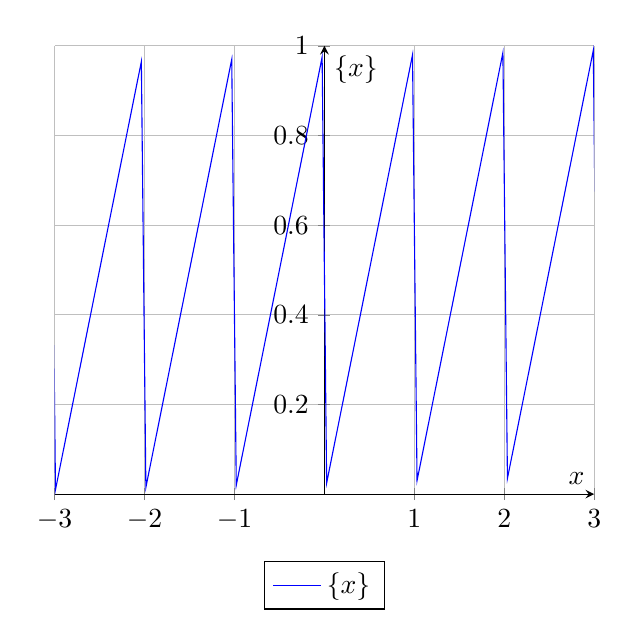
\begin{tikzpicture}
    \begin{axis}[
        xlabel={$x$},
        ylabel={$\{x\}$},
        xmin=-3, xmax=3,
        ymin=0, ymax=1,
        axis lines=middle,
        grid=both,
        legend style={at={(0.5,-0.15)},anchor=north}
    ]
    
    \addplot[blue, domain=-5:5, samples=200] {x - floor(x)};
    \legend{$\{x\}$}
    
    \end{axis}
\end{tikzpicture}

So, we can see that the minima occur at integral points. 
\end{enumerate}

\section{Curve Tracing-Root finding}

The knowledge of maxima and minima can very well be used to figure out what the graph of a function looks like. It can be used to get a rough idea to guess the roots of a solution and even analytically unsolvable implicit equations. Okay, so let us take some examples:

\begin{enumerate}
    \item Draw the graph of $f(x)=x^2/\sqrt{x+1}$

    As we can see, the function is not defined for $x\leq -1$; the domain is $[1, \infty )$. Now, 
    $$\lim_{x \to -1^{-}} f(x) = \infty$$
    $$\lim_{x to \infty} f(x) \to x^{3/2}$$

    But how does it behave in between?
    If we differentiate the function, then we get:
    $$f'(x) = \frac{x(3x+4)}{(x+1)\sqrt{x+1}}$$

    This makes it clear that the extrema is achieved at x=0; if we consider the sign of the derivative on both sides of the extrema, we figure out that this extrema is a minima. And the value of the function at this minima is 0. \textbf{The the preliminary idea is that the function decreases from $\infty$ to 0, then increases, and for large values of x, it takes the form $x^{3/2}$}

    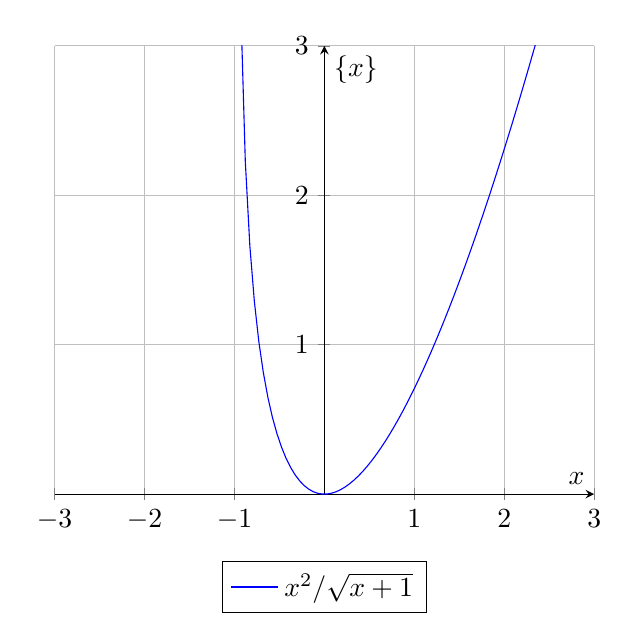
\begin{tikzpicture}
    \begin{axis}[
        xlabel={$x$},
        ylabel={$\{x\}$},
        xmin=-3, xmax=3,
        ymin=0, ymax=3,
        axis lines=middle,
        grid=both,
        legend style={at={(0.5,-0.15)},anchor=north}
    ]
    
    \addplot[blue, domain=-5:5, samples=200] {x^2/sqrt(x+1)};
    \legend{$x^2/\sqrt{x+1}$}
    
    \end{axis}
    \end{tikzpicture}

\item Let us draw the graph $xe^x$.

The domain is R. So, what happens at the extremal points?

At $x\to -\infty , f(x) \to 0$ and at $x \to \infty, f(x) \to \infty$

But what happens in between?

Let us differentiate the function and see:

$$f'(x)= (x+1)e^x$$

Thus, this function achieved a minimum at x=-1. And the value of the function, at x=-1, is -1/e.

What is happening is that the function is decreasing from 0 to -1/e and then starting to increase. At x=0, it again crosses 0 and then increases rapidly.

\begin{tikzpicture}
    \begin{axis}[
        xlabel={$x$},
        ylabel={$\{x\}$},
        xmin=-4, xmax=2,
        ymin=-1, ymax=3,
        axis lines=middle,
        grid=both,
        legend style={at={(0.5,-0.15)},anchor=north}
    ]
    
    \addplot[blue, domain=-5:5, samples=200] {x*exp(x)};
    \legend{$xe^x$}
    
    \end{axis}
    \end{tikzpicture}


\end{enumerate}

We can generalize this to more complex functions. The only thing we need to remember is that in computational sciences, where we will be calculating the differential and finding the minima, we have to remember that in real life, there are fixed algorithms for drawing near an extremum when choosing many parameters when you are optimizing. You have to be clever when choosing many parameters when you are optimizing. This means that an intuitive idea of how the function behaves is crucial. 

\textbf{By the help of maxima and minima, we can also find the nature of the roots of a cubic equation because cubic equations have pretty much known characters.}





\chapter{Differentiation in Real Life}

\section{Derivatives as Rate of Change}

Derivatives are, by definition, the rate of change of some function with respect to the independent variable. How does this rate of change come up in real-life situations?

We can only see some examples:

\begin{Enumerate}
    \item A cone with half angle $\theta$ is being filled with water at a rate $\alpha m^3/s$. The water level is already at h. Now, a nozzle at the bottom of the cone lets out water at a rate of $\beta m^3/s$, $\alpha>\beta$. Calculate the rate of change in the height of the water column.


    \begin{outline}
        Now, the net influx of water is $\alpha -\beta$, and the increase in volume in an infinitesimal time will be $dV=(\alpha-\beta)dt$; now, if the increase in height in this time period is dh. Then, the total volume increase is going to be: 
        $$dV=Adh=\pi h^2 \tan^2\theta dh$$

        Equating the two, we get:
        $$d\frac{dh}{dt}= \frac{\alpha-\beta}{\pi h^2 \tan^2\theta}$$
        giving the rate of change of height with respect to time.
         \end{outline}


    \item A rod is leaning against a wall. The length of the rod is l, and the angle it makes with the horizontal line is $\theta$; the upper part of the rod starts to fall with a velocity v. What will be the velocity of the lower edge? What is the rate of change of angle $\theta$

    We say that the vertical length of the wall from the point of contact of the rod to the bottom is given by y, and similarly, the horizontal distance from the point of contact and the corner of the wall is given by x. The length of the rod is constant. and $\frac{dy}{dt}=-v$

    Now, $$
    \begin{aligned}
    x^2+y^2=c\\
    & 2x\frac{dx}{dt}+ 2y\frac{dy}{dt}=0\\
    & 2xv_x -2yv=0\\
    & v_x  = \frac{yv}{x}=v\tan\theta\\
    \end{aligned}
     $$

     And the rate of change of angle $\theta$ is, 
     $$
     \begin{aligned}
         y=l\tan\theta\\
         \frac{dy}{dt}=l\sec^2\theta \frac{d\theta}{dt}\\
         -v=l\sec^2\theta \frac{d\theta}{dt}\\
         \frac{d\theta}{dt}=-\frac{v}{l}\cos^2\theta\\
     \end{aligned}$$
\end{Enumerate}



\part{Indefinite Integration\\ \quad in one variable}



\chapter{Introduction-motivation}

Now, we have discussed differentials in one variable in detail. Now, given there is a quantity that is a function of an independent variable, we could calculate the rate of change of the quantity concerning the change in the independent variable.

But now, we can ask ourselves, can we do the reverse? The answer is, well, yes. But only sometimes in an analytical manner. The basic knowledge of integrals starts from there. 

Integral is the reverse of differentiation in the mathematical sense. It has a helpful geometric intuition also. As the differentiation represents the slope of the graph of a function, integral represents the area under the curve of a function.

In a sense, it sums up the small changes that happened(expressed as differentials) and gives out the total change or the total effect of the changes that were made. 

\section*{History of Integral Calculus}

Integral calculus, a branch of mathematics, has a rich and fascinating history that spans thousands of years. Its development can be traced back to ancient civilizations such as the Babylonians, Egyptians, and Greeks.

\begin{enumerate}
    \item \textbf{Antiquity}: The Babylonians and Egyptians made early attempts at calculating areas and volumes. They developed basic methods for finding areas of simple shapes like squares, rectangles, and triangles. The ancient Greeks, particularly Eudoxus and Archimedes, made significant contributions to the concept of integration. Archimedes, for instance, used a method similar to what we now call the method of exhaustion to approximate the area under a curve.
    
    \item \textbf{Foundations in Antiquity and Middle Ages}: During the Middle Ages, European mathematicians such as Johannes Kepler and Bonaventura Cavalieri continued to explore methods for finding areas and volumes. However, the formalization of integral calculus as we know it today began with the work of thinkers like Isaac Barrow, Pierre de Fermat, and René Descartes.
    
    \item \textbf{17th Century}: The true birth of integral calculus is often attributed to the work of Isaac Newton and Gottfried Wilhelm Leibniz in the 17th century. Independently, both Newton and Leibniz developed what is now known as the fundamental theorem of calculus, which relates to differentiation and integration. Newton used his method of fluxions, which was based on the idea of instantaneous rates of change. At the same time, Leibniz introduced the integral symbol ($\int$) and developed a notation system that is still in use today.
    
    \item \textbf{18th Century}: The 18th century saw significant advancements in integral calculus, with mathematicians like Leonhard Euler and Joseph-Louis Lagrange making essential contributions. Euler, in particular, expanded the scope of calculus by applying it to various fields such as physics, engineering, and number theory.
    
    \item \textbf{Rigorous Foundations}: The 19th century witnessed the development of more rigorous foundations for integral calculus, mainly through the work of mathematicians like Augustin-Louis Cauchy and Karl Weierstrass. They worked on clarifying the concepts of limits and continuity, which are essential for understanding integrals.
    
    \item \textbf{Modern Developments}: In the 20th and 21st centuries, integral calculus continued to evolve, with advancements in measure theory, functional analysis, and complex analysis. Today, integral calculus is crucial in various fields, including physics, engineering, economics, and computer science.
\end{enumerate}

Throughout its history, integral calculus has undergone numerous refinements and developments. Still, its fundamental principles remain deeply rooted in ancient civilizations' work and mathematicians' pioneering efforts over the centuries.

\section{Uses}

Just like differential calculus, integral calculus is a very important part of solving real-world problems. 

\section*{Uses of Integral Calculus}

Integral calculus finds applications across various fields due to its versatility and power. Some of its common uses include:

\begin{enumerate}
    \item \textbf{Physics}: Integral calculus is extensively used in physics for solving problems related to motion, forces, energy, electricity, magnetism, and fluid dynamics. For example, calculating work done by a force, finding the center of mass of a system, determining heat transfer, and analyzing mass distribution in solid objects all involve integral calculus.
    
    \item \textbf{Engineering}: Engineers utilize integral calculus to design and analyze systems and structures. Applications include calculating areas, volumes, centroids, moments of inertia, and determining flow rates in fluid mechanics. Electrical engineers use integral calculus to analyze circuits and signals.
    
    \item \textbf{Economics and Finance}: Integral calculus plays a crucial role in economic and financial modeling, particularly in optimization problems such as maximizing profit or minimizing cost functions. It is also used in calculating areas under demand and supply curves to determine consumer and producer surplus.
    
    \item \textbf{Statistics}: Integral calculus is essential in probability theory and statistics for calculating probabilities, expected values, cumulative distribution functions, and probability density functions. It is used in statistical inference, hypothesis testing, and curve fitting.
    
    \item \textbf{Computer Science}: In computer science, integral calculus is applied in numerical analysis and algorithms for solving differential equations, optimization problems, and simulating dynamic systems. It is also used in image processing, data compression, and machine learning algorithms.
    
    \item \textbf{Medicine and Biology}: Integral calculus is used in modeling biological processes such as population growth, spread of diseases, pharmacokinetics, and enzyme kinetics. In medicine, it is applied in analyzing medical imaging data such as MRI and CT scans and in understanding physiological processes.
    
    \item \textbf{Geography and Geology}: Integral calculus is used in analyzing terrain features, calculating landform volumes, and determining erosion and sedimentation rates. It is also applied in geophysical modeling and studying the Earth's gravitational field.
    
    \item \textbf{Chemistry}: Chemists use integral calculus to analyze reaction kinetics, determine reaction rates, and calculate concentrations over time. It is also employed in spectroscopy, chromatography, and thermodynamics.
\end{enumerate}

These are just a few examples of the many applications of integral calculus. Its versatility and power make it a fundamental tool in scientific and engineering disciplines, contributing to the advancement of technology and our understanding of the natural world.


\section{Integrals as area}

Geometrically, integration can be thought of as finding the area under a curve. Consider a function \( f(x) \) defined over some interval \([a, b]\) on the x-axis. This is more appropriate for definite integrals, but indefinite integrals are just a way of getting there. 

\begin{enumerate}
    \item \textbf{Rectangular Approximation}: One intuitive approach is to approximate the area under the curve using rectangles. You can divide the interval \([a, b]\) into smaller subintervals and construct rectangles whose heights are determined by the function values at certain points within each subinterval. As you increase the number of rectangles and make their widths smaller (approaching zero), this approximation becomes more accurate.
    
    \item \textbf{Limiting Process}: To find the exact area under the curve, you need to take the limit as the width of the rectangles approaches zero. This limit process involves partitioning the interval \([a, b]\) into infinitely many subintervals and summing the areas of the rectangles corresponding to each subinterval. The width of each rectangle becomes infinitesimally small, and the sum becomes an integral.
    
    \item \textbf{Riemann Sum}: The integral of \( f(x) \) over the interval \([a, b]\) represents the limit of the Riemann sum as the width of the rectangles approaches zero. Mathematically, this can be represented as:
    
    \[ \int_{a}^{b} f(x) \, dx = \lim_{n \to \infty} \sum_{i=1}^{n} f(x_i^*) \cdot \Delta x \]
    
    where \( \Delta x \) is the width of each subinterval, \( x_i^* \) is a sample point within the \( i \)th subinterval, and \( n \) represents the number of subintervals.
    
    \item \textbf{Graphical Interpretation}: Geometrically, the integral of \( f(x) \) over \([a, b]\) represents the signed area between the curve \( y = f(x) \) and the x-axis within the interval \([a, b]\). If \( f(x) \) is above the x-axis, the area is counted positively, and if \( f(x) \) is below the x-axis, the area is counted negatively. The integral gives the net area.
    
    \item \textbf{Antiderivative}: Another geometric interpretation comes from the Fundamental Theorem of Calculus, which states that if \( F(x) \) is an antiderivative of \( f(x) \) on \([a, b]\), then:
    
    \[ \int_{a}^{b} f(x) \, dx = F(b) - F(a) \]
    
    This can be interpreted geometrically as the difference in the values of the antiderivative \( F(x) \) evaluated at the endpoints \( b \) and \( a \).
\end{enumerate}

In summary, integration geometrically represents finding the area under a curve, and it provides a powerful tool for solving problems related to accumulation, finding averages, computing volumes, and much more.



\begin{tikzpicture}[scale=4]
% Frame
\draw[gray, thick] (-0.3,-0.3) rectangle (3.3,2.3);
% Axes
\draw[->] (-0.2,0) -- (3,0) node[right] {$x$};
\draw[->] (0,-0.2) -- (0,2) node[above] {$y$};
% Curve
\draw[blue, thick, domain=0.2:2.8, smooth, variable=\x] plot ({\x}, {0.6*sin(3*\x r)+0.8});
% Area under the curve
\fill[pattern=north east lines, pattern color=gray] (0.2,0) -- plot[domain=0.2:2.8, smooth] ({\x}, {0.6*sin(3*\x r)+0.8}) -- (2.8,0) -- cycle;
% Vertical lines
\draw[dashed] (0.2,0) -- (0.2,0.6*sin(3*0.2 r)+0.8);
\draw[dashed] (2.8,0) -- (2.8,0.6*sin(3*2.8 r)+0.8);
% Labels
\draw (0.2,-0.05) node[below] {$a$};
\draw (2.8,-0.05) node[below] {$b$};
\draw (1.5,1.3) node {$y = f(x)$};
\draw (1.5,0.3) node {$A$};
% Axis ticks
\foreach \x in {0.2,0.4,...,2.8}
    \draw (\x,0.05) -- (\x,-0.05);
\foreach \y in {0.2,0.4,...,1.8}
    \draw (0.05,\y) -- (-0.05,\y);
\end{tikzpicture}

\begin{center}
    The picture of an integral represents the area under the curve. 
\end{center}




% ==========================================================
\printbibliography[title = {Aliquam}]

\end{document}
